
%version 2: \usepackage{hyperref}


%%%%%%%%%%%%%%%%%%%%%%%%%%%%%%%%%%%%%%%%%%%%%%%%%%%%%%%%%%%%%%%%%%%%%%%%
%Para las ecuaciones siempre es Ec.(n).
%Para las figuras siempre es Fig.n, incluso en el caption de la figura. Tambien las Tablas
%Para las referencias es [n]
%%%%%%%%%%%%%%%%%%%%%%%%%%%%%%%%%%%%%%%%%%%%%%%%%%%%%%%%%%%%%%%%%%%%%%%%

\documentclass[
reprint,
%notitlepage,
%superscriptaddress,
%groupedaddress,
%unsortedaddress,
%runinaddress,
%frontmatterverbose, 
%preprint,
%showpacs,preprintnumbers,
%nofootinbib,
%nobibnotes,
%bibnotes,
%11 pt,
amsmath,
amssymb,
%aps,
%pra,
prb,
%rmp,
%tightenlines %esto hizo el milagro de sacar los espacios en blancos estocásticos (?)
%prstab,
%prstper,
%floatfix,\textbf{}
]{revtex4-1} %Instalar primero para usarlo. Paquete malo.

%\documentclass[onecolumn, aps, amsmath,amssymb ]{article}
\usepackage{lipsum}  
\usepackage{graphicx}% Include figure files
\usepackage{subfig}
\usepackage{braket}
\usepackage{comment} %comment large chunks of text
\usepackage{dcolumn}% Align table columns on decimal point
\usepackage{bm}% bold math
%\usepackage{hyperref}% add hypertext capabilities
\usepackage[mathlines]{lineno}% Enable numbering of text and display math
%\linenumbers\relax % Commence numbering lines
\usepackage{mathtools} %% Para el supraíndice

\usepackage[nice]{nicefrac}

%%%%%%%El Señor Español%%%%%%%%%%%%%%%%%%%%%%%%%%%
\usepackage[utf8]{inputenc} %acento
\usepackage[
spanish, %El lenguaje.
es-tabla, %La tabla y no cuadro.
activeacute, %El acento.
es-nodecimaldot %Punto y no coma con separador de números
]{babel}
\usepackage{microtype} %para hacerlo más bonito :33 como vos (?) 
%%%%%%%%%%%%%%%%%%%%%%%%%%%%%%%%%%%%%%%%%%%%%%%%%%%
%%%%%%%%% Para que las imágenes se queden dónde las quiero (?
\usepackage{float}
%%%%%%%%%%
\usepackage{enumitem}
\usepackage{hyperref} % Para usar \url

%%%%%%%%Cambia a Fig de Figure%%%%%%%%%%
\makeatletter
\renewcommand{\fnum@figure}{Fig. \thefigure} 
\makeatother
%%%%%%%%%%%%%%%%%%%%%%%%%%%%%%%%%%%%%%%%
\raggedbottom

\usepackage{multirow}
\begin{document}

\title{Práctica 2: Introducción a Keras}
\author{Evelyn G. Coronel}

\affiliation{Redes Neuronales y Aprendizaje Profundo para Visión Artificial\\ Instituto Balseiro\\}

\date[]{\lowercase{\today}} 

\maketitle

\section*{Ejercicio 1}

    Considerando los valores de los inmuebles en Boston, se implementa un modelo simple de regresión lineal para predecir los precios, dadas las características de la propiedad. Este conjunto de datos es provisto por \verb|scikit| y las características que tienen los datos son, por ejemplo, índice de criminalidad en el barrio, edad media de los habitantes de la propiedad o los mismos son de clase baja o media para arriba.


    Previo al modelo, los datos son preprocesados restando la media y normalizando por la desviación estándar. Luego se implementa una red con una función de activación lineal, con el uso de bias y la función de costo MSE. La pérdida de la red para los datos de entrenamiento y validación se muestra en la Fig.\,\ref{fig:ejer1_loss}, utilizando `SGD' con una tasa de aprendizaje del 0.001.


    \begin{figure}[H]
        \begin{small}
            \begin{center}
                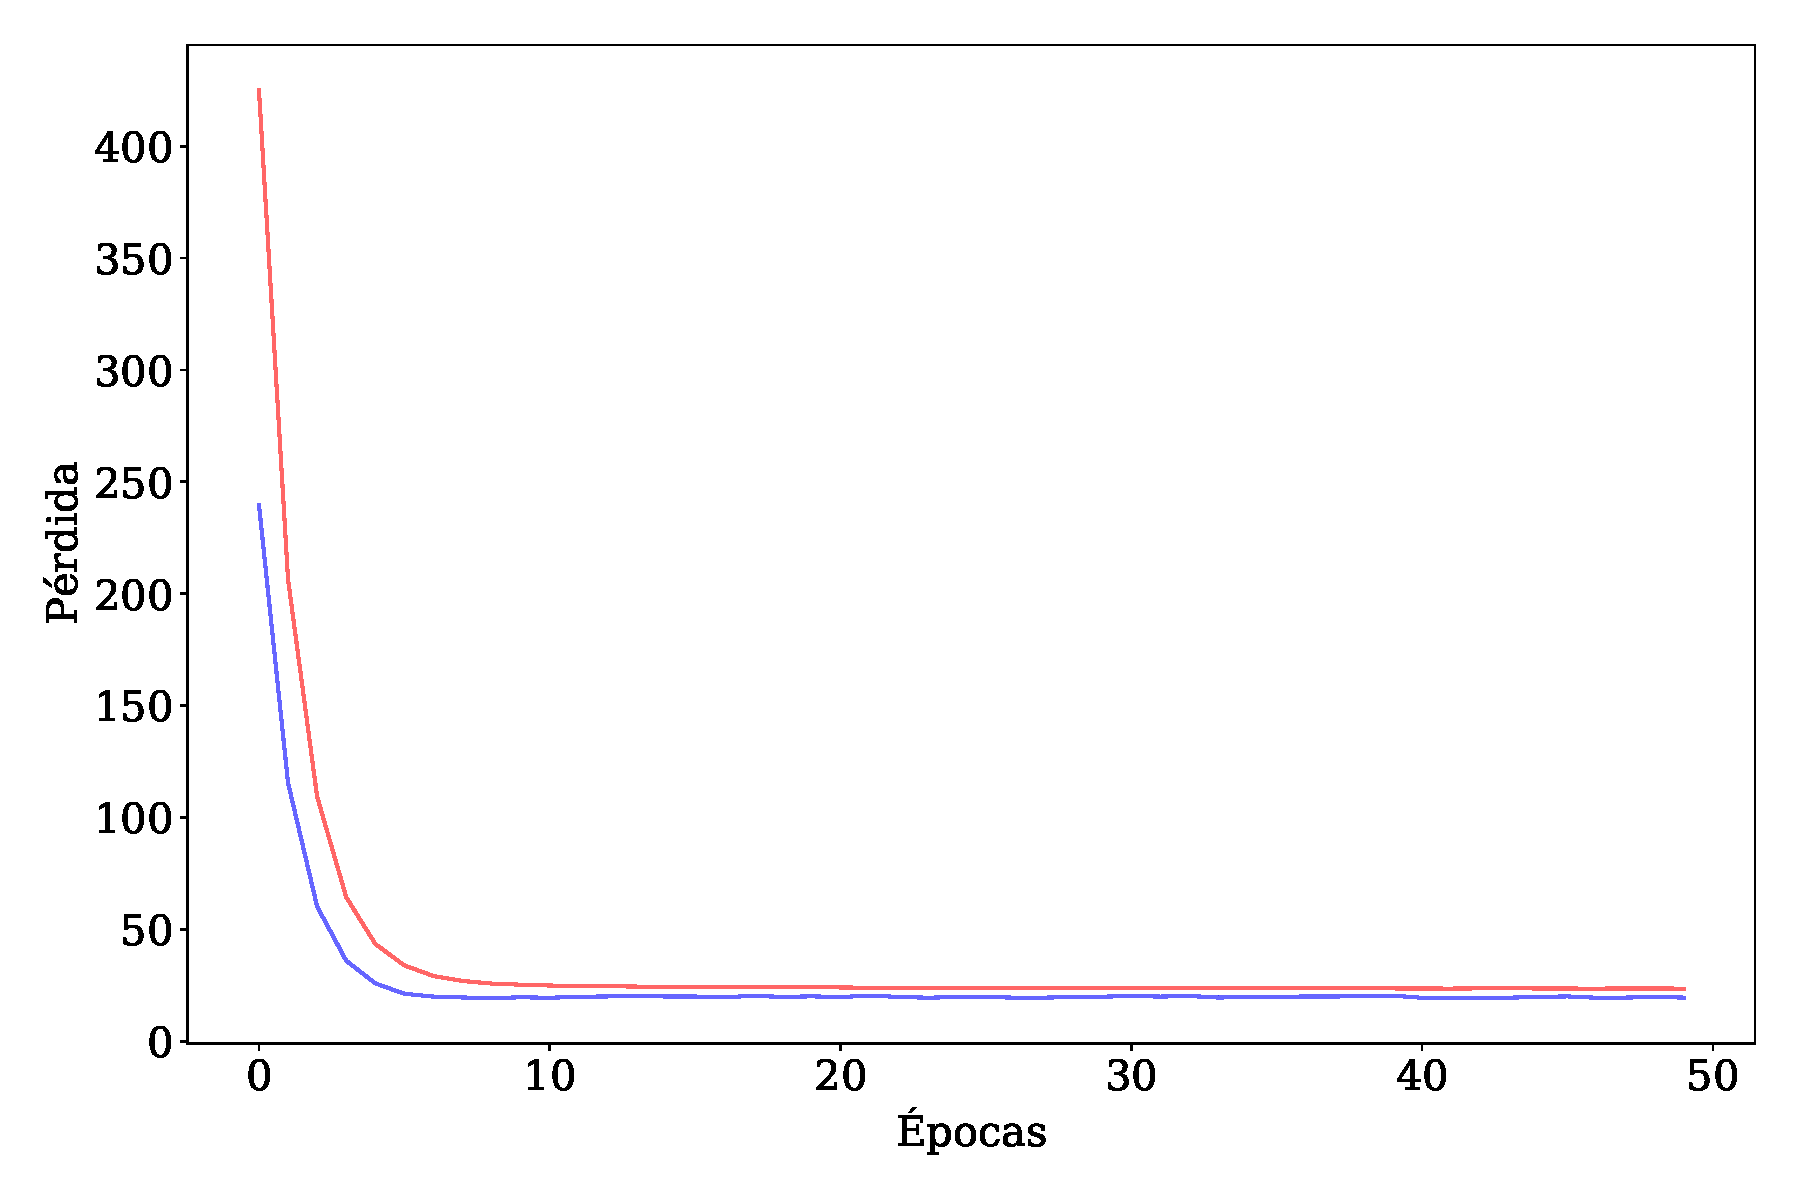
\includegraphics[width=0.5\textwidth]{Graphs/ejer1_loss.pdf}
            \end{center}
            \caption{Pérdida en función de las épocas para el ejercicio 1.}
            \label{fig:ejer1_loss}
        \end{small}
    \end{figure}

    Para dimensionar la efectividad de la red, en la Fig.\,\ref{fig:ejer1_comparacion} se muestra una comparación entre los precios reales de los inmuebles con los precios predichos por la red para los datos de validación. La línea de referencia marca los puntos donde los precios reales y predichos son iguales, se observa que la red tiene una dispersión con respecto a la referencia.

    \begin{figure}[H]
        \begin{small}
            \begin{center}
                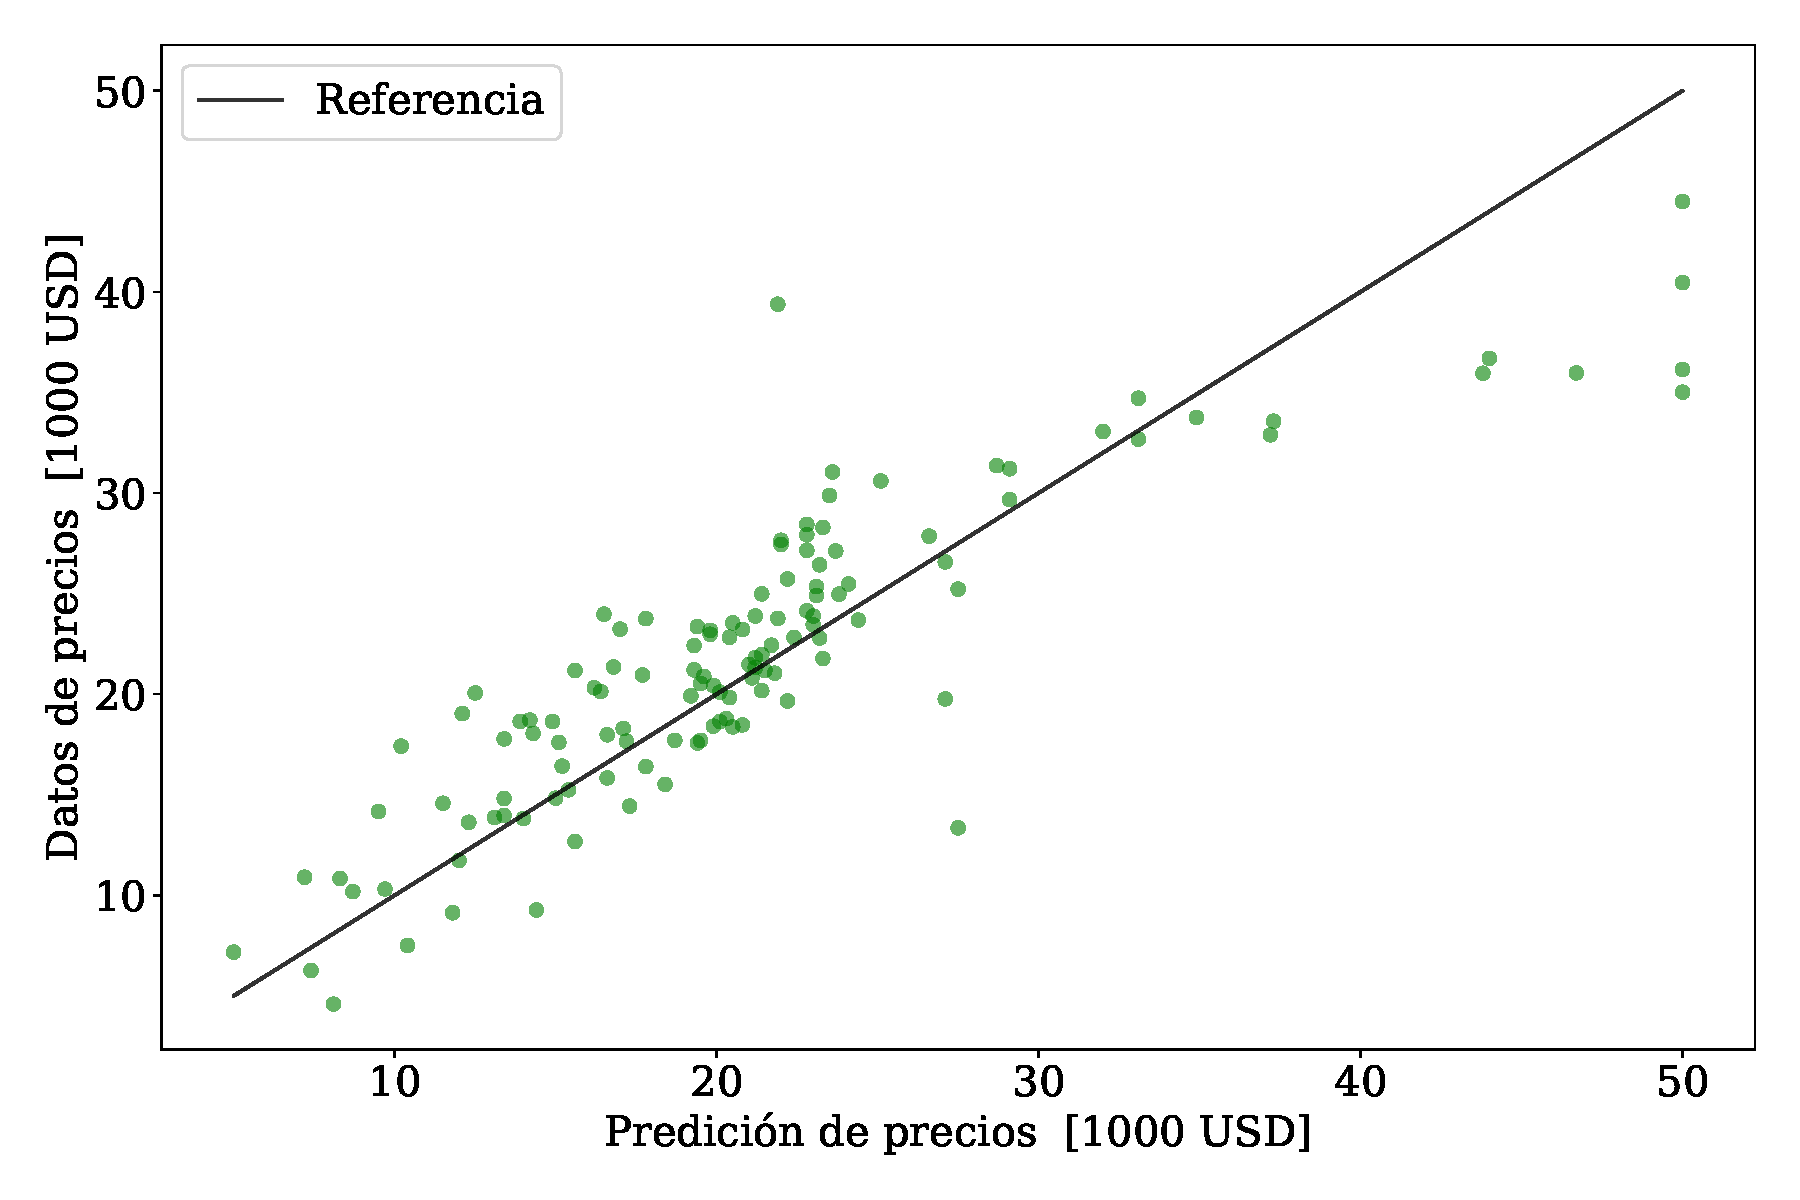
\includegraphics[width=0.5\textwidth]{Graphs/ejer1_versus.pdf}
            \end{center}
            \caption{Comparación de precios reales y predichos en los datos de validación}
            \label{fig:ejer1_comparacion}
        \end{small}
    \end{figure}

    Otra forma de dimensionar la efectividad de la red, es comprobar si la red capta la correlación entre una característica y el precio del inmueble. Por ejemplo, en el Fig.\,\ref{fig:ejer1_low_income} se muestran el precio de los inmuebles en función del porcentaje de personas en la clase baja, los datos en Boston dicen que los inmuebles en las zonas más  pobres tienden a tener un menor precio, esta correlación también se ve reflejado en los datos predichos por la red.

    \begin{figure}[H]
        \begin{small}
            \begin{center}
                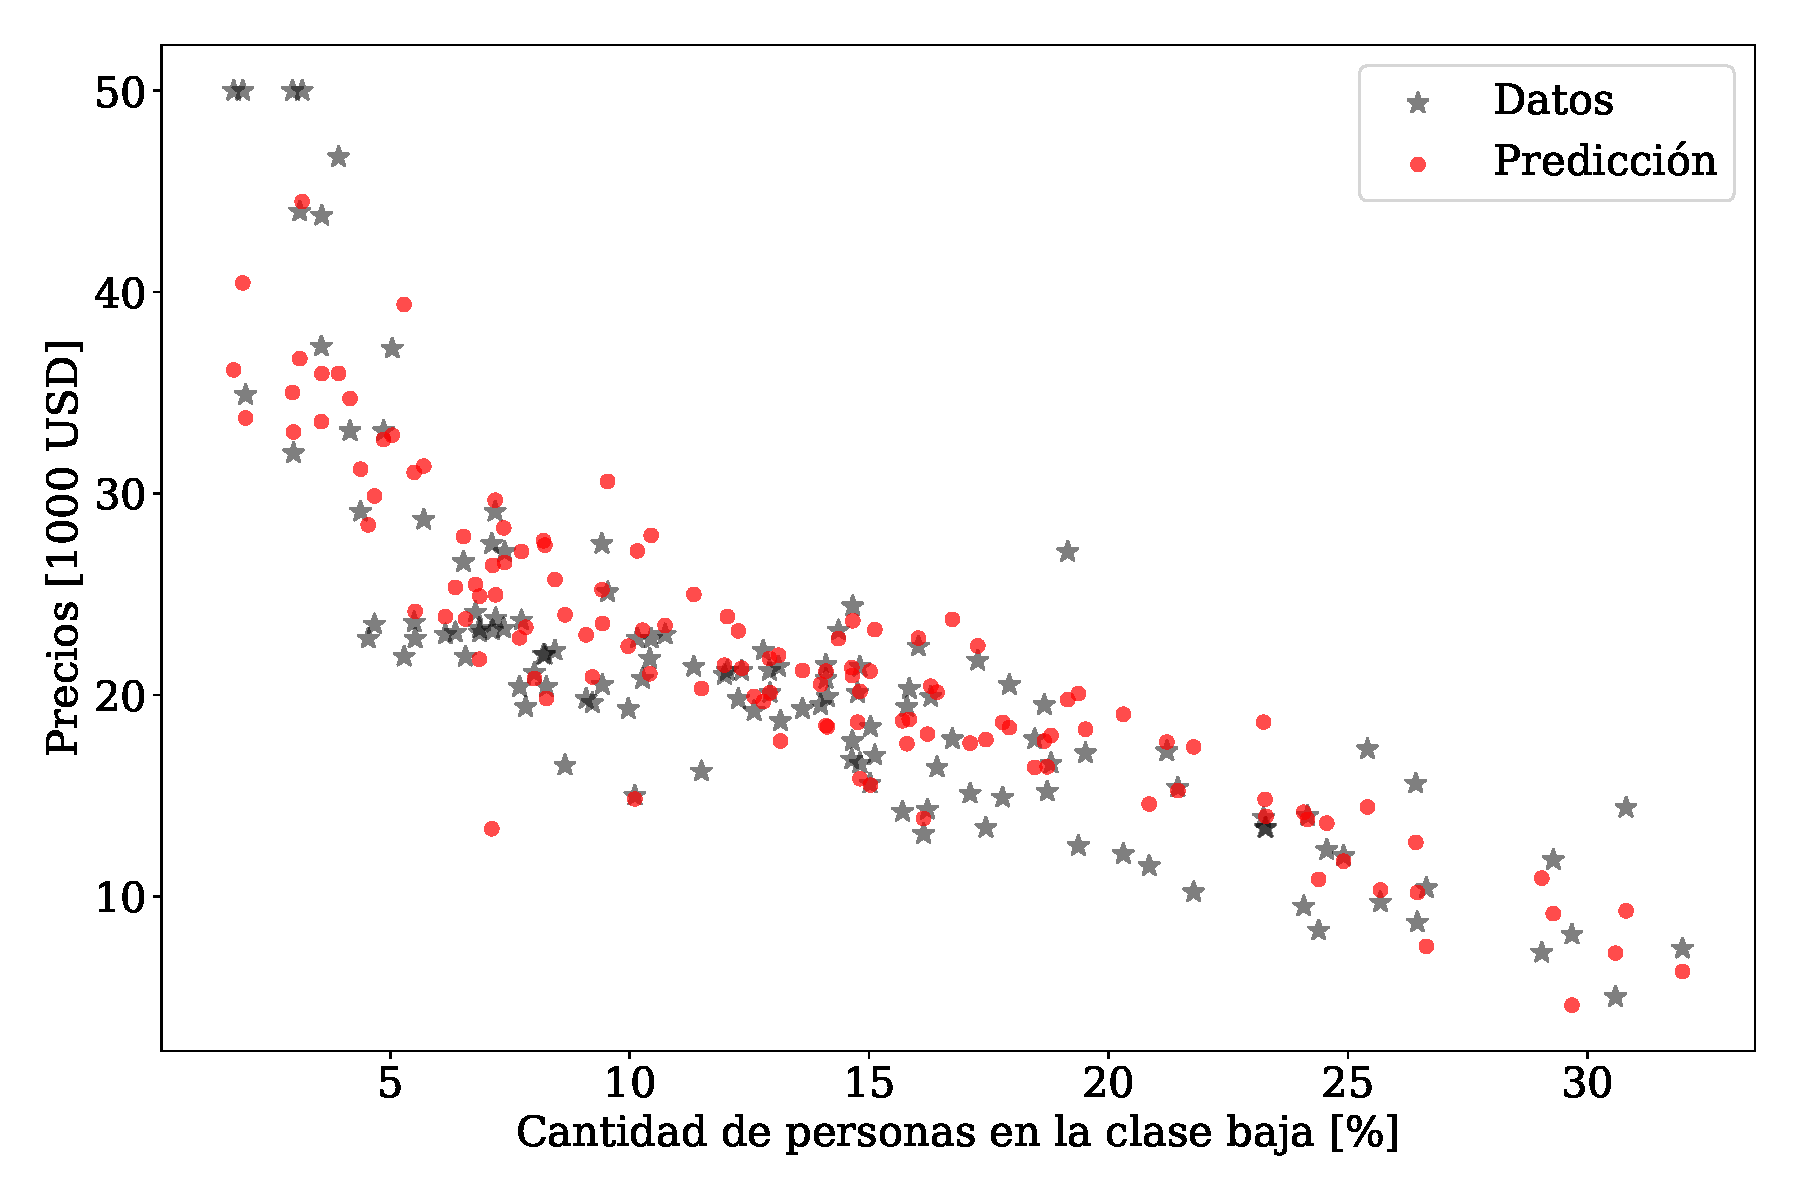
\includegraphics[width=0.5\textwidth]{Graphs/ejer1_low_income.pdf}
            \end{center}
            \caption{Precio reales y predichos de los inmuebles en función del porcentaje de personas en la clase baja}
            \label{fig:ejer1_low_income}
        \end{small}
    \end{figure}

\section*{Ejercicio 2}

\subsection*{Ejercicio 2-3}
    En este apartado se plantea clasificar el CIFAR-10 con la misma arquitectura que el problema 3 de la práctica anterior. Se usaron los mismos parámetros para comparar los resultados de \verb|Keras| con la implementación de la práctica anterior. La arquitectura es la siguiente:

    \begin{enumerate}
        \item Capa de entrada
        \item Capa Densa de 100 neuronas con bias y función de activación sigmoidal. Se utilizó el regularizador L2 con un parámetro de $10^{-4}$.
        \item Capa de salida con 10 neuronas con activación lineal y  regularizador L2 con un parámetro de $10^{-4}$.
    \end{enumerate}

    El modelo usa una función de pérdida MSE y el optimizador SGD con una tasa de aprendizaje 0.003. Las curvas de precisión y pérdida se muestran en las Figs.\ref{fig:ejer2_3_acc} y \ref{fig:ejer2_3_loss}, se observa que los resultados obtenidos con los mismos parámetros en \verb|Keras| superan a la implementación realizada en la práctica anterior.


\subsection*{Ejercicio 2-4}

    En este apartado resolvemos el ejercicio 4 de la práctica anterior con la librería \verb|Keras|, con la misma arquitectura que el apartado anterior. En uno de los puntos del ejercicio se pide usar la función de costo CCE, entonces al armar la red se utiliza la opción \verb|from_logits=True| para que internamente pase la salida por una sigmoidal para convertir los datos en probabilidades. El optimizador es SGD con una tasa de aprendizaje de 0.003 y regularizadores L2 en ambas capas con un factor de $0.0001$.

    En las Fig.\,\ref{fig:ejer2_4_acc} y \ref{fig:ejer2_4_loss} se muestran las curvas de precisión y pérdida normalizada del conjunto de validación usando la implementación propia y \verb|Keras|. Se observa que la precisión con Keras es mayor que la implementación de la práctica anterior con los mismos parámetros, aunque se tiene overfitting usando la función de costo CCE. Se probó la CCE aumentando el factor del regularizador a $0.05$ y se observa que se evita el overfitting en las primeras 500 épocas de entrenamiento.



    \subsection*{Ejercicio 2-6}

    En este apartado del ejercicio se plantea resolver nuevamente el XOR de la práctica anterior. Para estos problemas se utilizaron una tasa de aprendizaje de 0.1 y un tamaño de batch de 1, la función de pérdida utilizada fue la función MSE en ambos casos, para utilizar la métrica \verb|BinaryAccuracy| en \verb|Keras|, los datos de entrenamiento son \verb|0| y \verb|1| en cambio en la implementación propia escrita para la práctica anterior se utilizaron   \verb|-1| y \verb|1| respectivamente, además de una métrica especializada para una salida binaria entre  \verb|-1| y \verb|1|.


    \begin{figure}[H]
        \begin{small}
            \begin{center}
                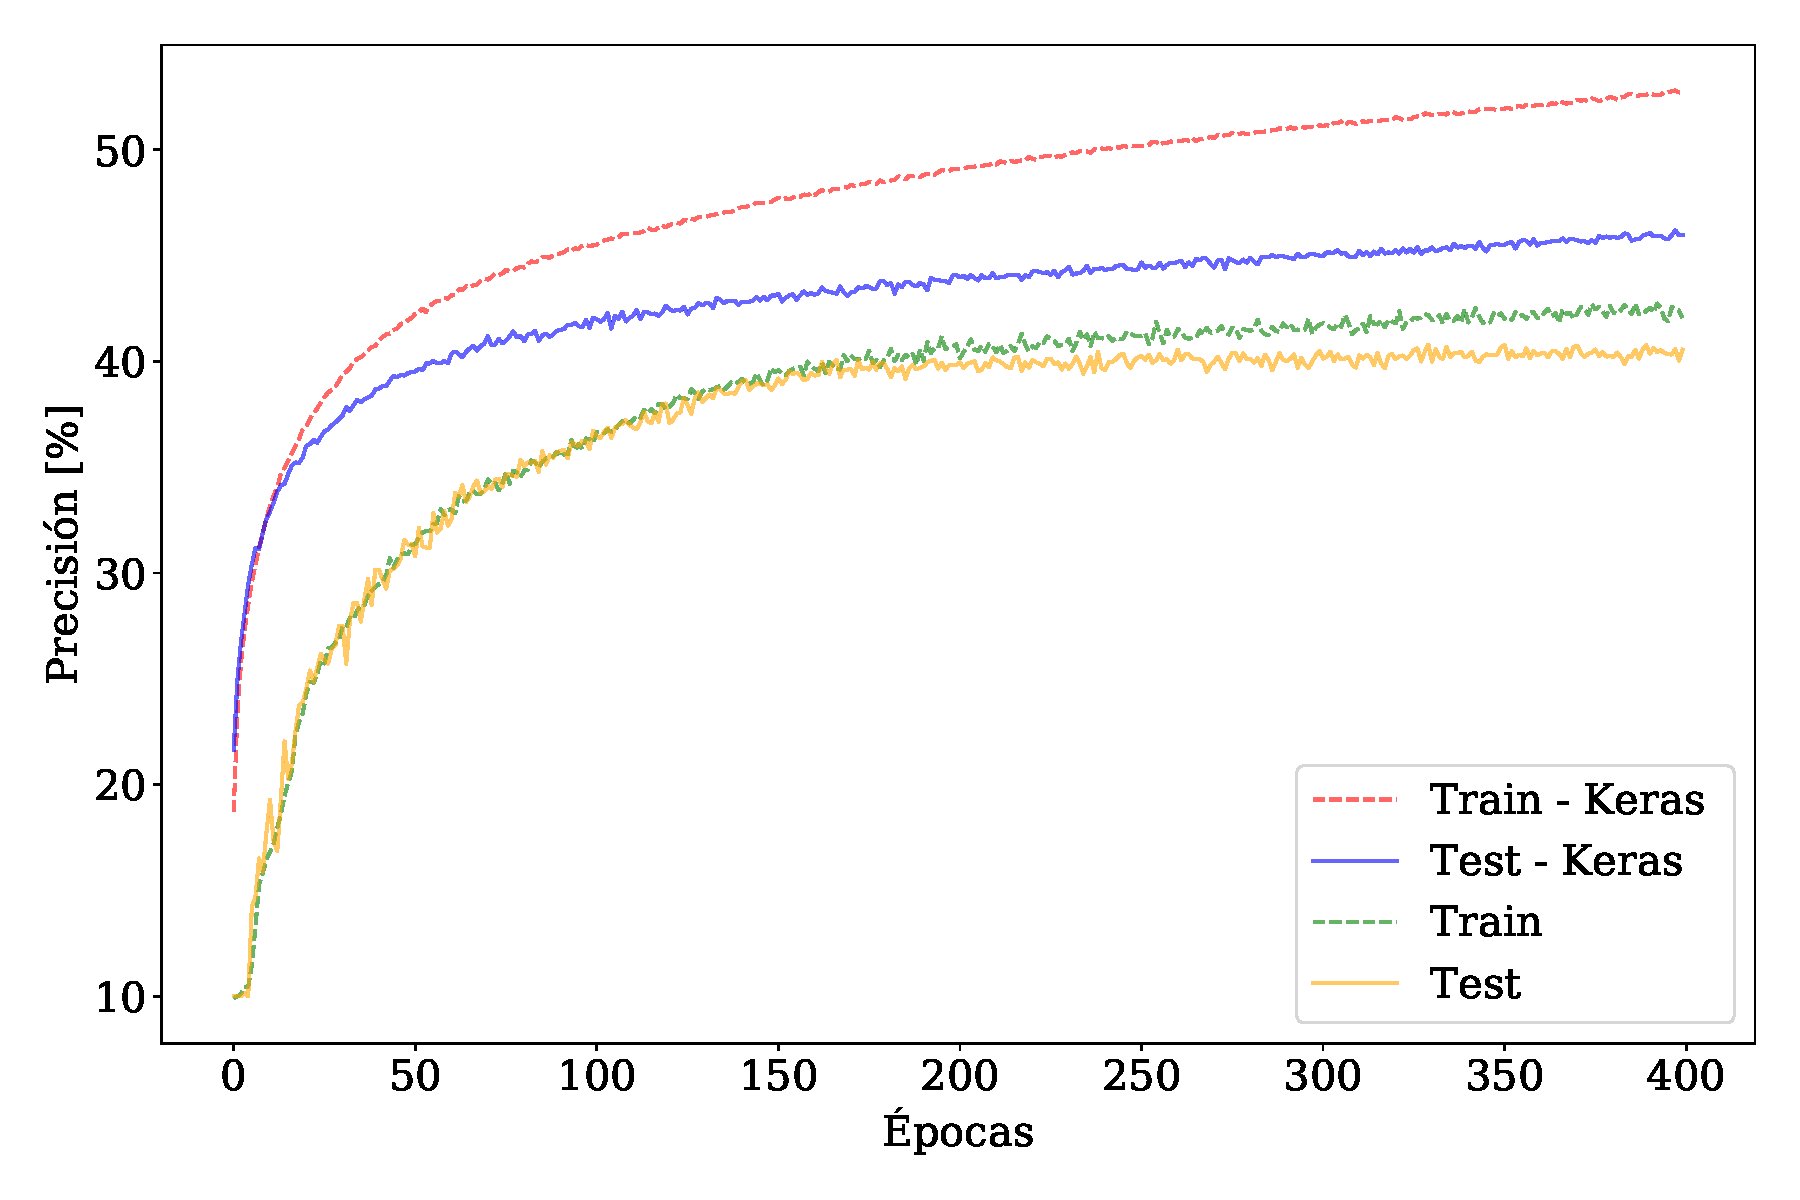
\includegraphics[width=0.5\textwidth]{Graphs/ejer2_3_acc.pdf}
            \end{center}
            \caption{Precisión de la implementación de ejercicio 3 de la práctica anterior y lo obtenido con Keras con los mismos parámetros.}
            \label{fig:ejer2_3_acc}
        \end{small}
    \end{figure}


    \begin{figure}[H]
        \begin{small}
            \begin{center}
                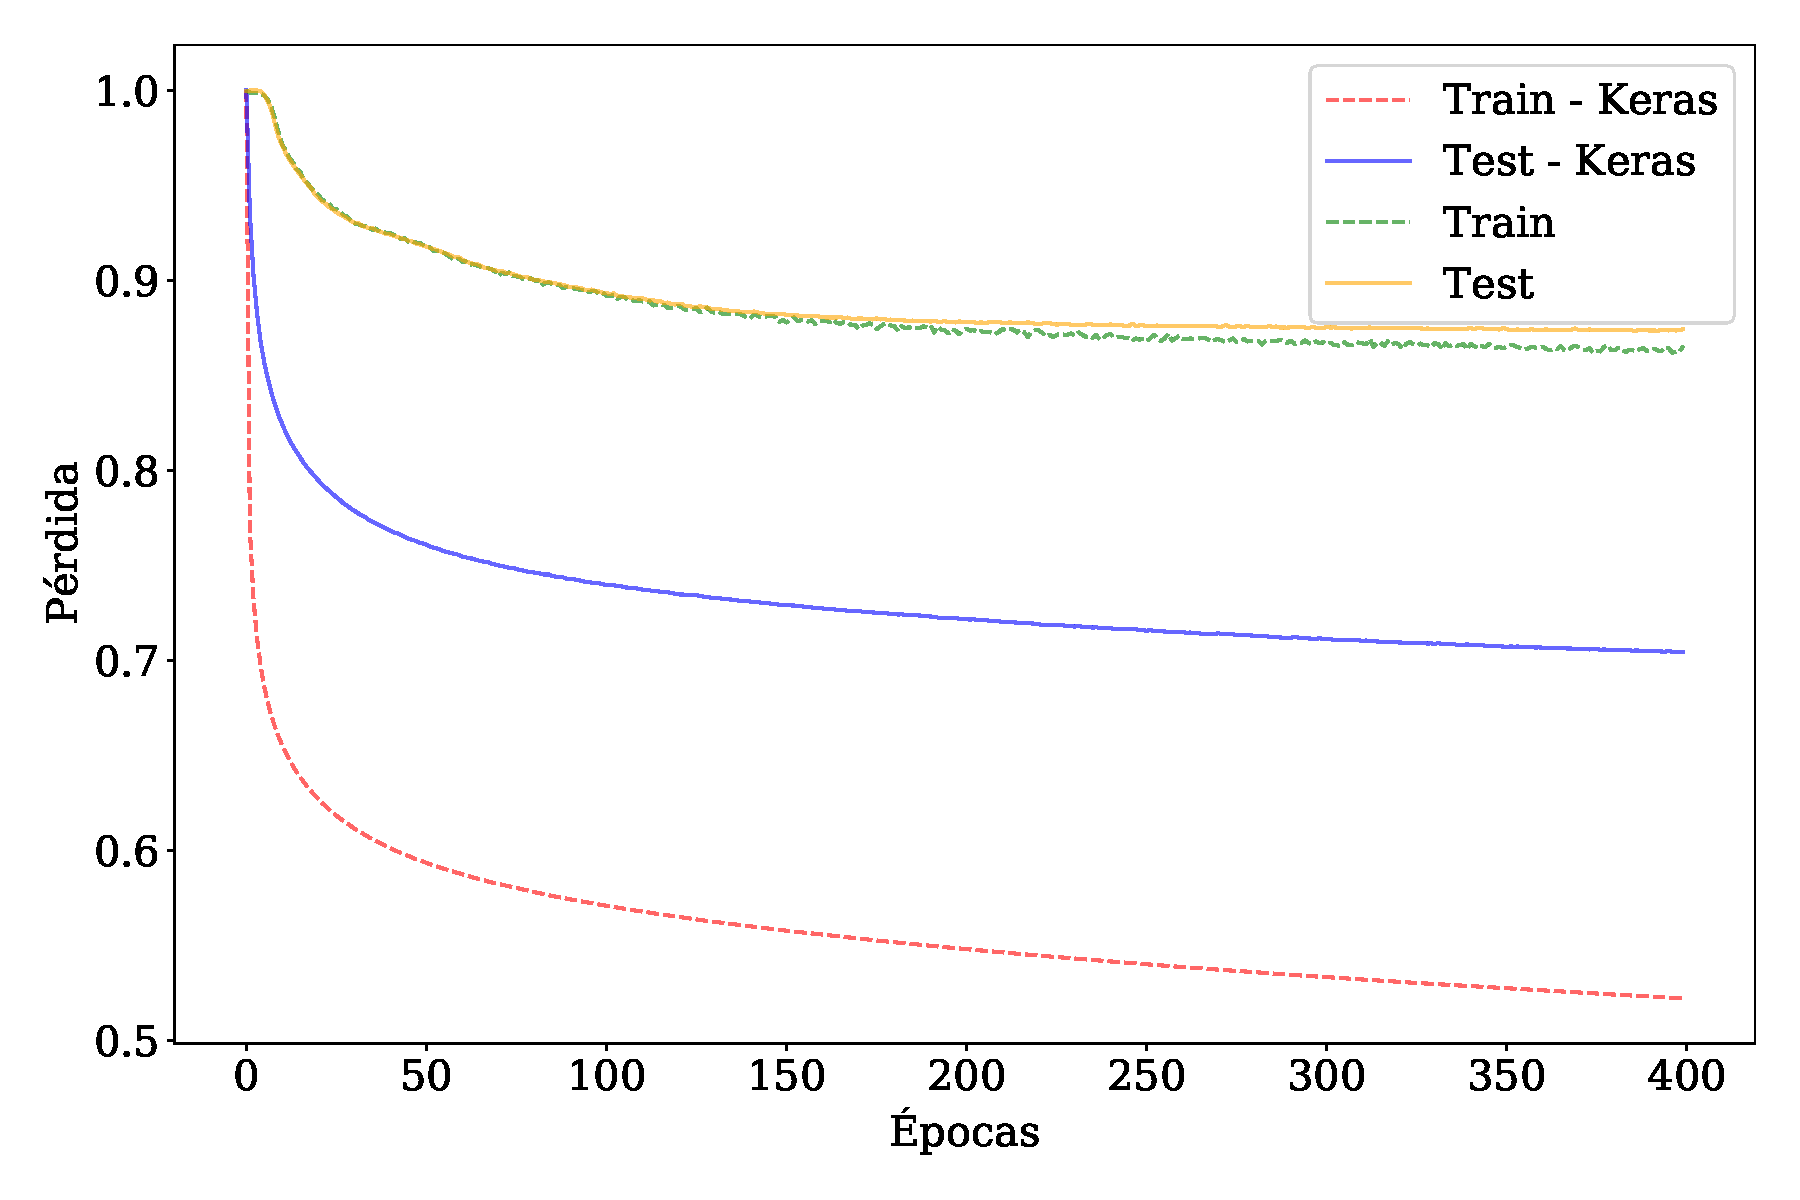
\includegraphics[width=0.5\textwidth]{Graphs/ejer2_3_loss.pdf}
            \end{center}
            \caption{Pérdida de la implementación de ejercicio 3 de la práctica anterior y lo obtenido con Keras con los mismos parámetros.}
            \label{fig:ejer2_3_loss}
        \end{small}
    \end{figure}

    %En las Fig.\ref{fig:ejer2-6-acc} y \ref{fig:ejer2-6-los} se presentan las curva de precisión y pérdida de los modelos en función de las épocas. Utilizando los módulos de \verb|Keras| se pudo observar que la arquitectura 211 en lo general tiende a converger en más épocas que la arquitectura 221.



    \section*{Ejercicio 3}

    En este ejercicio se implementa  una red densa para predecir la puntuación de una película dada la reseña. Este conjunto de datos consiste en 25000 reseñas de entrenamiento y validación, obtenidas de la página IMDB, que tiene dos posibles sentimientos: positivo o negativo, representados mediante 0 y 1.
    
    Las reseñas son listas de números que representan las palabras más usadas en inglés. El número indica cuan común es la palabra, por ejemplo la palabra representada por 1 es la palabra más común. En este ejercicio se tuvieron en cuenta las $10\,000$ palabras más usadas. El preprocesado de los datos consistió en vectorizar las reseñas de la siguiente manera: por cada reseña se tiene un vector con $10\,000$ componentes y se cuenta cuantas veces apareció un palabra en la reseña en cuestión. Por ejemplo, si la reseña contiene tres instancias de "3", la tercera componente del vector es igual a 3. Por lo tanto, tenemos un vector de $10\,000$ por cada una de las $50\,000$ reseñas.

    \begin{figure}[H]
        \begin{small}
            \begin{center}
                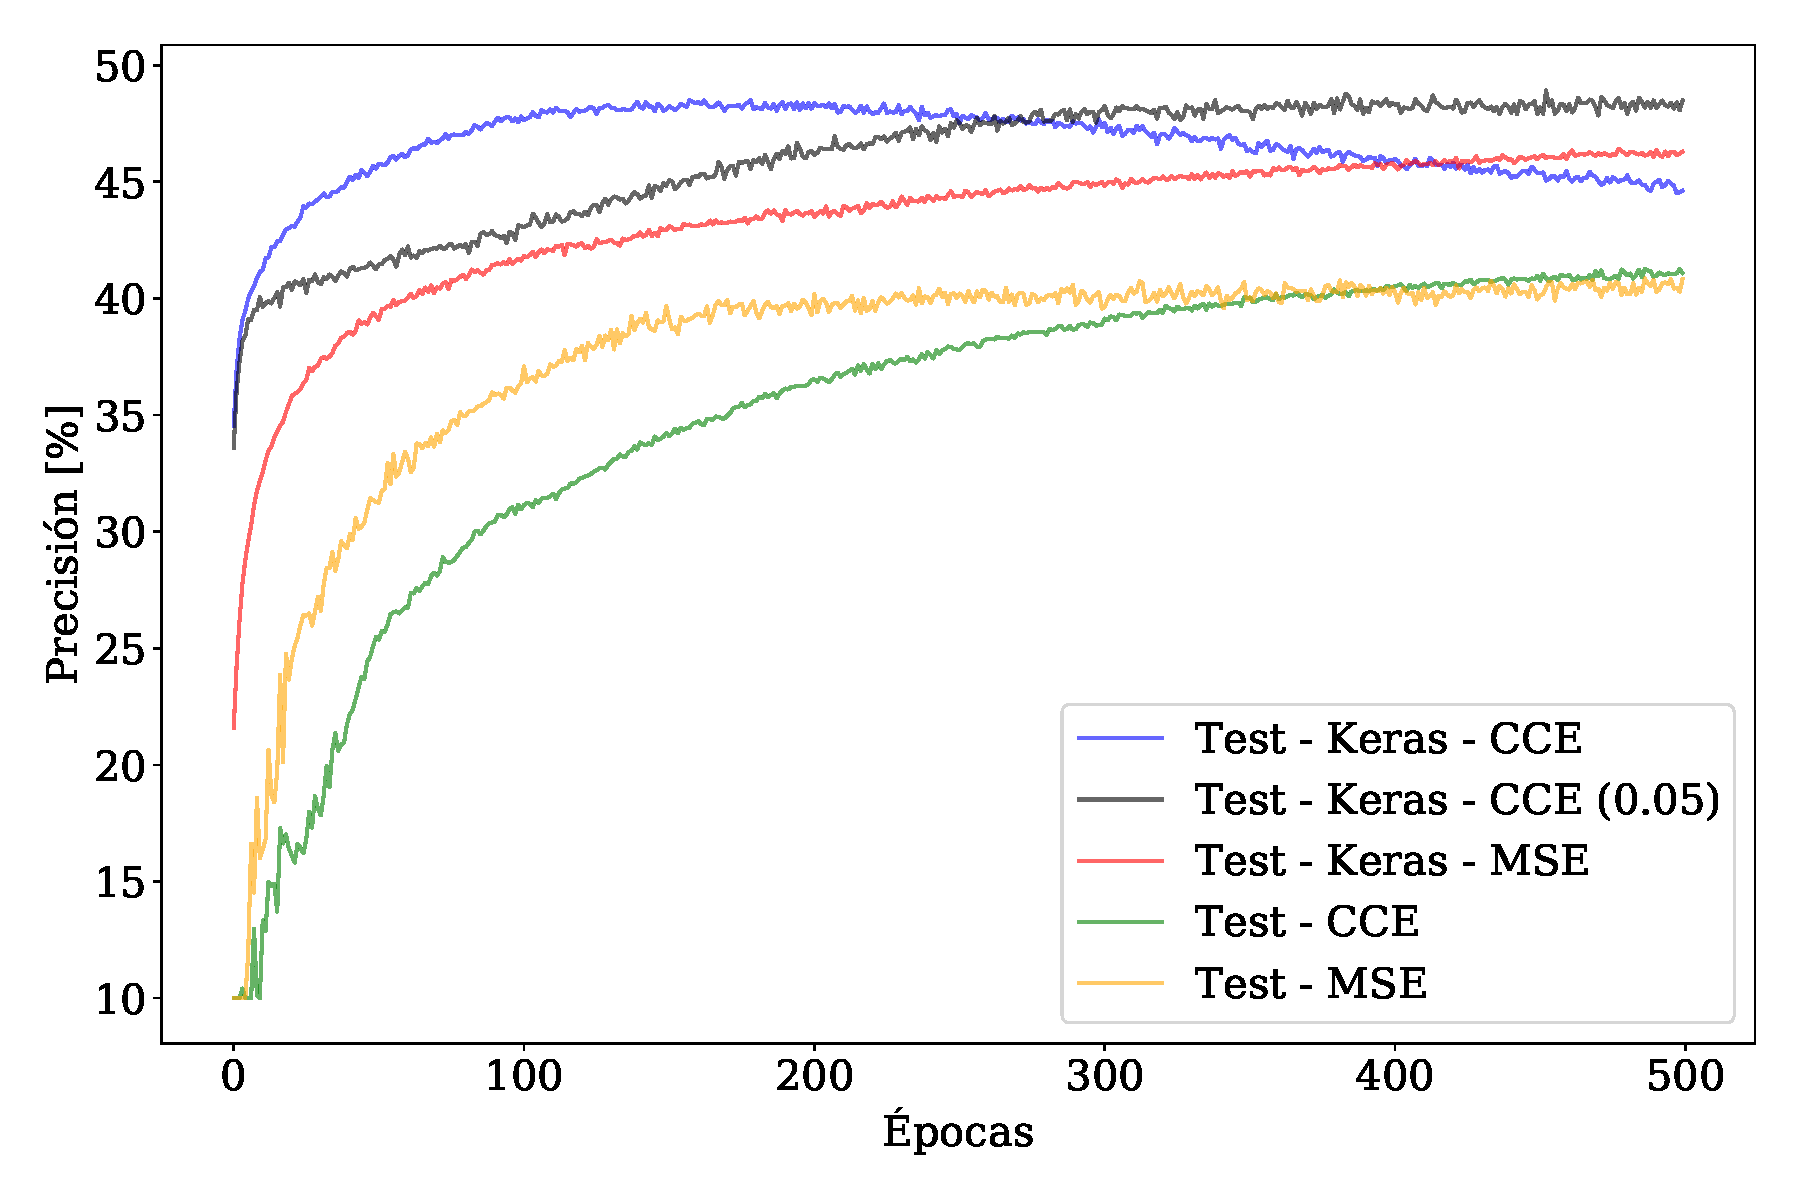
\includegraphics[width=0.5\textwidth]{Graphs/ejer2_4_acc.pdf}
            \end{center}
            \caption{Precisión de las curvas de validación para Keras y la implementación propia en el problema $2-4$. Se cambió el valor de regularización en una ejecución para mejorar la precisión.}
            \label{fig:ejer2_4_acc}
        \end{small}
    \end{figure}

    \begin{figure}[H]
        \begin{small}
            \begin{center}
                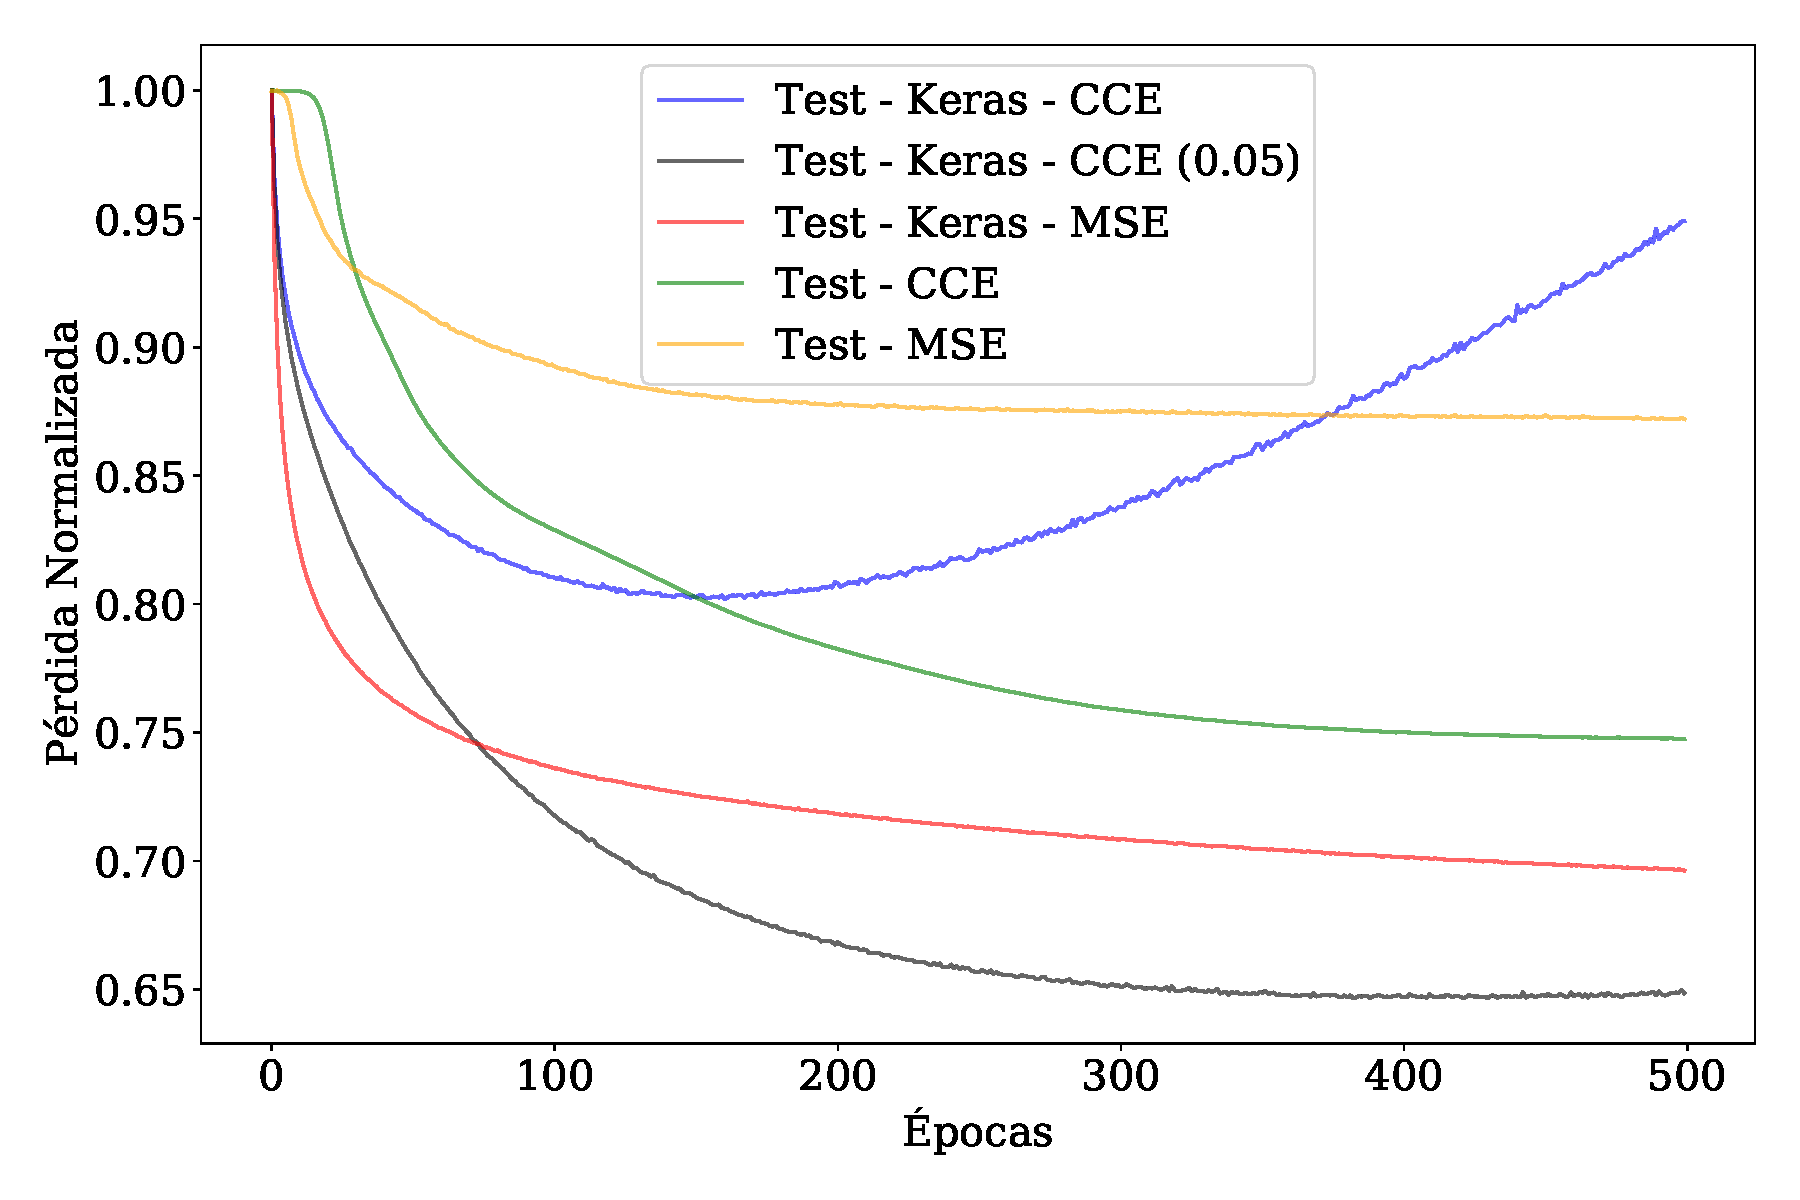
\includegraphics[width=0.5\textwidth]{Graphs/ejer2_4_loss.pdf}
            \end{center}
            \caption{Pérdida normalizada de las curvas de validación en función de las épocas en el problema $2-4$.}
            \label{fig:ejer2_4_loss}
        \end{small}
    \end{figure}

    \begin{figure}[H]
        \begin{small}
            \begin{center}
                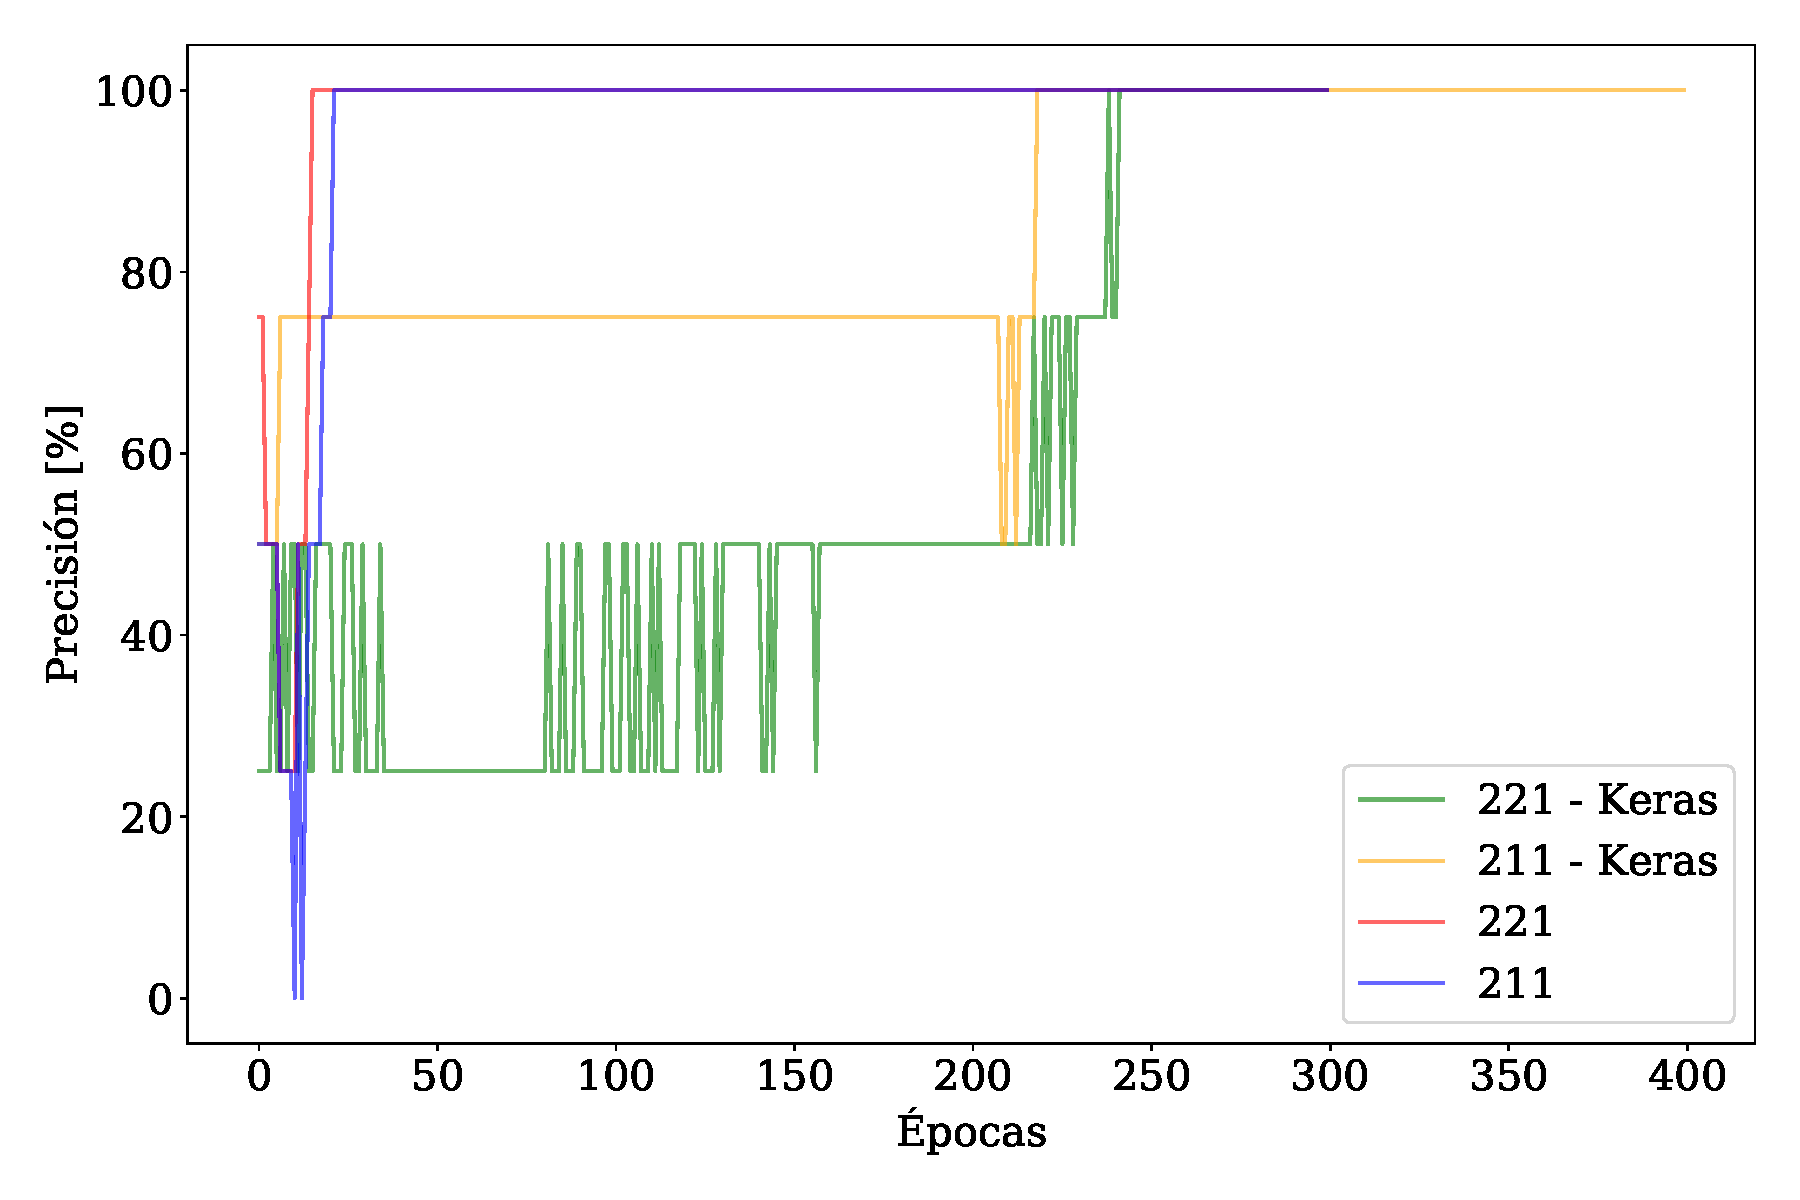
\includegraphics[width=0.5\textwidth]{Graphs/ejer2_6_acc.pdf}
            \end{center}
            \caption{Precisión en función de la épocas del problema XOR para distintas arquitectura y implementaciones de redes densas.}
            \label{fig:ejer2-6-acc}
        \end{small}
    \end{figure}

    \begin{figure}[H]
        \begin{small}
            \begin{center}
                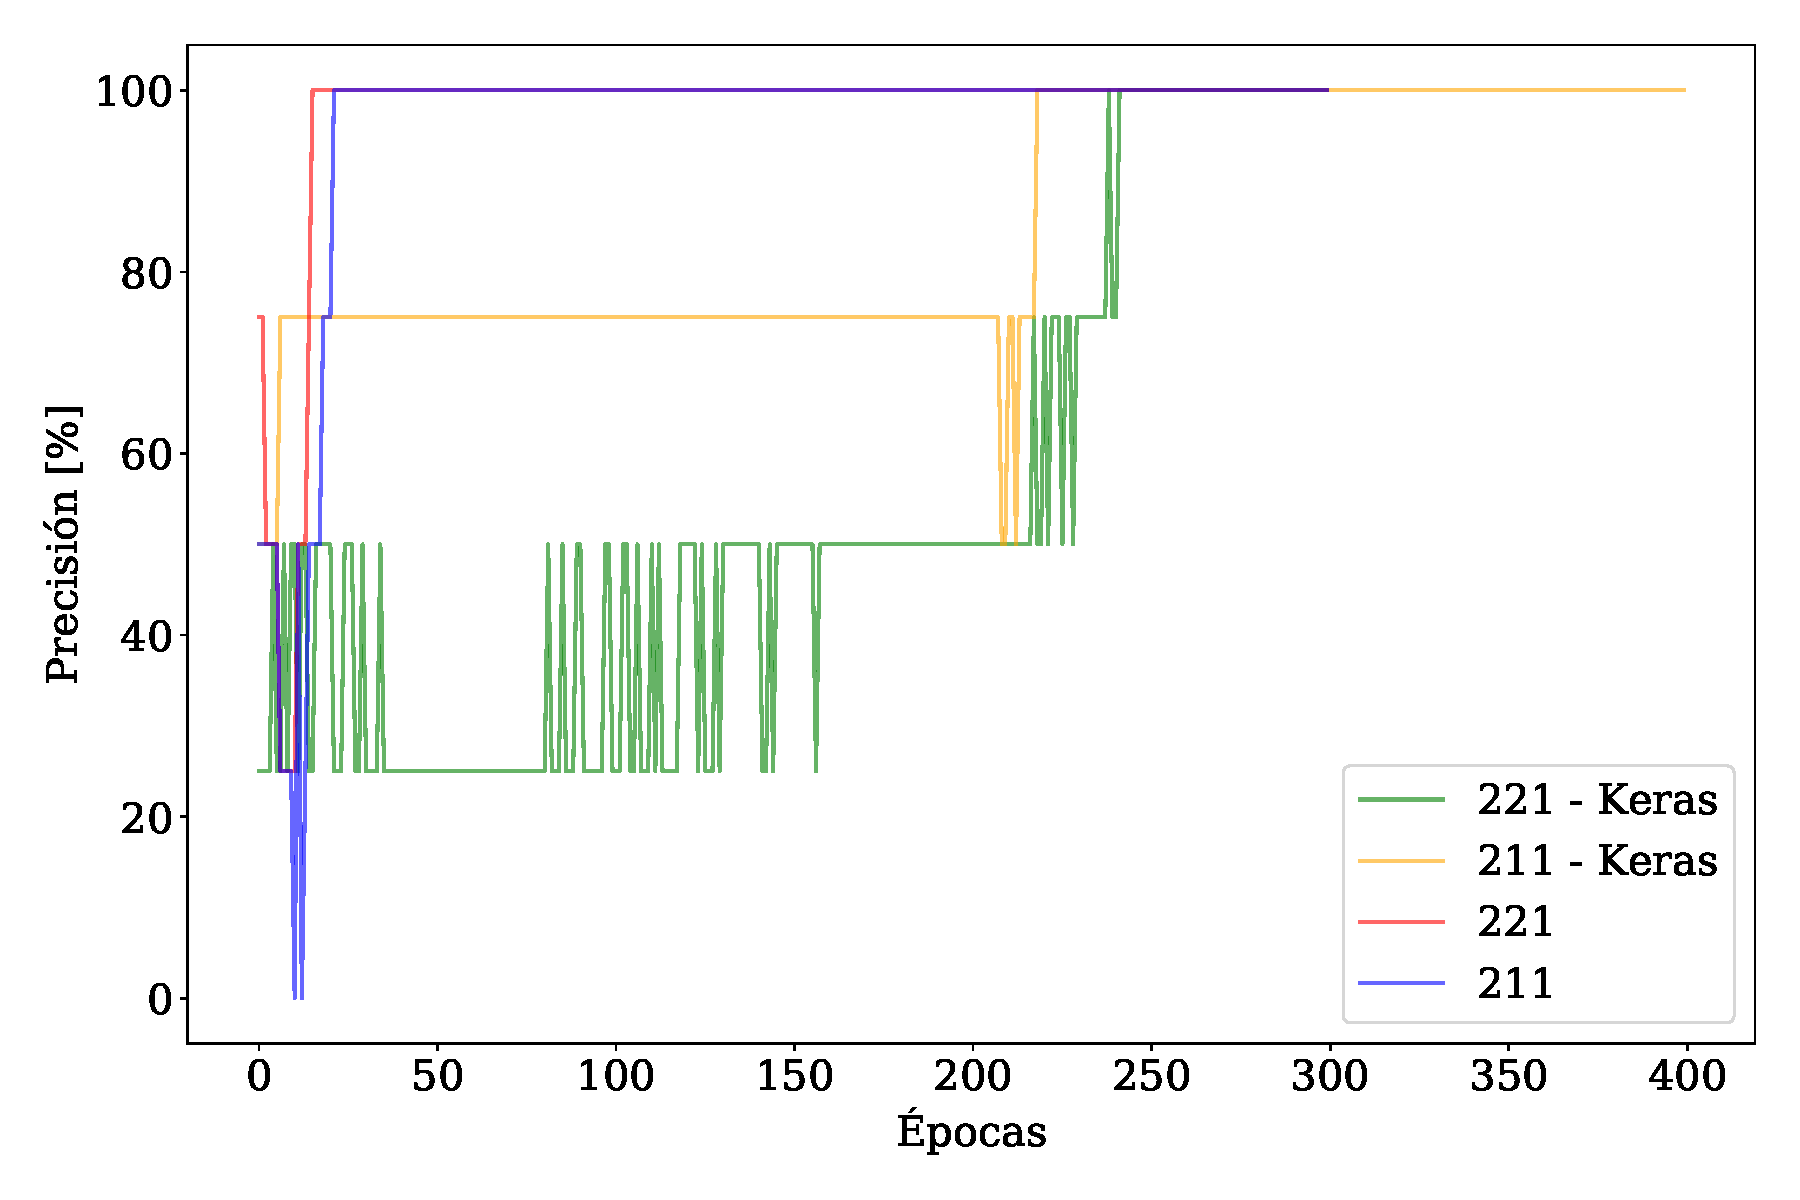
\includegraphics[width=0.5\textwidth]{Graphs/ejer2_6_acc.pdf}
            \end{center}
            \caption{Pérdida en  función de las épocas del problema XOR para distintas arquitectura y implementaciones de redes densas.}
            \label{fig:ejer2-6-los}
        \end{small}
    \end{figure}





Se implementaron distintas redes densas, donde la siguiente arquitectura arrojó la mejor precisión:

\begin{verbatim}
______________________________________________
Capa                     Salida     Parámetros 
==============================================
Densa:
Activación: ReLU          (100)     1000100   
Regularizador: L2 (0.01)
______________________________________________
Dropout (0.5)             (100)     0         
______________________________________________
Batch Normalization       (100)     400       
______________________________________________
Densa:
Activación: ReLU          (30)      3030 
Regularizador: L2 (0.01)
_______________________________________________
Dropout (0.5)             (30)      0         
_______________________________________________
Densa:
Activación: Sigmoide      (1)       31        
Regularizador: L2 (0.01) 
===============================================
Total parámetros: 1,003,561
Parámetros fijos: 200
\end{verbatim}
Esta red utiliza el optimizador SGD con una tasa de aprendizaje de $0.001$, una función de pérdida CCE y métrica \verb|BinaryAccuracy|. Los resultados de la precisión se presentan en la Fig.\ref{fig:ejer3_acc} y la evolución de la pérdida normalizada se puede ver en la Fig.\ref{fig:ejer3_loss}. La red final alcanza una precisión del $84,8\%$

\begin{figure}[H]
    \begin{small}
        \begin{center}
            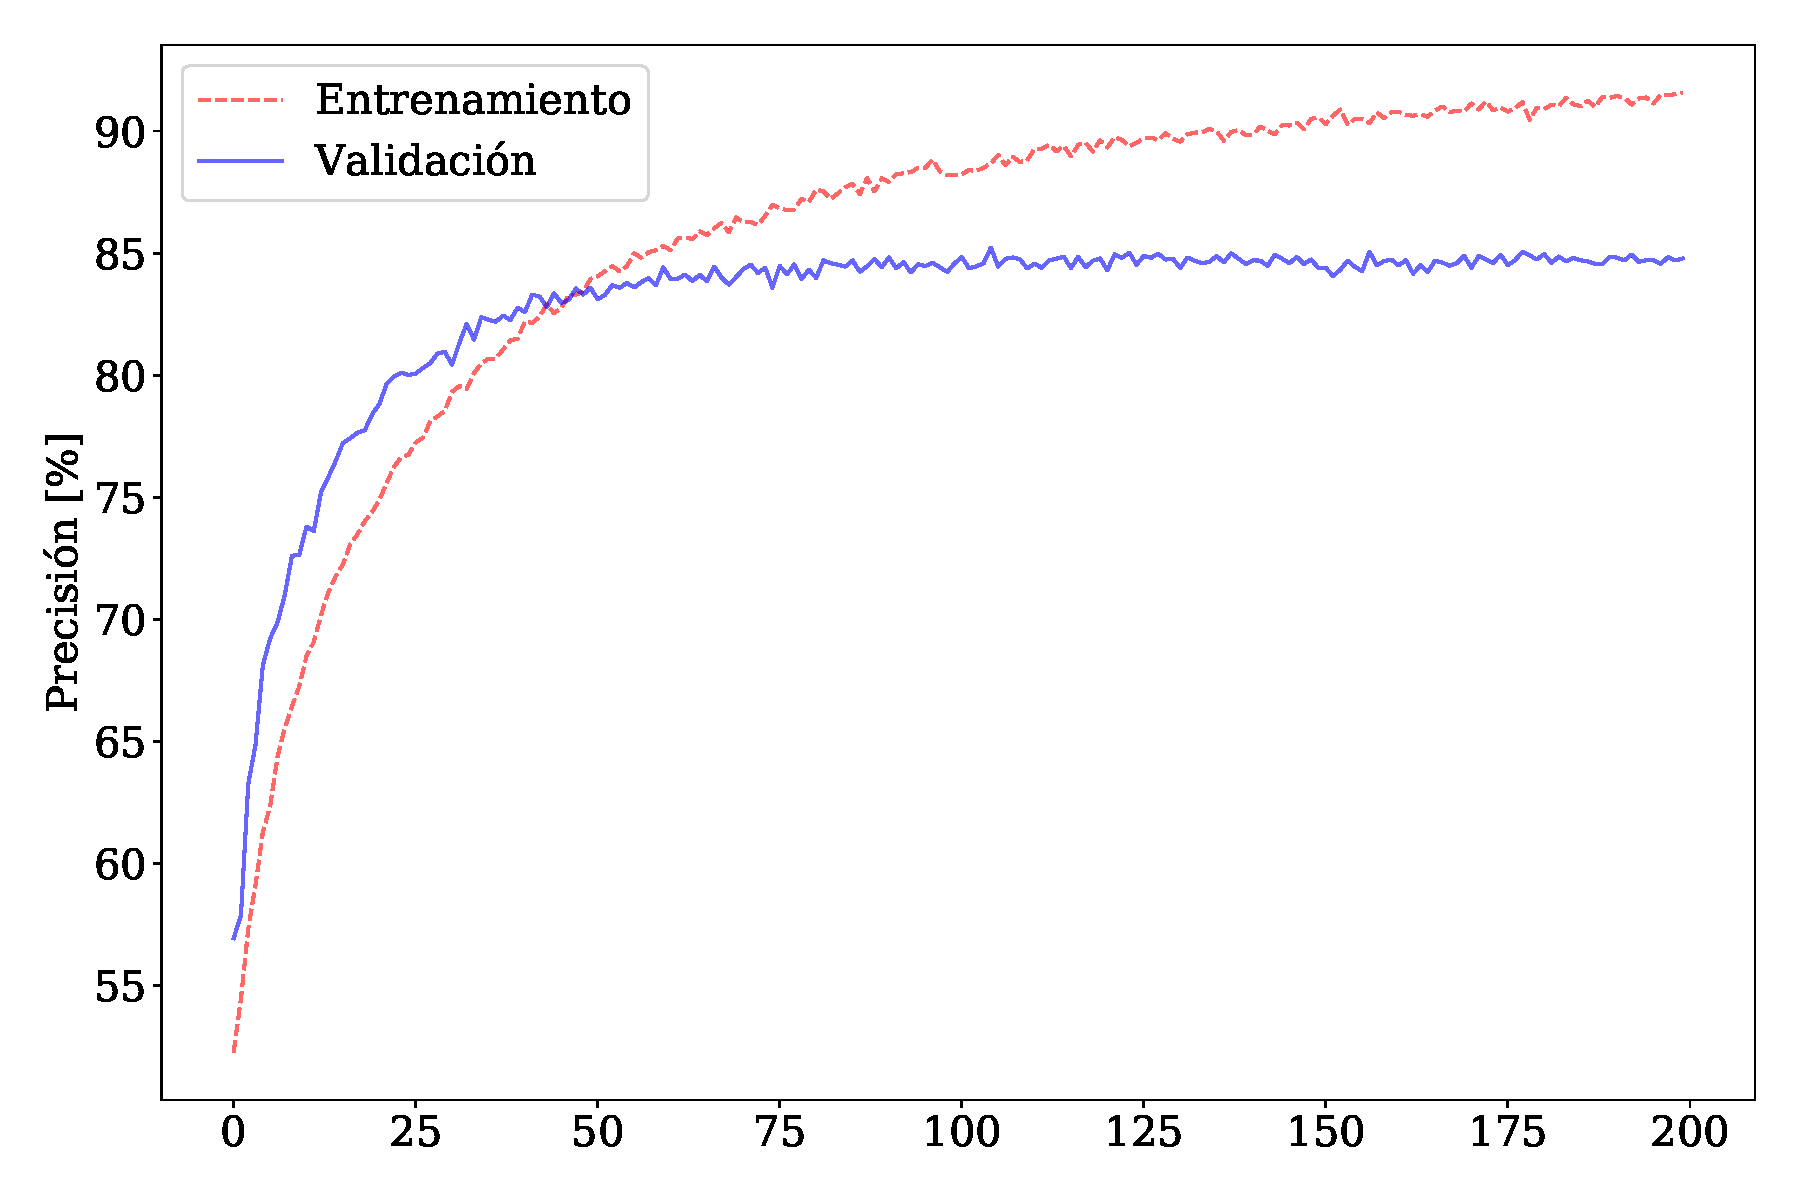
\includegraphics[width=0.5\textwidth]{Graphs/ejer3_acc.pdf}
        \end{center}
        \caption{Precisión de la red en función de las épocas}
        \label{fig:ejer3_acc}
    \end{small}
\end{figure}


\begin{figure}[H]
    \begin{small}
        \begin{center}
            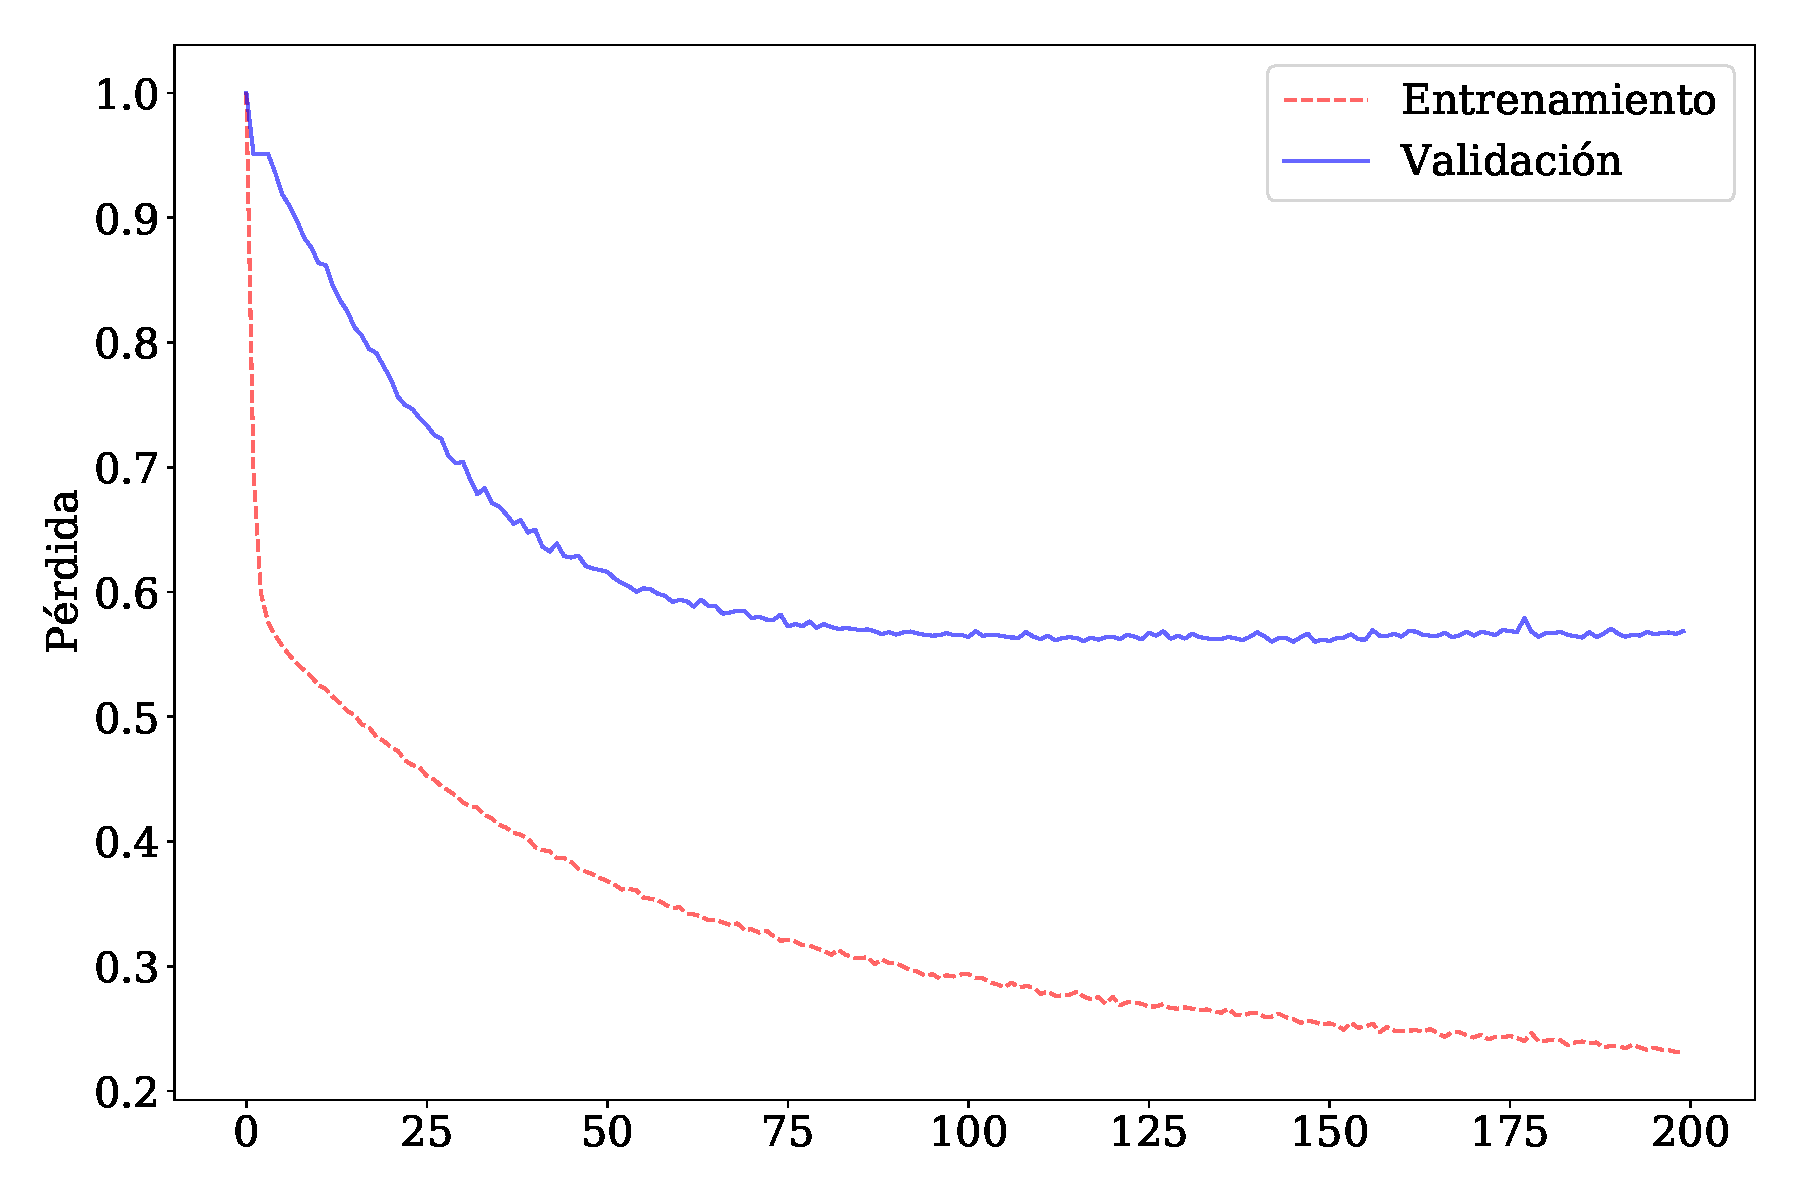
\includegraphics[width=0.5\textwidth]{Graphs/ejer3_loss.pdf}
        \end{center}
        \caption{Pérdida normalizada con respecto al máximo en función de las épocas. }
        \label{fig:ejer3_loss}
    \end{small}
\end{figure}

Dado que la red tiene varios tipos de capas que fueron agregándose para mejorar la precisión y evitar el overfitting, en las Figs.\ref{fig:ejer3_acc_trails} y \ref{fig:ejer3_los_trails} se muestran la precisión y pérdida para los datos de validación para redes sin ciertas capas. La curva denominada como \emph{Simple} es la red densa sin ninguna capa especial. La precisión de la curva de la red final y sin Dropouts parecieran llegar a una precisión similar, pero si se observa la pérdida, la red sin Dropout presenta overfitting.

\begin{figure}[H]
    \begin{small}
        \begin{center}
            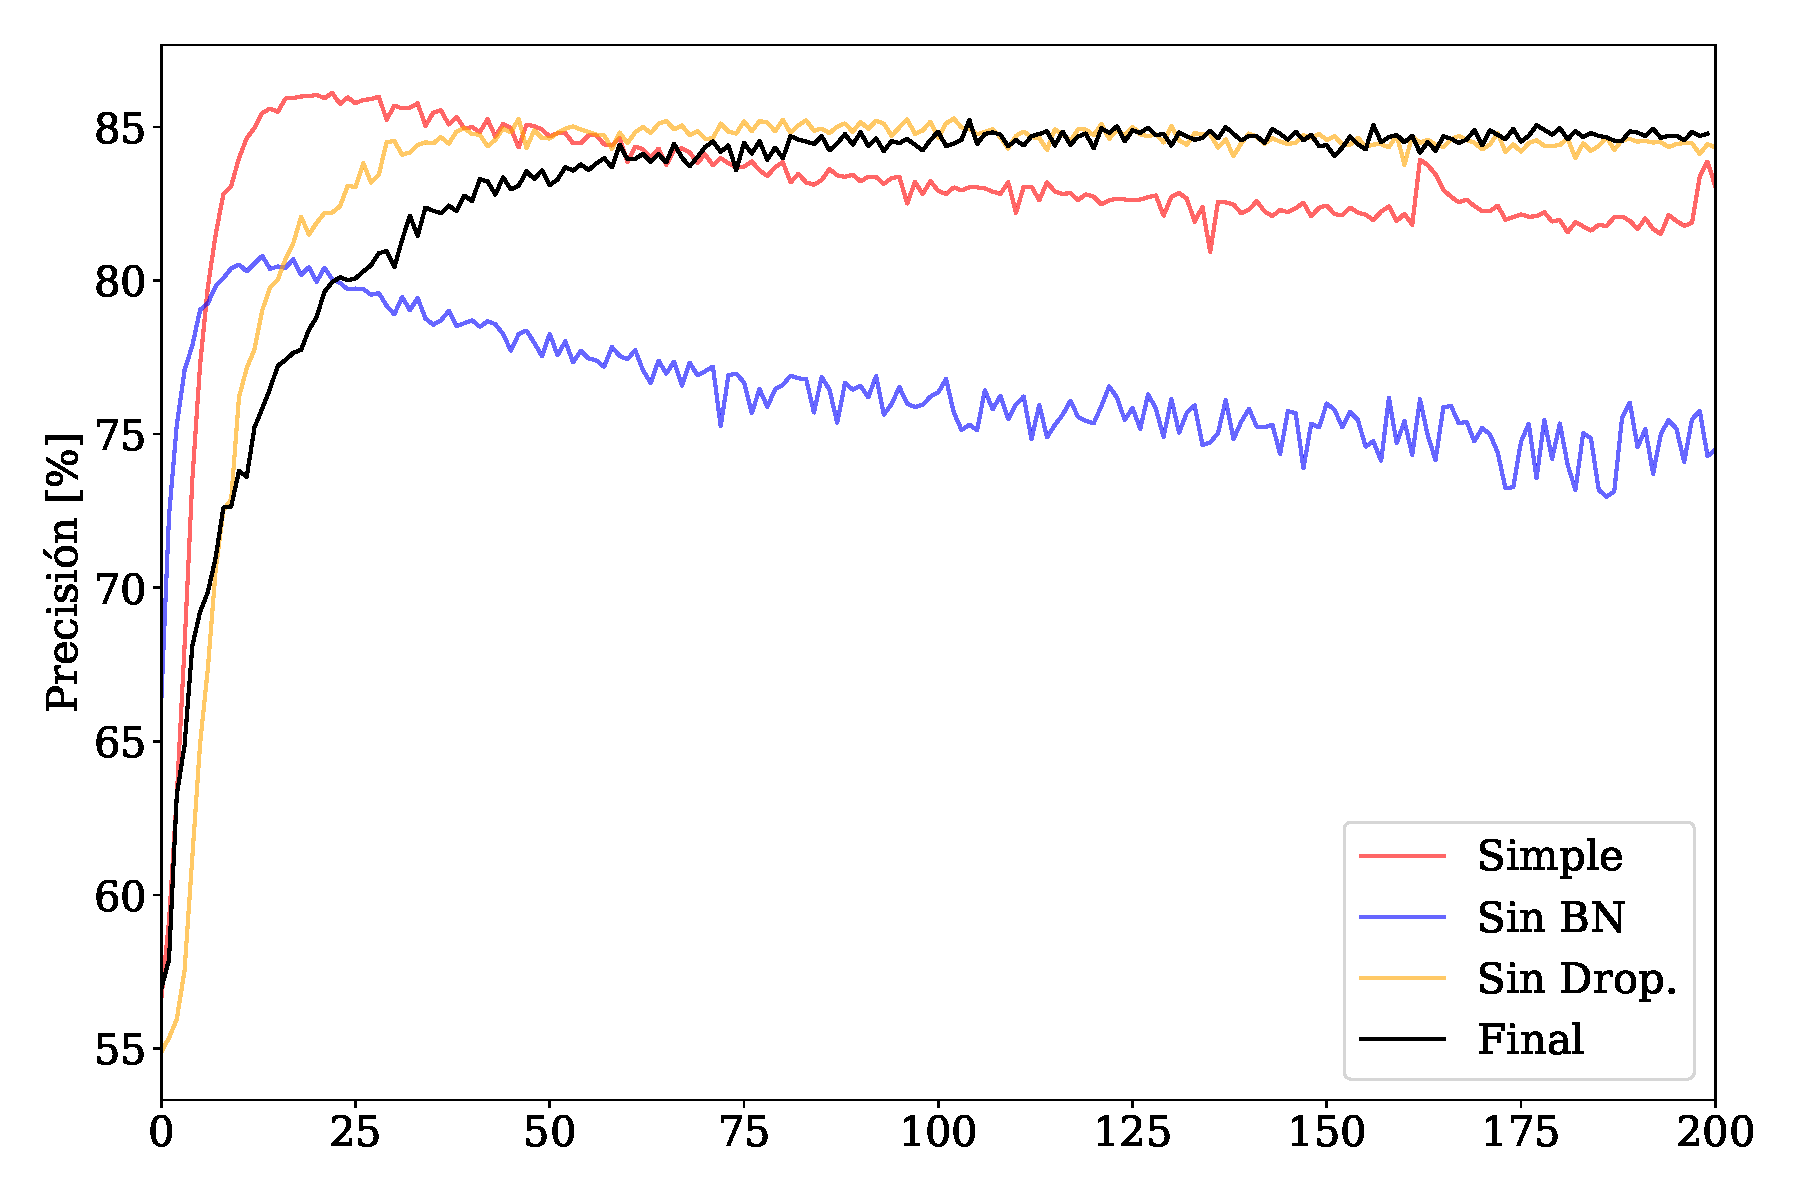
\includegraphics[width=0.5\textwidth]{Graphs/ejer3_acc_trails.pdf}
        \end{center}
        \caption{Precisión de las redes en función de las épocas. }
        \label{fig:ejer3_acc_trails}
    \end{small}
\end{figure}


\begin{figure}[H]
    \begin{small}
        \begin{center}
            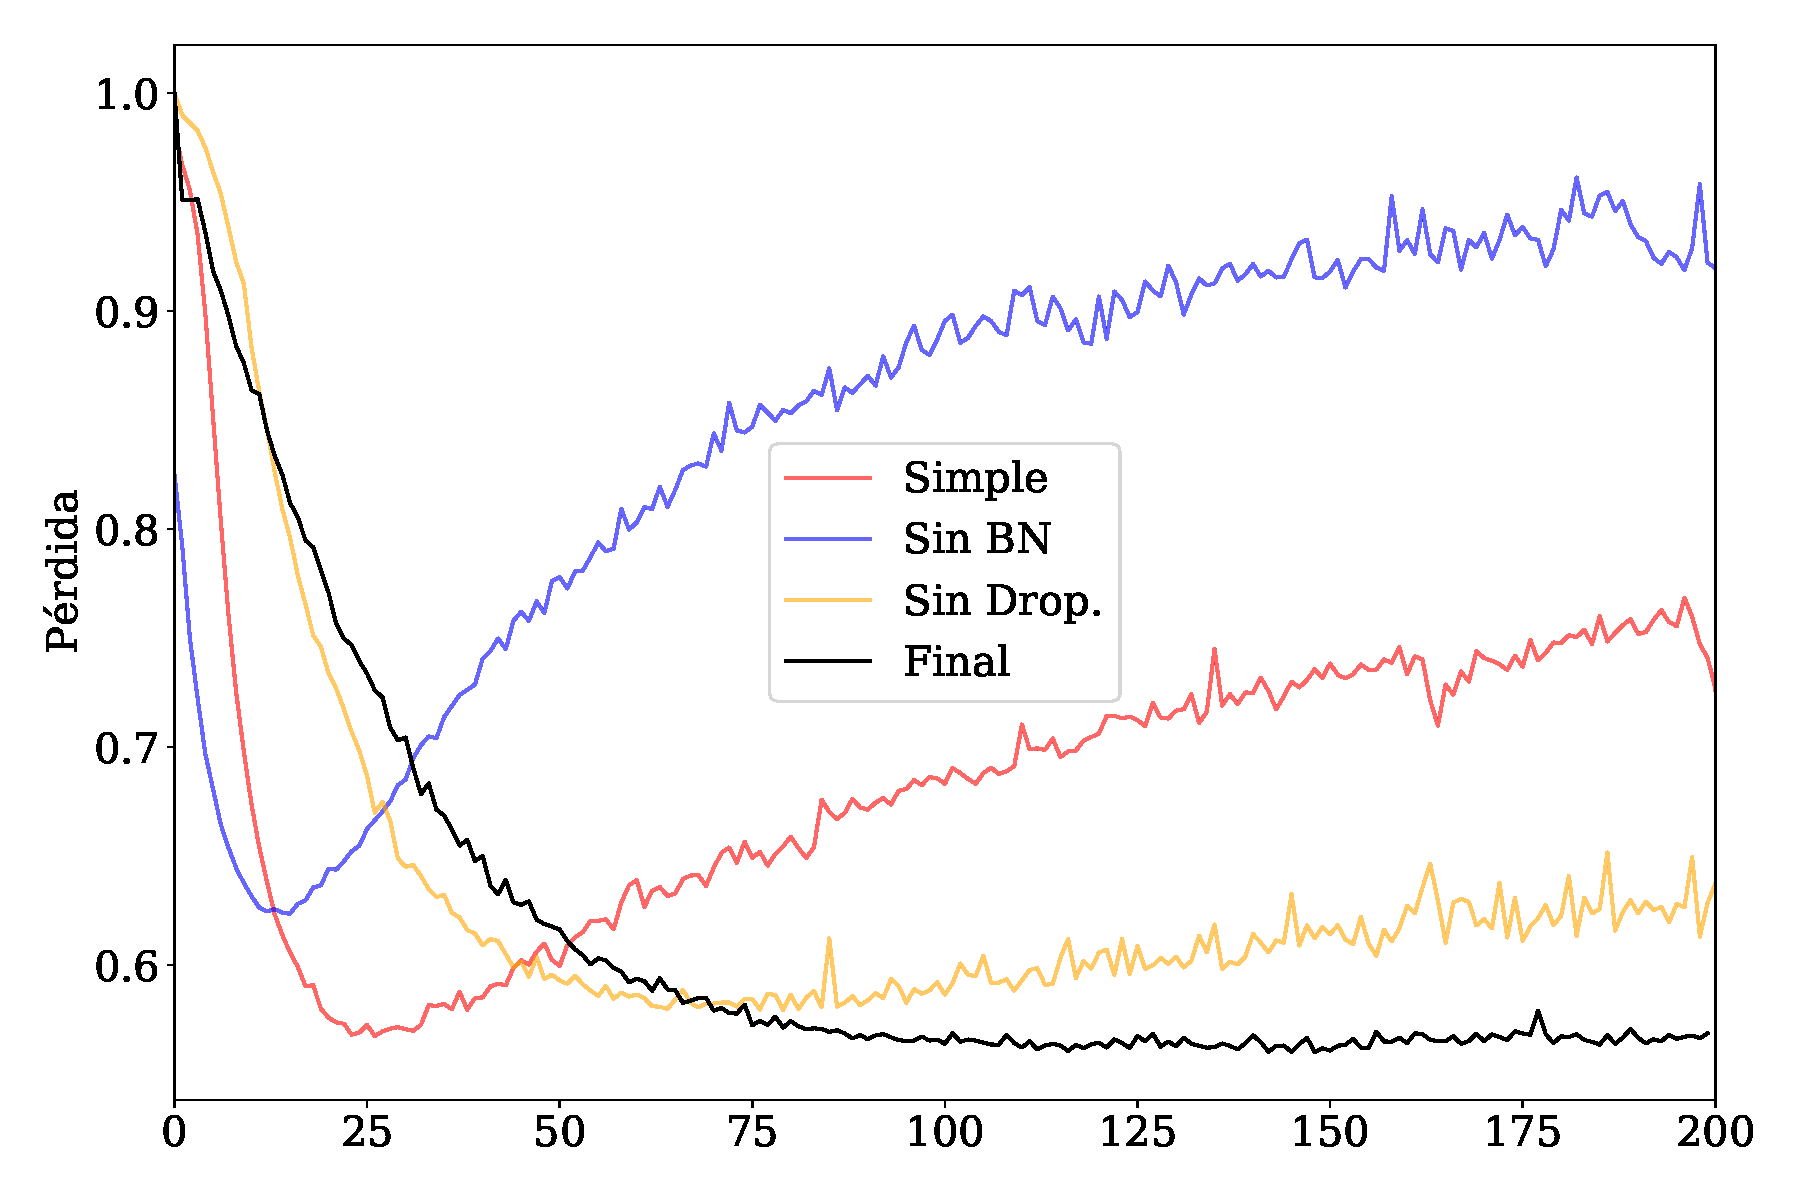
\includegraphics[width=0.5\textwidth]{Graphs/ejer3_loss_trails.pdf}
        \end{center}
        \caption{Pérdida normalizada con respecto al máximo en función de las épocas para distintas redes. Todas las redes, salvo la final, presentan overfitting. }
        \label{fig:ejer3_los_trails}
    \end{small}
\end{figure}




\section*{Ejercicio 4}

    En este apartado usamos redes convolucionales para resolver el problema anterior, esta red  tiene una capa de \emph{embedding} usada en procesamiento de lenguaje natural. Para utilizar esta capa definimos el tamaño máximo de reseña de $400$ palabras y la cantidad de palabras consideradas $max_words=10\,000$. La capa embedding permite que en vez de tener $25\,000$ vectores con $10\,000$ entradas para identificar las palabras utilizadas como en el caso de la red densa, ahora tenemos $25\,000$ vectores con $50$  entradas. La red entrena para hacer la transformación óptima para bajar las dimensión del problema en la red convolucional.

    A continuación se presenta con más detalles la red convolucional utilizada:
    \begin{verbatim}
    _____________________________________________
    Layer (type)         Salida      Parámetros   
    ============================================
    Embedding           (400, 50)    500000    
    ____________________________________________
    Dropout(0.5)        (400, 50)    0         
    ____________________________________________
    Conv1D              (400, 16)    3216      
    ____________________________________________
    MaxPooling1D        (200, 16)    0         
    ____________________________________________
    Dropout (0.5)       (200, 16)    0         
    ____________________________________________
    Flatten             (3200)       0         
    ____________________________________________
    Dense               
    Activación: relu    (30)         96030     
    Regul.: L2(0.01)
    ____________________________________________
    Dense
    Act.: Sigmoide      (1)          31    
    Regul.: L2(0.01)    
    ============================================
    Total params: 599,277
    \end{verbatim}

    Esta red convolucional tiene menos parámetros que la red densa, además   usando capas convolucionales se obtiene una precisión del $89.1\%$ como se puede observar en  la Fig.\ref{fig:ejer4_acc}, obteniendo una mejor precisión que la red densa.

    \begin{figure}[H]
        \begin{small}
            \begin{center}
                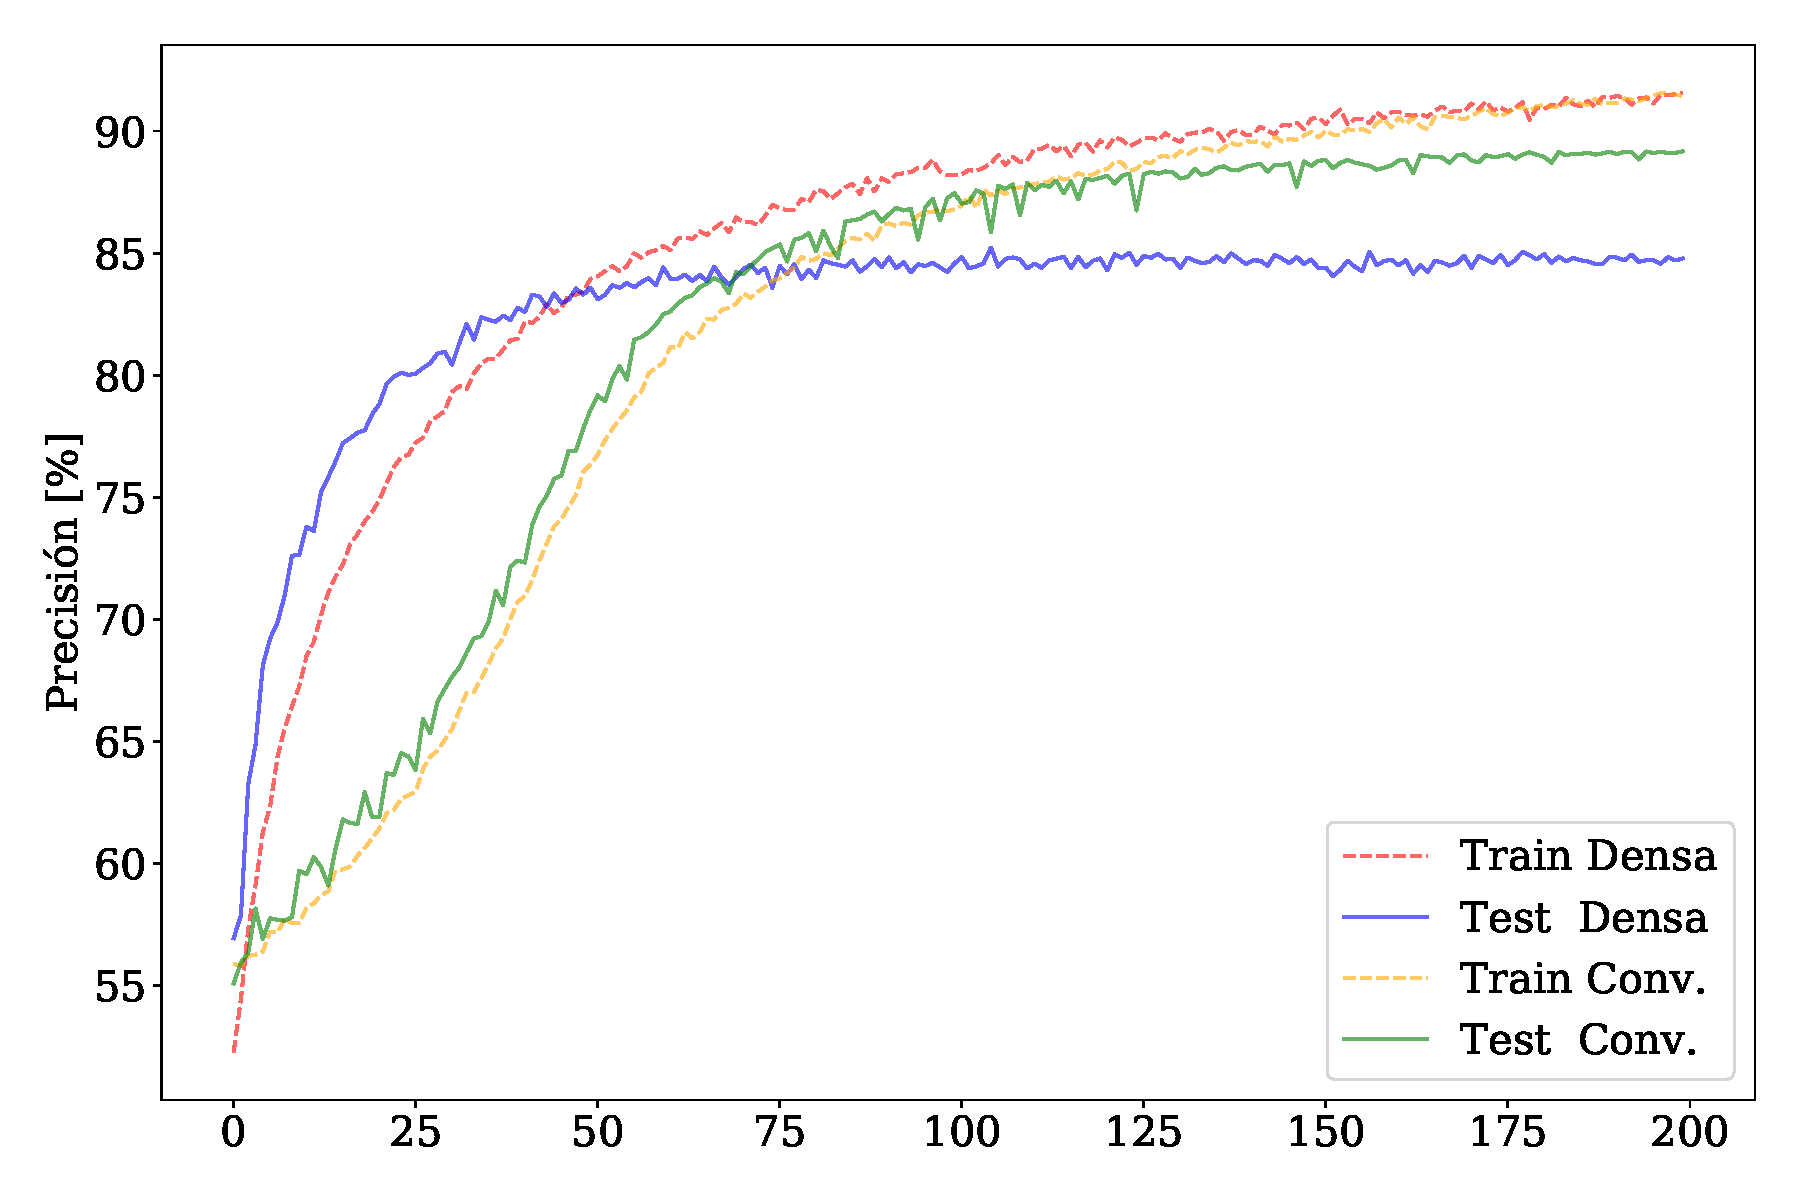
\includegraphics[width=0.5\textwidth]{Graphs/ejer4_acc.pdf}
            \end{center}
            \caption{Precisión de la red en función de las épocas}
            \label{fig:ejer4_acc}
        \end{small}
    \end{figure}


    \begin{figure}[H]
        \begin{small}
            \begin{center}
                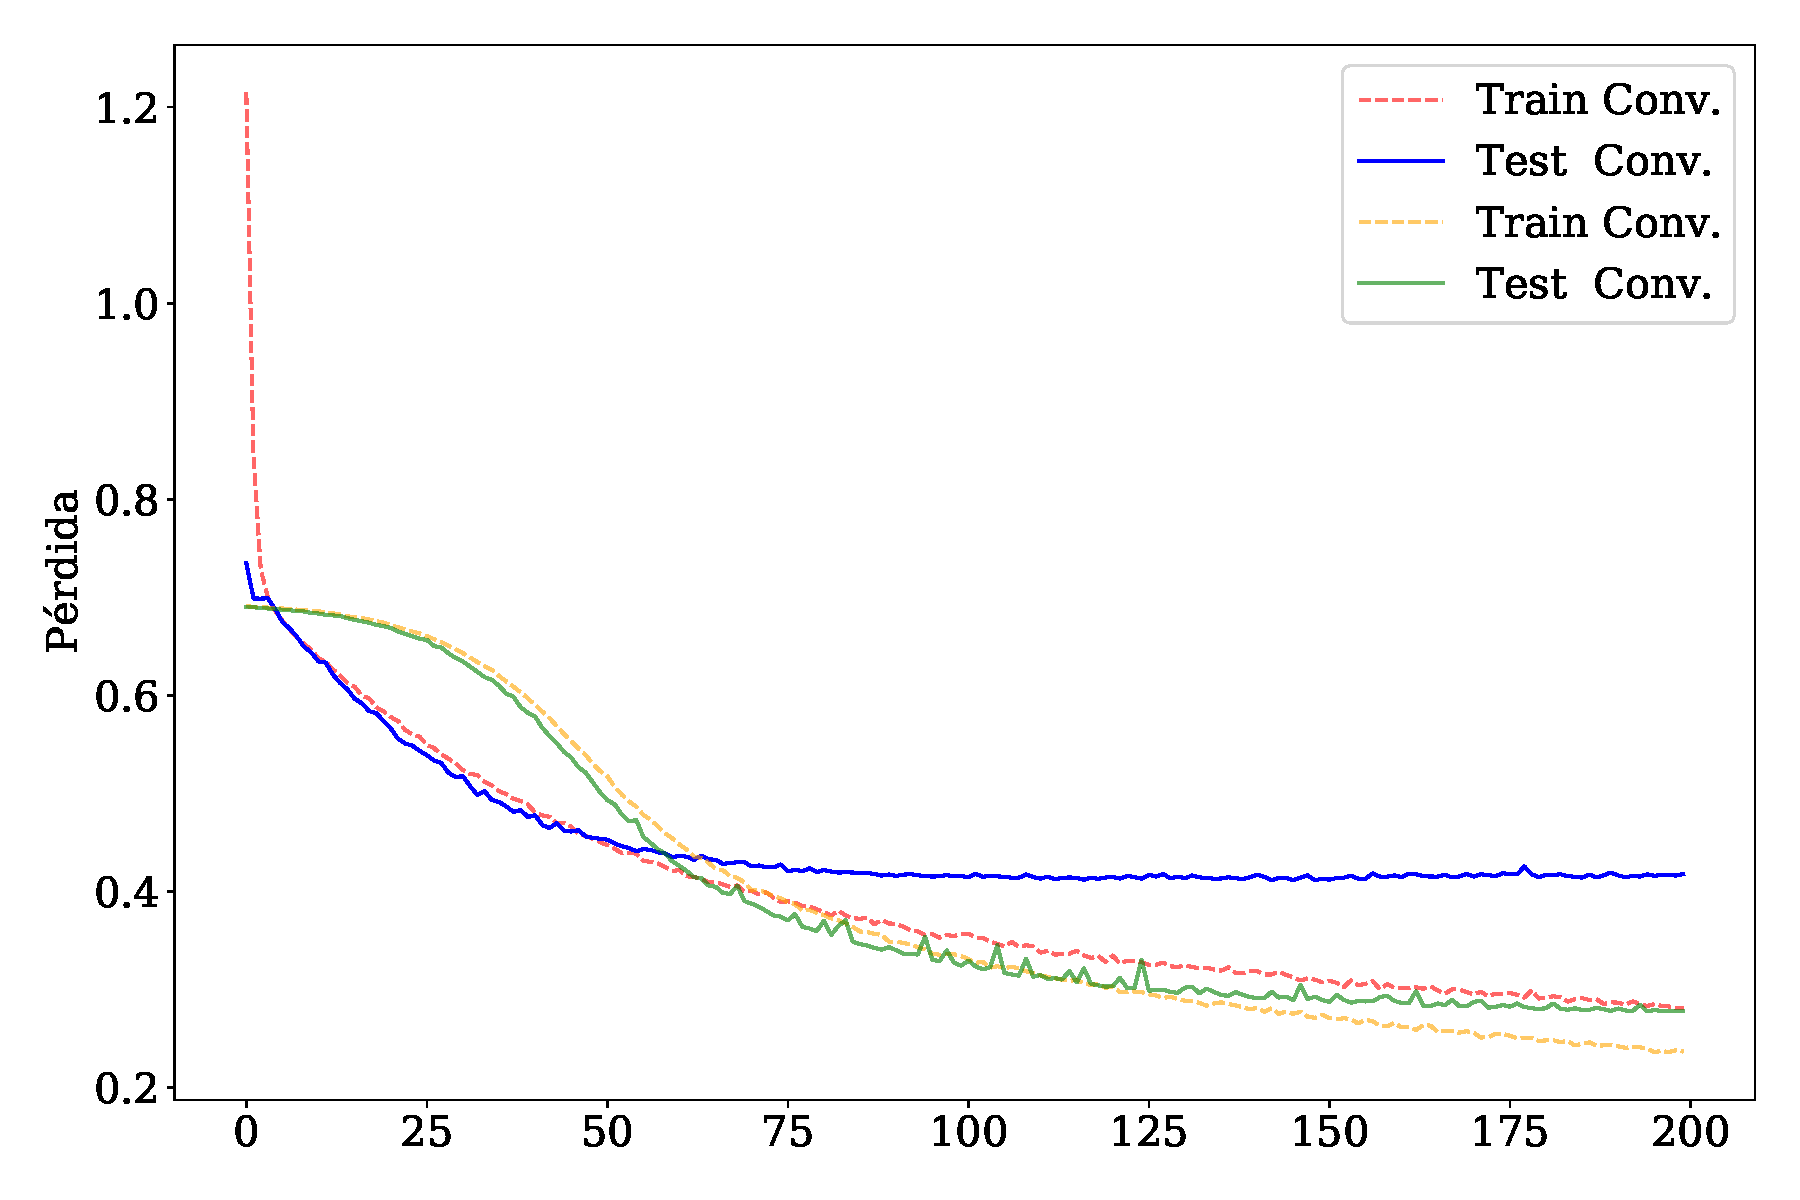
\includegraphics[width=0.5\textwidth]{Graphs/ejer4_loss.pdf}
            \end{center}
            \caption{Pérdida normalizada con respecto al máximo en función de las épocas. }
            \label{fig:ejer4_loss}
        \end{small}
    \end{figure}



\section*{Ejercicio 5}

    El mapeo logístico es una función del tipo $x(t+1) = r x(t)(1-x(t))$, conocida por presentar caos dependiendo del valor de r. Se dice que una función tiene un comportamiento caótico si dos valores iniciales  cercanos, la diferencia entres las salidas de los mismo crece exponencialmente con la cantidad de iteraciones.  En este ejercicio el mapeo logístico tiene un valor $r=4$ donde se presenta un comportamiento caótico salvo algunos números. 

    Podemos hacer una red para los siguientes dos escenarios:
    \begin{enumerate}
        \item Podemos hacer que la red aprenda la función $f(x)= 4x(1-x)=4x-4x^2$
        \item Podemos intentar que la red aprenda el comportamiento caótico del mapeo logístico entrenándola con un conjunto de $\{ x(0), t\}$ distintos.
    \end{enumerate}

    \subsection*{Escenario 1}
    La red tiene como objetivo aprender la función $f(x)= 4x(1-x)=4x-4x^2$, para eso se entrena con números en el rango  $[0,1]$ como entrada y como salida esperada $f([0,1])$.

    En este caso se cambio la cantidad de ejemplos de entrenamiento, donde la cantidad de ejemplos de validación es la mitad de los ejemplos de entrenamiento. En la Fig.\,\ref{ejer5} se muestra la pérdida normalizada con respecto al mayor valor, para distintas cantidades de ejemplos. Se puede ver que para $10$ ejemplos de entrenamiento y $5$ de validación, la red tiende a tener overfitting y en cambio para $(25,50)$ la red tiene una pérdida mayor que $(12, 24)$. En  varias ejecuciones, la red entrenada con $(25,50)$ también presentaba overfitting.

    \begin{figure}[H]
        \begin{small}
            \begin{center}
                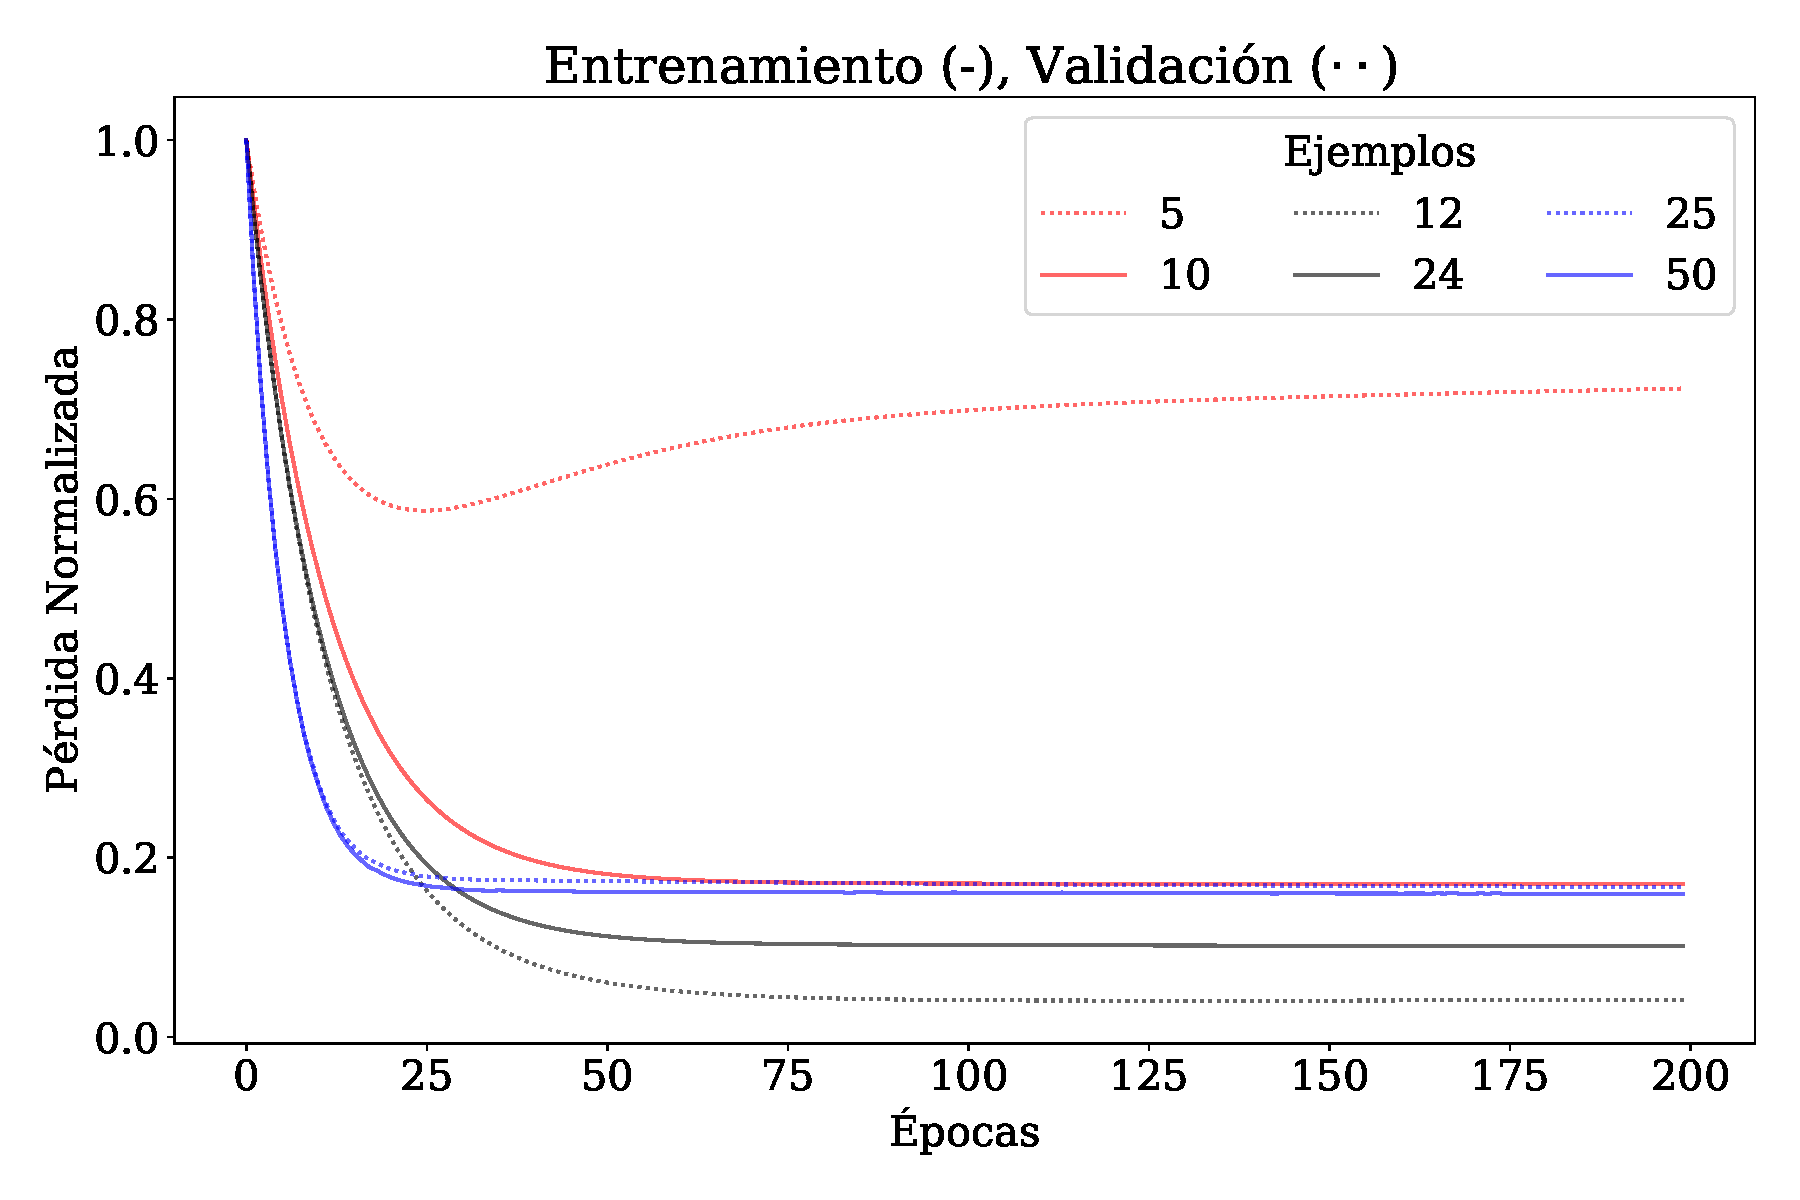
\includegraphics[width=0.5\textwidth]{Graphs/ejer5_los_gen.pdf}
            \end{center}
            \caption{Pérdida de la validación y entrenamiento para distintas cantidades de ejemplos.}
            \label{fig:ejer5}
        \end{small}
    \end{figure}


    \subsection*{Escenario 2}
    Este escenario no es realizable con la arquitectura que se pide, ya que la entrada debería tener dos dimensiones, una para $x(0)$ y otra para $t$.  Si entrenáramos a la red con un par $\{x(0), x(t)\}$ con $t$ cuales quiera, por el comportamiento caótico de la función, la red no puede predecir la salida que puede tener $x(0) + \epsilon$.

\section*{Ejercicio 6}

    En este ejercicio se implementa una red fully-connected para predecir si un paciente puede tener o no diabetes dado su historial médico. La base de datos utilizado es público y fue utilizado por primera vez en el siguiente trabajo \cite{pima}.

    Para algunos pacientes en este conjunto de datos se tiene información incompleta de su historial médico, por ejemplo un dato es la presión arterial que en algunos casos en 0. Dado que solo se tiene información de 768 pacientes, se optó por reemplazar los valores nulos por la media del resto de los pacientes las siguientes columnas: glucosa en sangre, presión arterial, insulina e indice de masa corporal.


    La red utilizada tiene la siguiente arquitectura:

    \begin{itemize}
        \item Capa de entrada.
        \item Capa oculta de 10 neuronas con función de activación lineal y con bias.
        Primeramente se usó una función de activación del tipo ReLU, pero se cambió por una lineal dado que la ReLU de mejores resultados. Esto puede  deberse a que la ReLU no aprende la correlación negativa que pueden tener dos aspectos del historial médico.  

        Se utilizó 10 neuronas para que la red aprenda las posibles correlaciones entre los datos del historial clínico. Para lograr esto la capa oculta tiene que tener al menos 8 neuronas, se optó por 10 porque funcionaba y por encima de 10 la red puede tener parámetros redundantes. También se probó agregando una capa más pero la red no mejoró su rendimiento

        \item Capa de salida con activación ReLU: Se optó por una ReLU por encima de la lineal porque se espera que la salida sea 0 sí la red predice que no va a desarrollar diabetes, y 1 en caso contrario. También se utilizó un función sigmoidal pero la red presentaba un overfitting, incluso con la regularización. Se utilizó el optimizador SGD con una tasa de aprendizaje de 0.001 con la función de pérdida  
    \end{itemize}

    Para verificar que la red tiene capacidad de generalización dada la cantidad de datos, se usó el método k-fold de la siguiente manera: se toma el conjunto de datos y se separa el conjunto de entrenamiento y validación $5$ veces y se entrena la red para cada vez. Esto se implementó con el módulo \verb|model_selection.KFold| de  \verb|sklearn|. En cada iteración, el conjunto de entrenamiento y validación tenían entre $614-615$ y $154-153$ pacientes respectivamente, y los pesos del entrenamiento anterior no se tienen en cuenta. 

    El preprocesado de los datos se realizó en cada entrenamiento, el mismo consistió en resta los datos por la media y dividir por la desviación estándar.

    En las  Figs \ref{fig:ejer6_acc} y \ref{fig:ejer6_loss} de presentan la media de la precisión y pérdida para vez que se entrena la red. Para tener una referencia de como varían en cada entrenamiento en función de las épocas,  se muestra  la desviación estándar en cada época con el sombreado alrededor de la línea más oscura. Se observó que no se corrigen los datos nulos la red tiene una precisión similar a lo obtenido realizando la corrección, los resultados se muestran en las Figs. \ref{fig:ejer6_acc_raw} y \ref{fig:ejer6_loss_raw}. La diferencia principal es que la variación de la precisión media es menor con la corrección.

    \begin{figure}[H]
        \begin{small}
            \begin{center}
                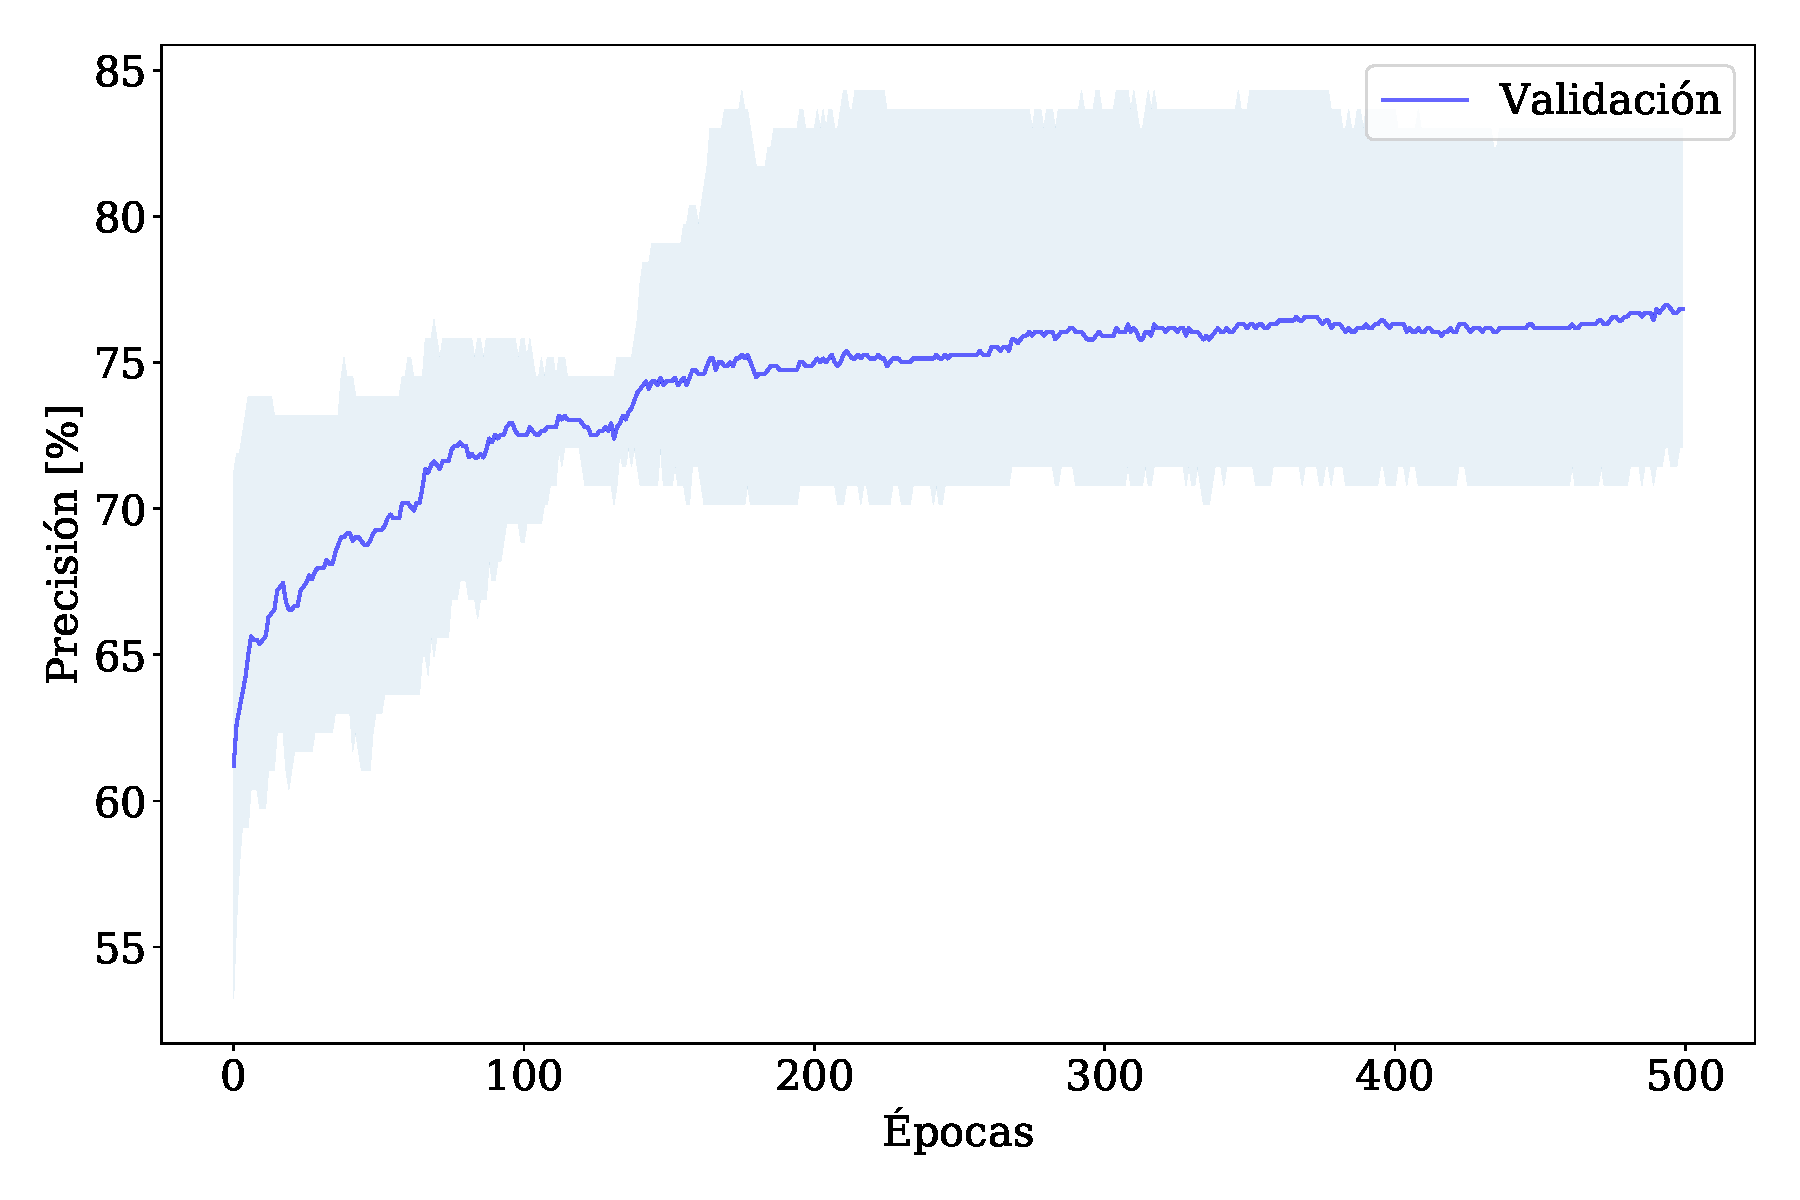
\includegraphics[width=0.46\textwidth]{Graphs/ejer6_acc.pdf}
            \end{center}
            \caption{Precisión de la red en función de las épocas. Se muestra una estimación del error de la precisión por época. La precisión media alcanza un valor de $77.2\%$}
            \label{fig:ejer6_acc}
        \end{small}
    \end{figure}


    \begin{figure}[H]
        \begin{small}
            \begin{center}
                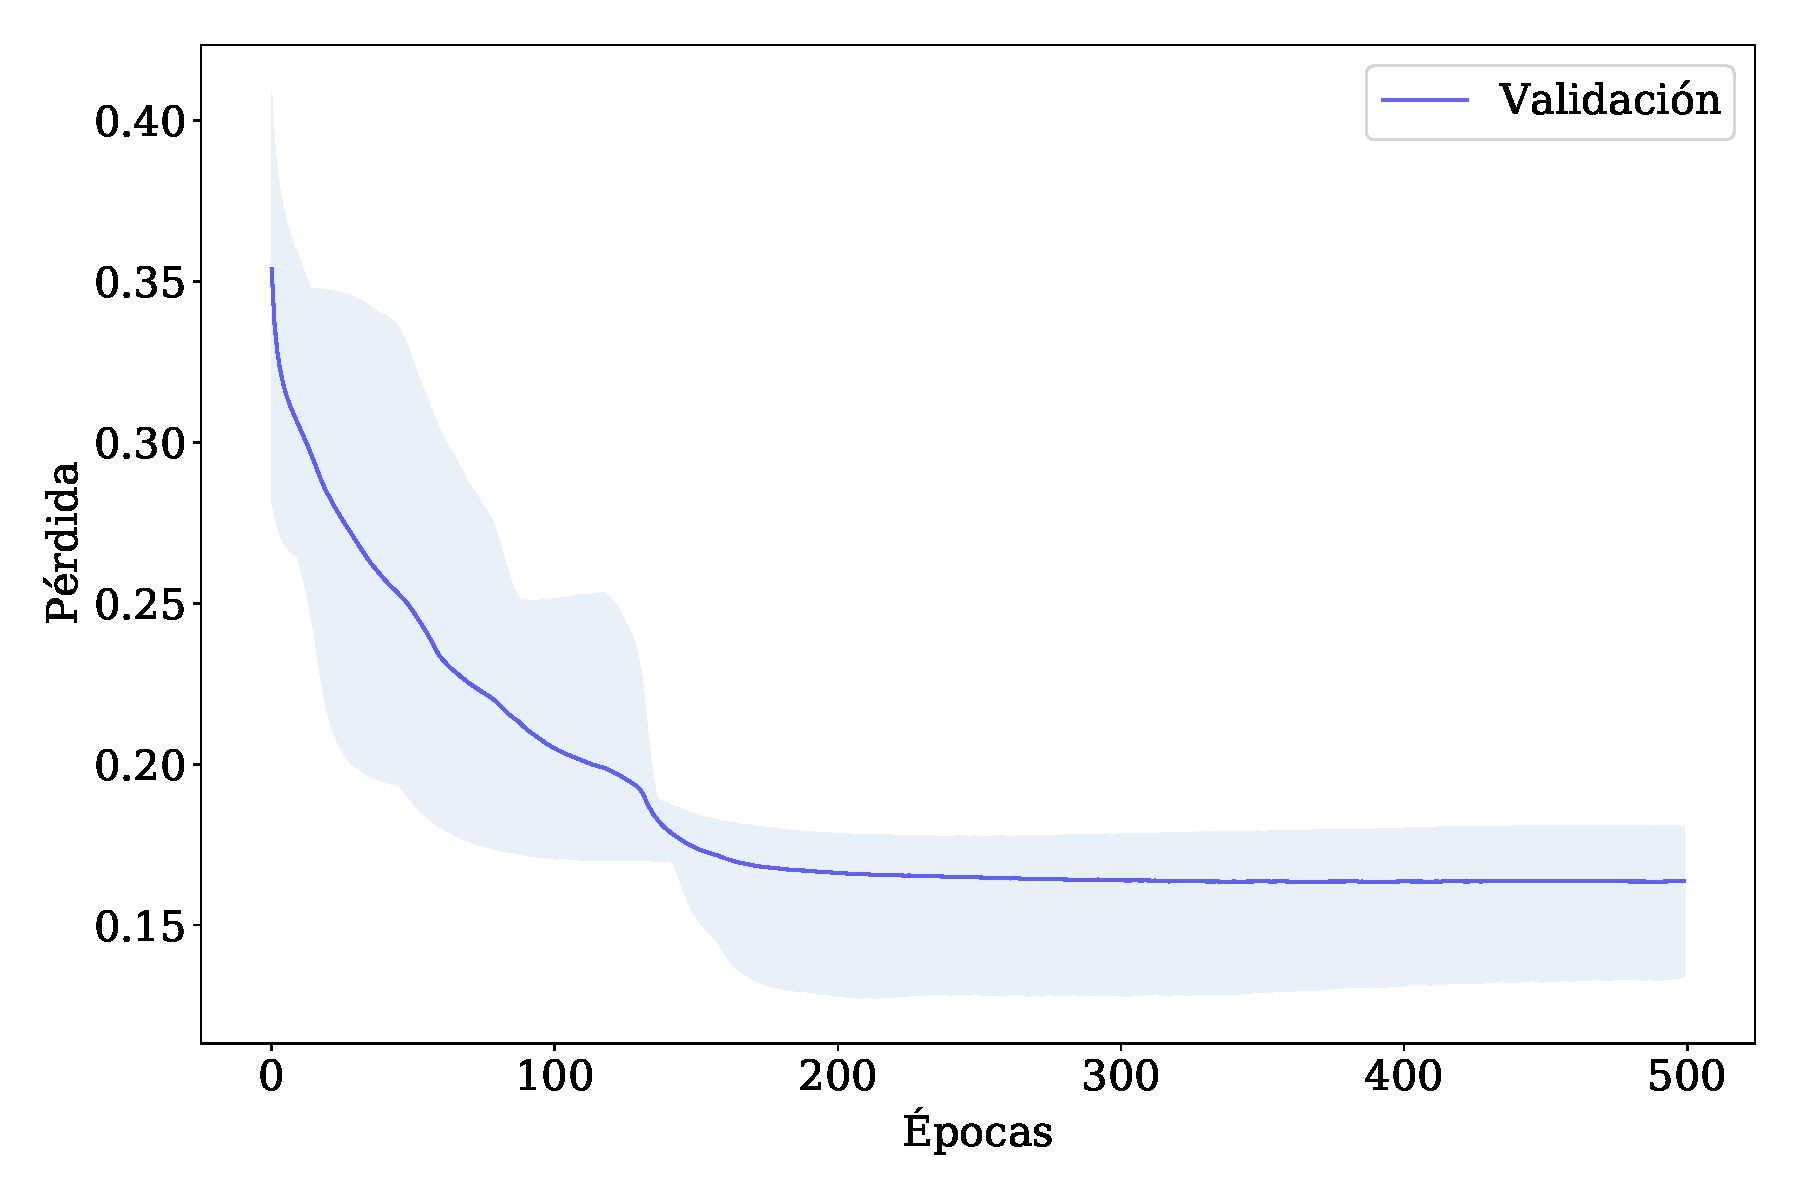
\includegraphics[width=0.5\textwidth]{Graphs/ejer6_loss.pdf}
            \end{center}
            \caption{Pérdida de la red en función de las épocas. Se muestra una estimación del error de la precisión por época.}
            \label{fig:ejer6_loss}
        \end{small}
    \end{figure}

    \begin{figure}[H]
        \begin{small}
            \begin{center}
                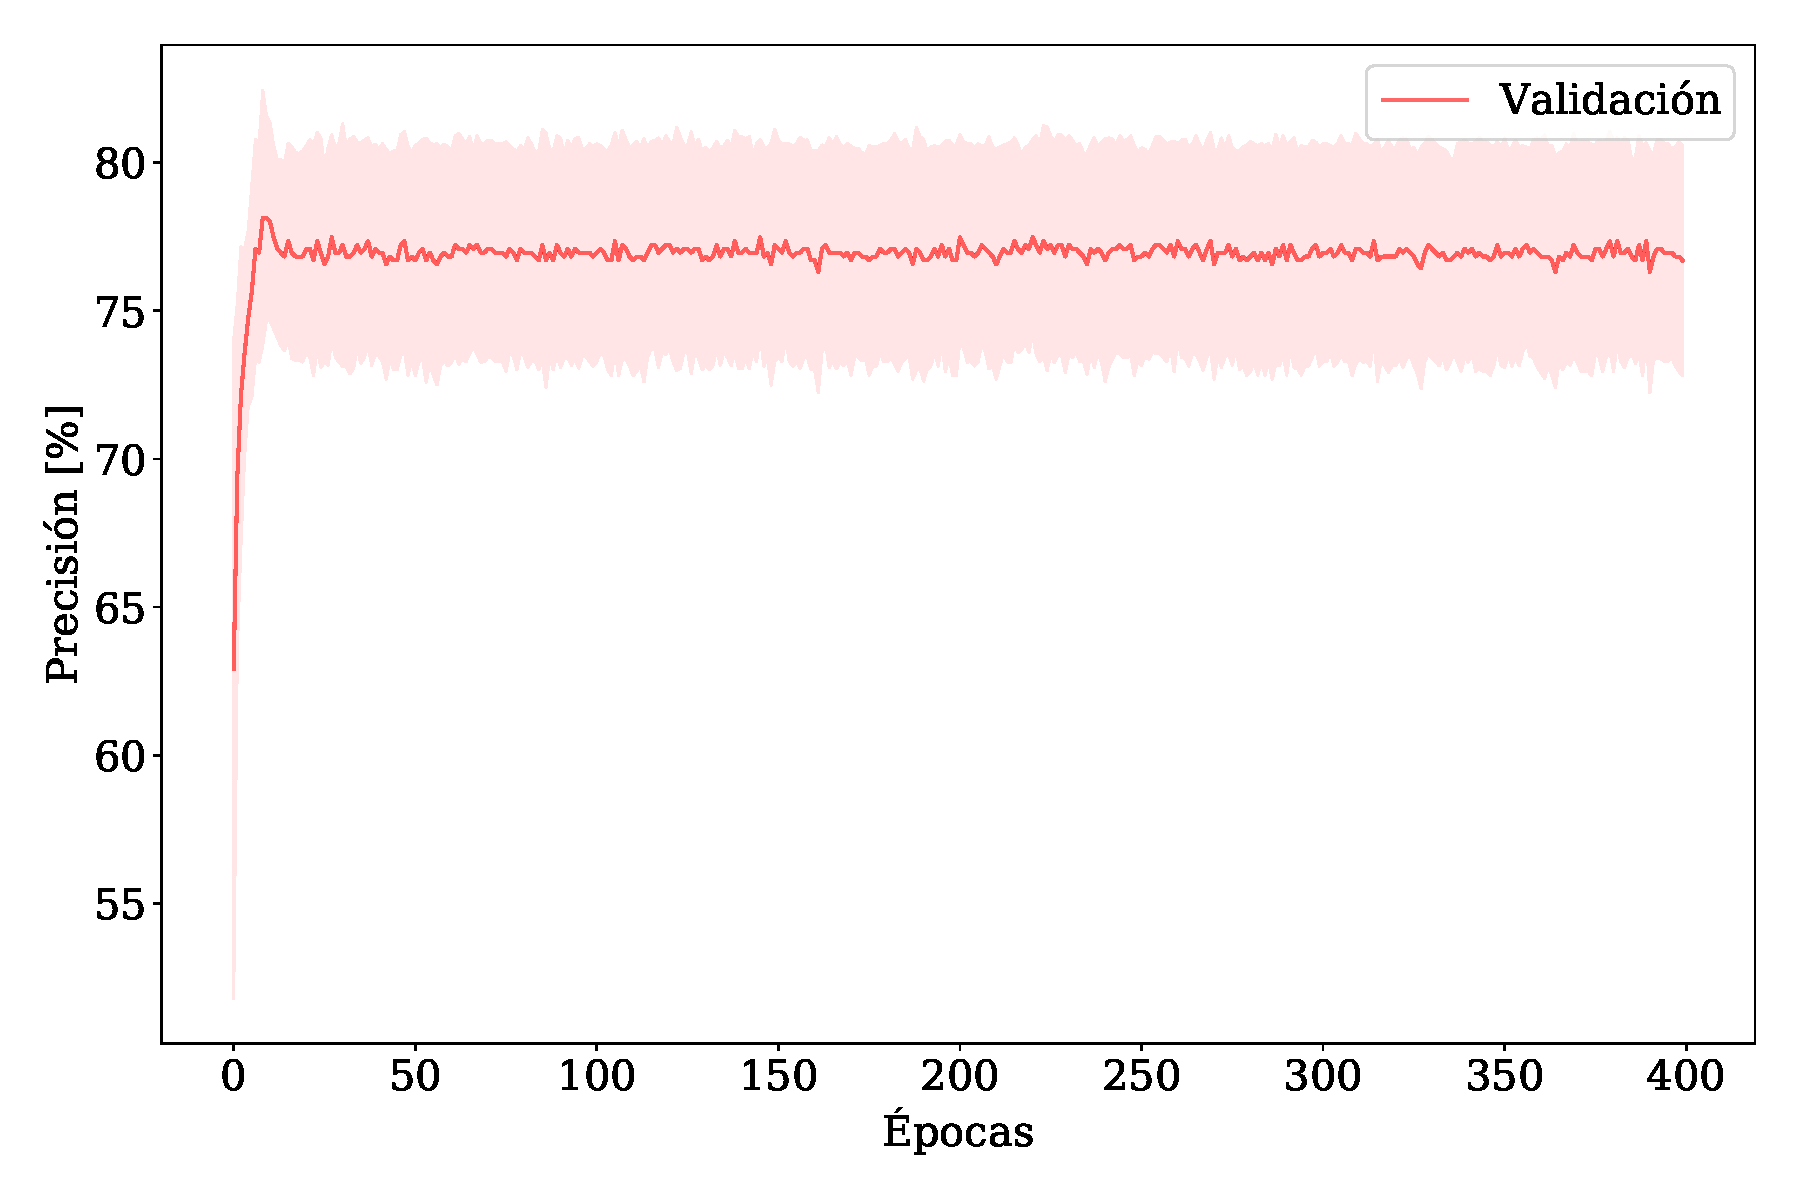
\includegraphics[width=0.5\textwidth]{Graphs/ejer6_acc_raw.pdf}
            \end{center}
            \caption{Precisión de la red en función de las épocas con los datos sin corrección.}
            \label{fig:ejer6_acc_raw}
        \end{small}
    \end{figure}




\section*{Ejercicio 7}

    En este ejercicio se implementa una red con capas convolucionales  para eliminar el ruido de la imágenes de los dígitos del MNIST. Para esto se implementó un autoencoder que toma como entrada la imagen  con ruido y como salida se tiene la imagen sin el ruido. Para lograr esto la red tiene dos etapas: \emph{encoding} y \emph{decoding}. El \emph{encoding} toma la imagen de $28\times28\times1$ con un único canal de color y la lleva hasta una imagen de $7\times7\times32$. Mientras que en el \emph{decoding} se lleva la imagen de $7\times7\times32$ a una imagen de $28\times28\times1$.   Se modificó las dimensiones de la imagen del encoding a 8 y 16 para disminuir la cantidad de parámetros pero no obtuvo la mejor resolución con 32.

    \begin{figure}[H]
        \begin{small}
            \begin{center}
                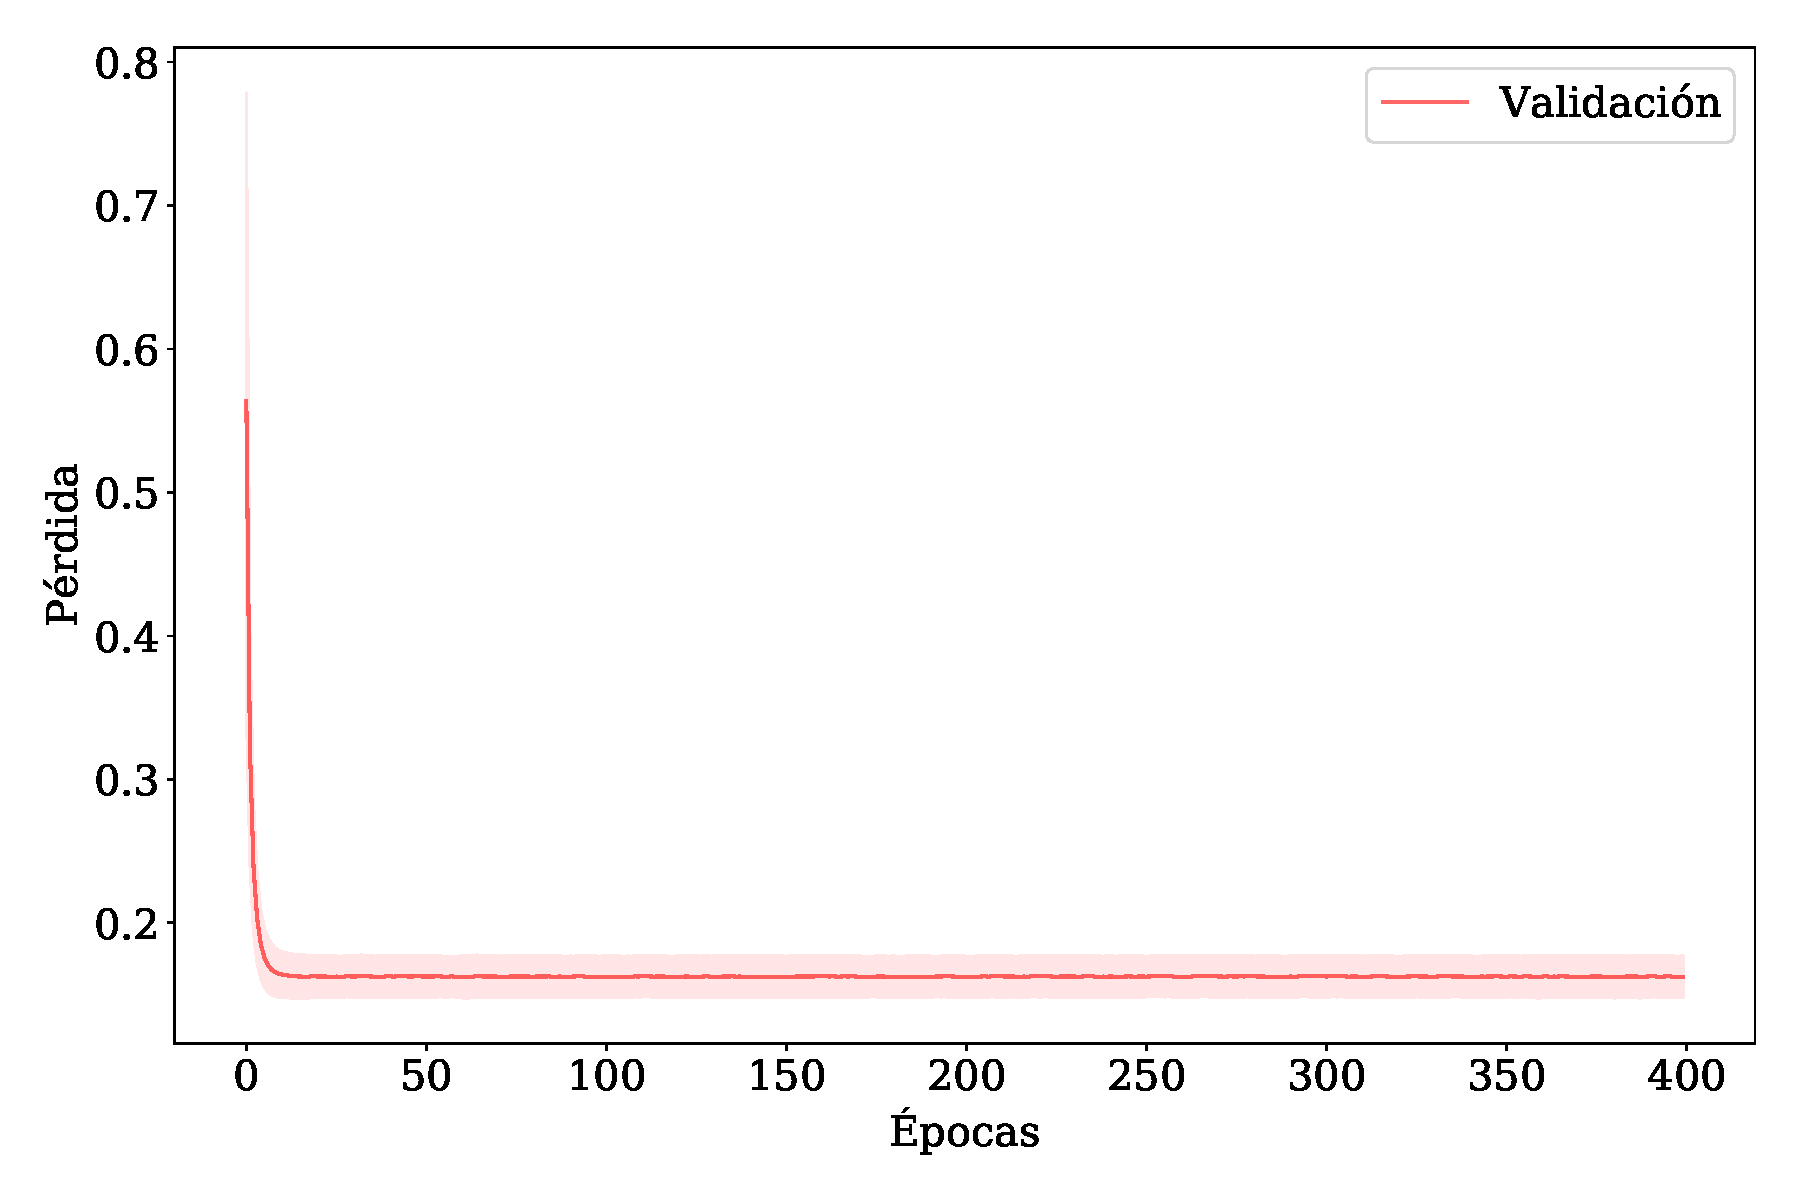
\includegraphics[width=0.5\textwidth]{Graphs/ejer6_loss_raw.pdf}
            \end{center}
            \caption{Pérdida de la red en función de las épocas con los datos sin corrección. }
            \label{fig:ejer6_loss_raw}
        \end{small}
    \end{figure}

    El optimizador utilizado fue el \emph{adam} con una tasa de aprendizaje de 0.001, se probó con SGD pero se obtuvo mejores resultados con la primera. La función de pérdida utilizada fue \verb|CCE| por lo que la capa de salida fue una sigmoidal. La capas ocultas tiene funciones de activación ReLU porque las imágenes tienen un valor entre 0 y 1.


    En las Figs. \ref{fig:ejer7_acc} y \ref{fig:ejer7_loss} se observan la precisión y pérdida en función de las épocas. Para mostrar un ejemplo del uso de esta red, en la Fig.\ref{fig:ejer7} se muestra un ejemplo de ejemplos de validación con el ruido y luego de ser filtradas por la red entrenada. Se observa que el ruido de la imagen del dígito disminuye notablemente.

    \begin{figure}[H]
        \begin{small}
            \begin{center}
                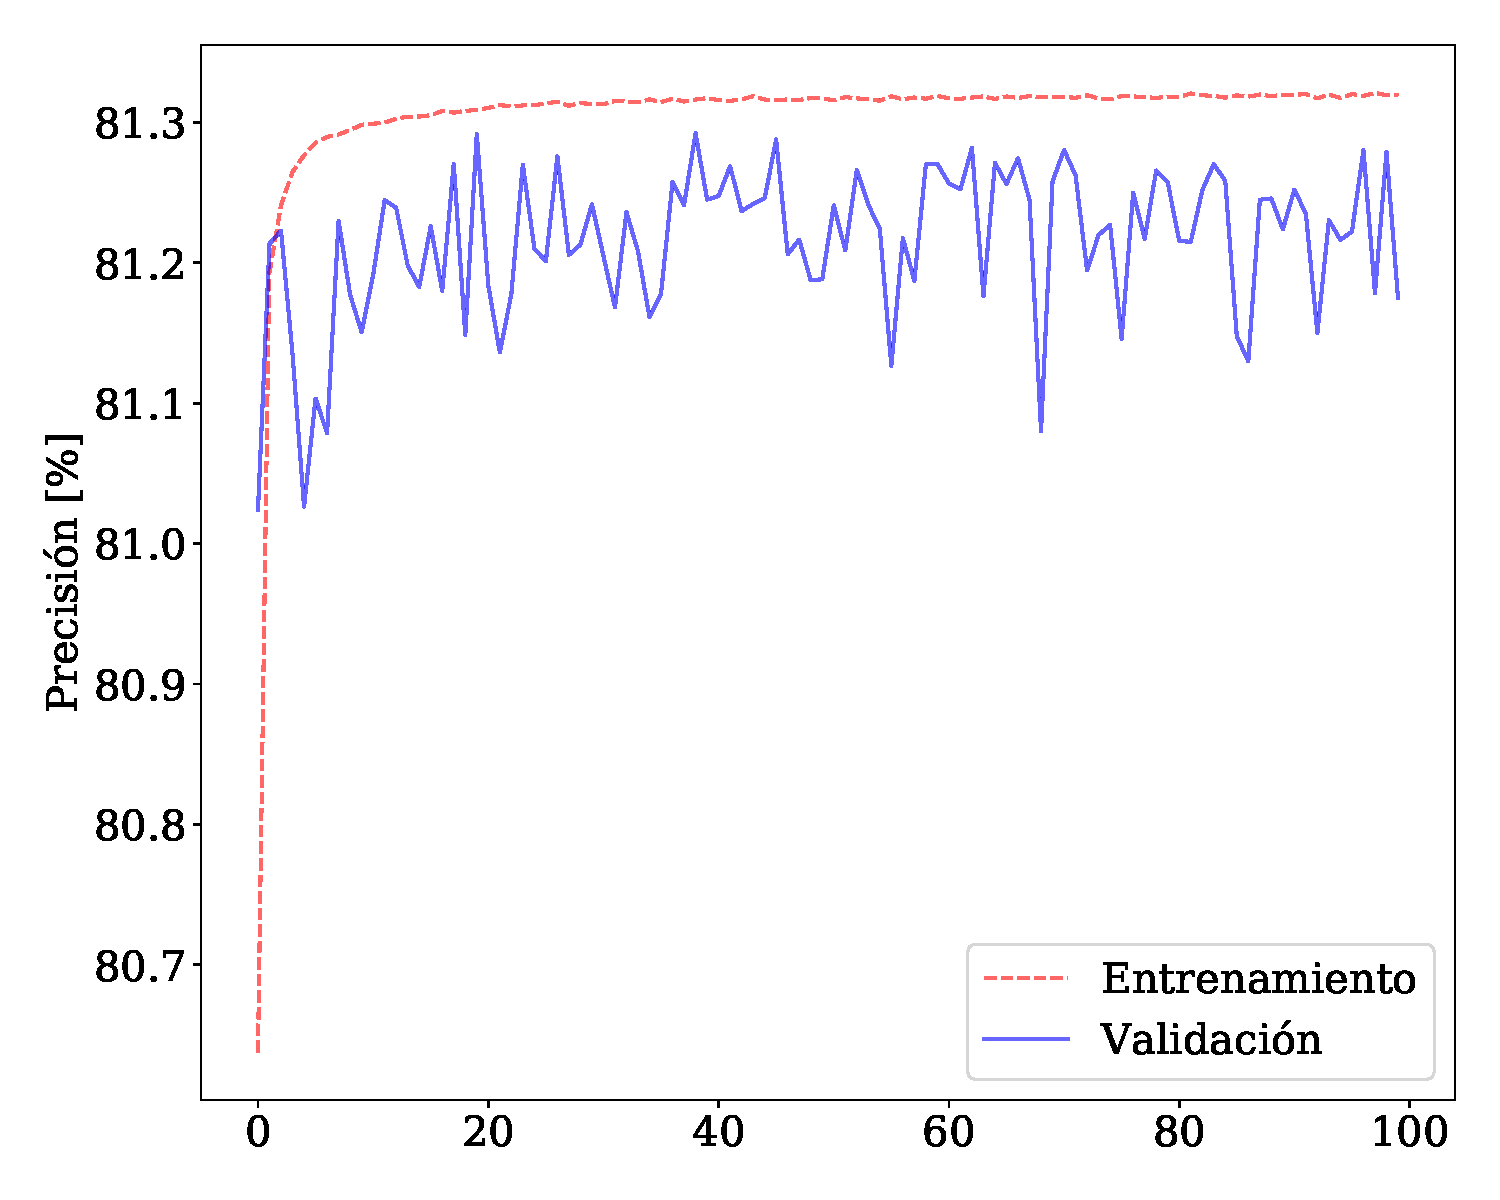
\includegraphics[width=0.5\textwidth]{Graphs/ejer7_acc.pdf}
            \end{center}
            \caption{Precisión de la red en función de las épocas. Se alcanza un precisión del 81.2 \% con el conjunto de validación}
            \label{fig:ejer7_acc}
        \end{small}
    \end{figure}


    \begin{figure}[H]
        \begin{small}
            \begin{center}
                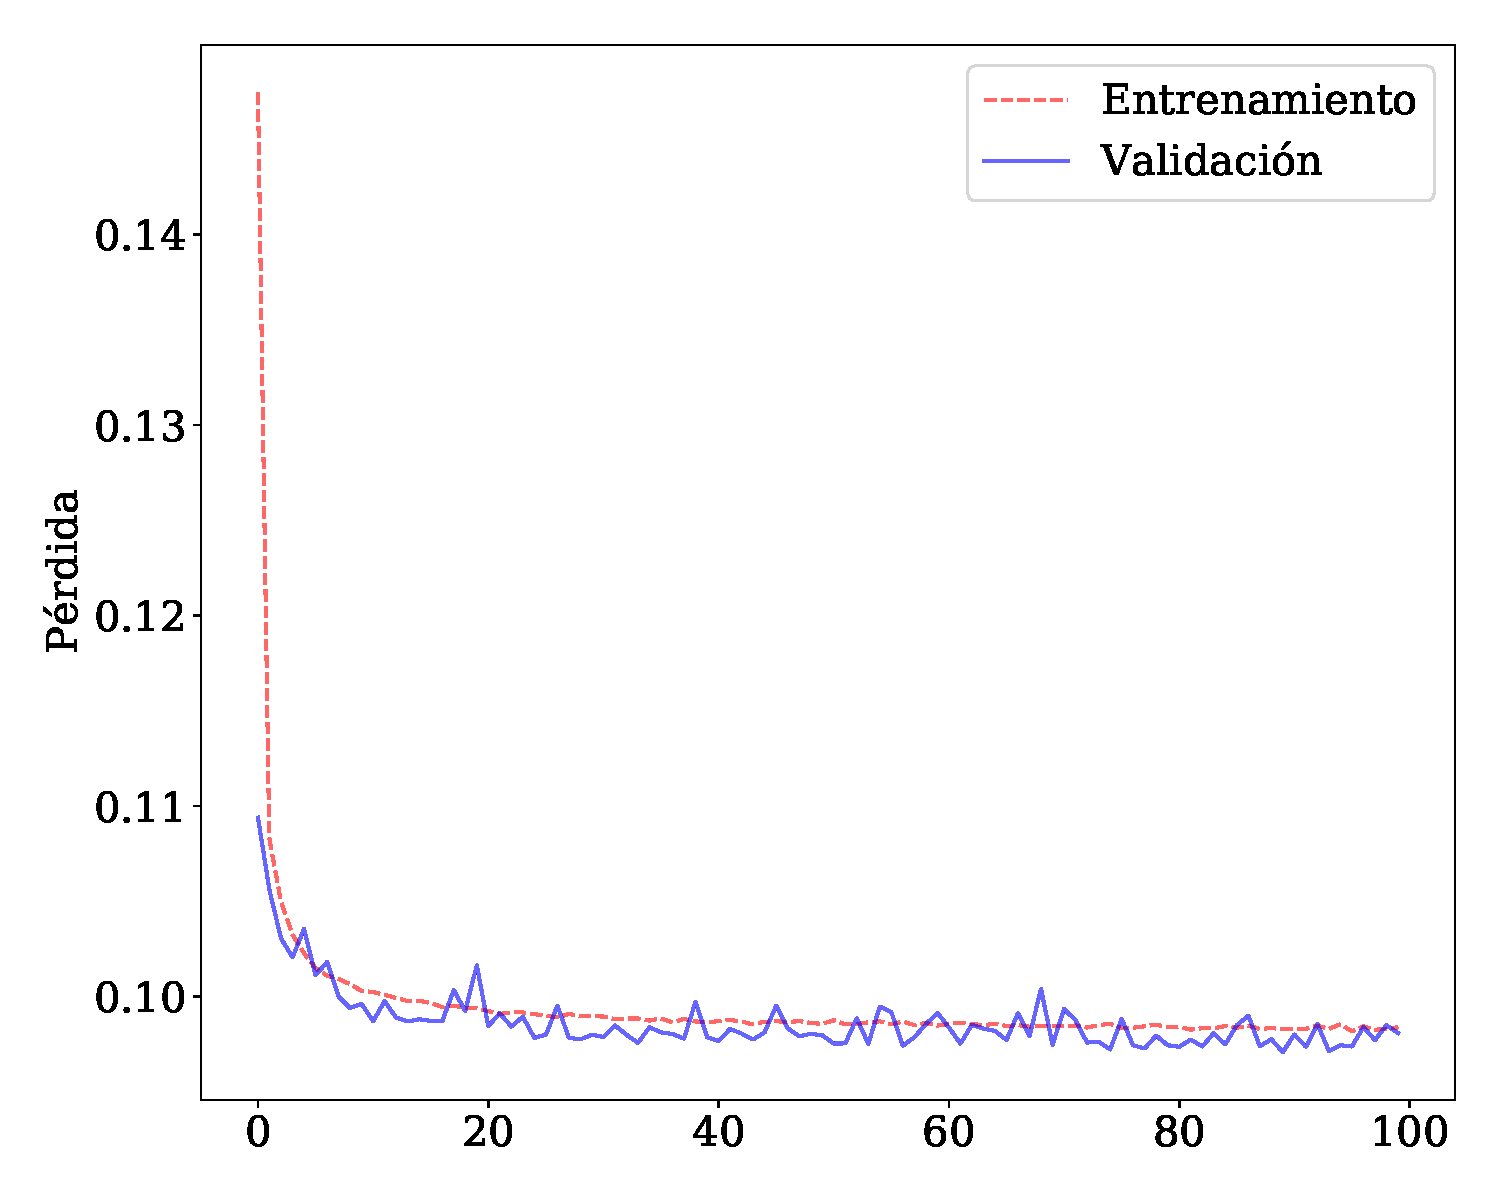
\includegraphics[width=0.45\textwidth]{Graphs/ejer7_loss.pdf}
            \end{center}
            \caption{Pérdida de la red en función de las épocas. }
            \label{fig:ejer7_loss}
        \end{small}
    \end{figure}


    \begin{figure}[H]
        \begin{small}
            \begin{center}
                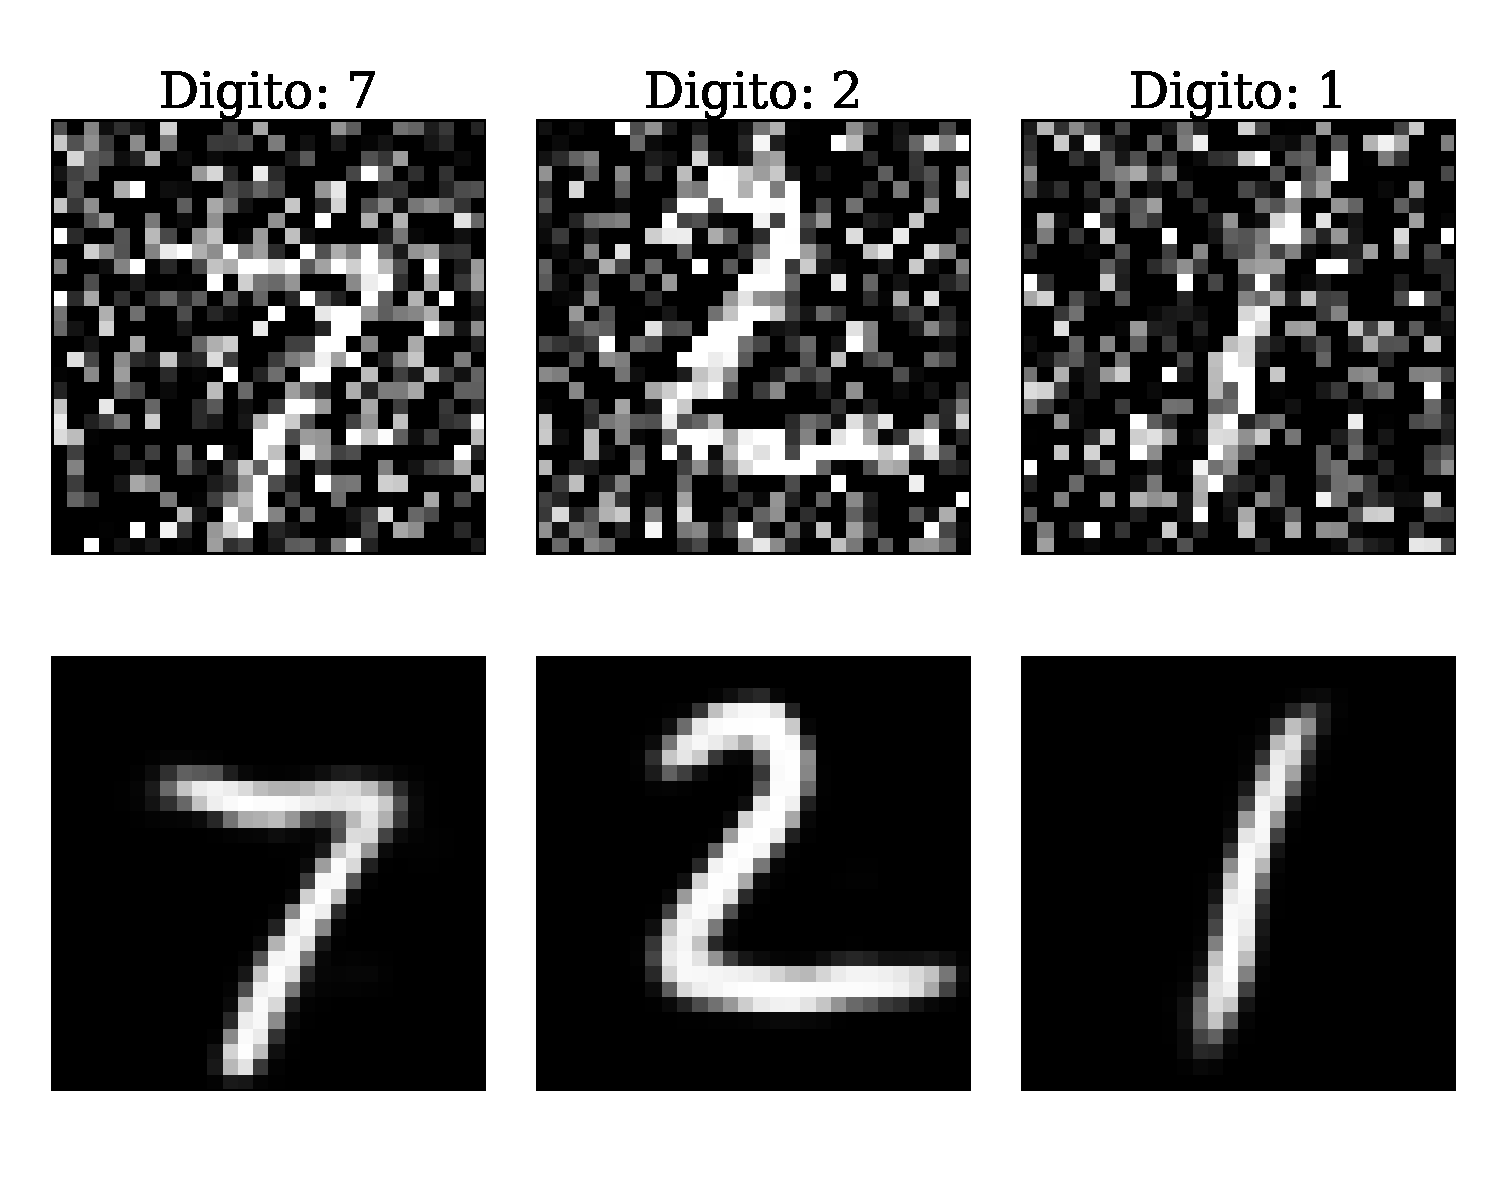
\includegraphics[width=0.45\textwidth]{Graphs/ejer7.pdf}
            \end{center}
            \caption{Ejemplo de entrada y salida de la red posterior al entrenamiento. Se observa que el ruido se reduce y se obtiene una imagen clara del dígito en cuestión.}
            \label{fig:ejer7}
        \end{small}
    \end{figure}


\section*{Ejercicio 8}

    En este ejercicio se busca clasificar la base de datos de las imágenes de dígitos del MNIST. Se implementaron dos tipos de redes: densa y convolucional. La red dense tiene una arquitectura similar a la utilizada para clasificar las imágenes de CIFAR-10. Como se muestra a continuación:

    \begin{verbatim}
    Layer           Salida        Parámetros   
    =========================================
    Dense (ReLU)    (100)         78500     
    _________________________________________
    Dense (Softmax) (10)          1010      
    \end{verbatim}
    que tiene un total de  $79\,510$ parámetros. Para la red convolucional se usaron capas convolucionales y  de Max Pooling, además de capa Dropout donde ignoramos un $20\%$ de la entrada a esa capa. Esta capa es utilizada para aumentar la generalización de la red evitando el overfitting. La lista a continuación tiene más detalles de la red:
    \begin{verbatim}
    Layer           Salida         Parámetros
    =========================================
    Conv2D          (24, 24, 30)   780     
    _________________________________________
    MaxPooling2D    (12, 12, 30)   0       
    _________________________________________
    Conv2D          (10, 10, 10)   2710    
    _________________________________________
    MaxPooling2D    (5, 5, 10)     0       
    _________________________________________
    Dropout (0.2)   (5, 5, 10)     0       
    _________________________________________
    Flatten         (250)          0       
    _________________________________________
    Dense (Softmax) (10)           2510    
    =========================================
    Total parámetros: 6,000
    \end{verbatim}

    Se utilizó el optimizador SGD con una tasa de aprendizaje de 0.001, también se probó utilizando el optimizador  adam pero la red tenía a tener overfitting en la red densa, incluso con una función de regularizador con parámetro de $0.1$. La función de pérdida es CCE y la última capa en ambas redes en densa con una activación softmax.

    En las Figs. \ref{fig:ejer8_acc} y \ref{fig:ejer8_loss} se muestran las curvas de precisión y pérdida normalizada para los datos de entrenamiento y validación para las redes mencionadas. La red convolucional tiene una mejor precisión final de $97.9\%$ en el conjunto de validación con respecto a la densa que alcanza un $93.67\%$. Otra diferencia importante es la cantidad de parámetros de las redes, la red densa utiliza  13 veces más parámetros de la red convolucional.
    \begin{figure}[H]
        \begin{small}
            \begin{center}
                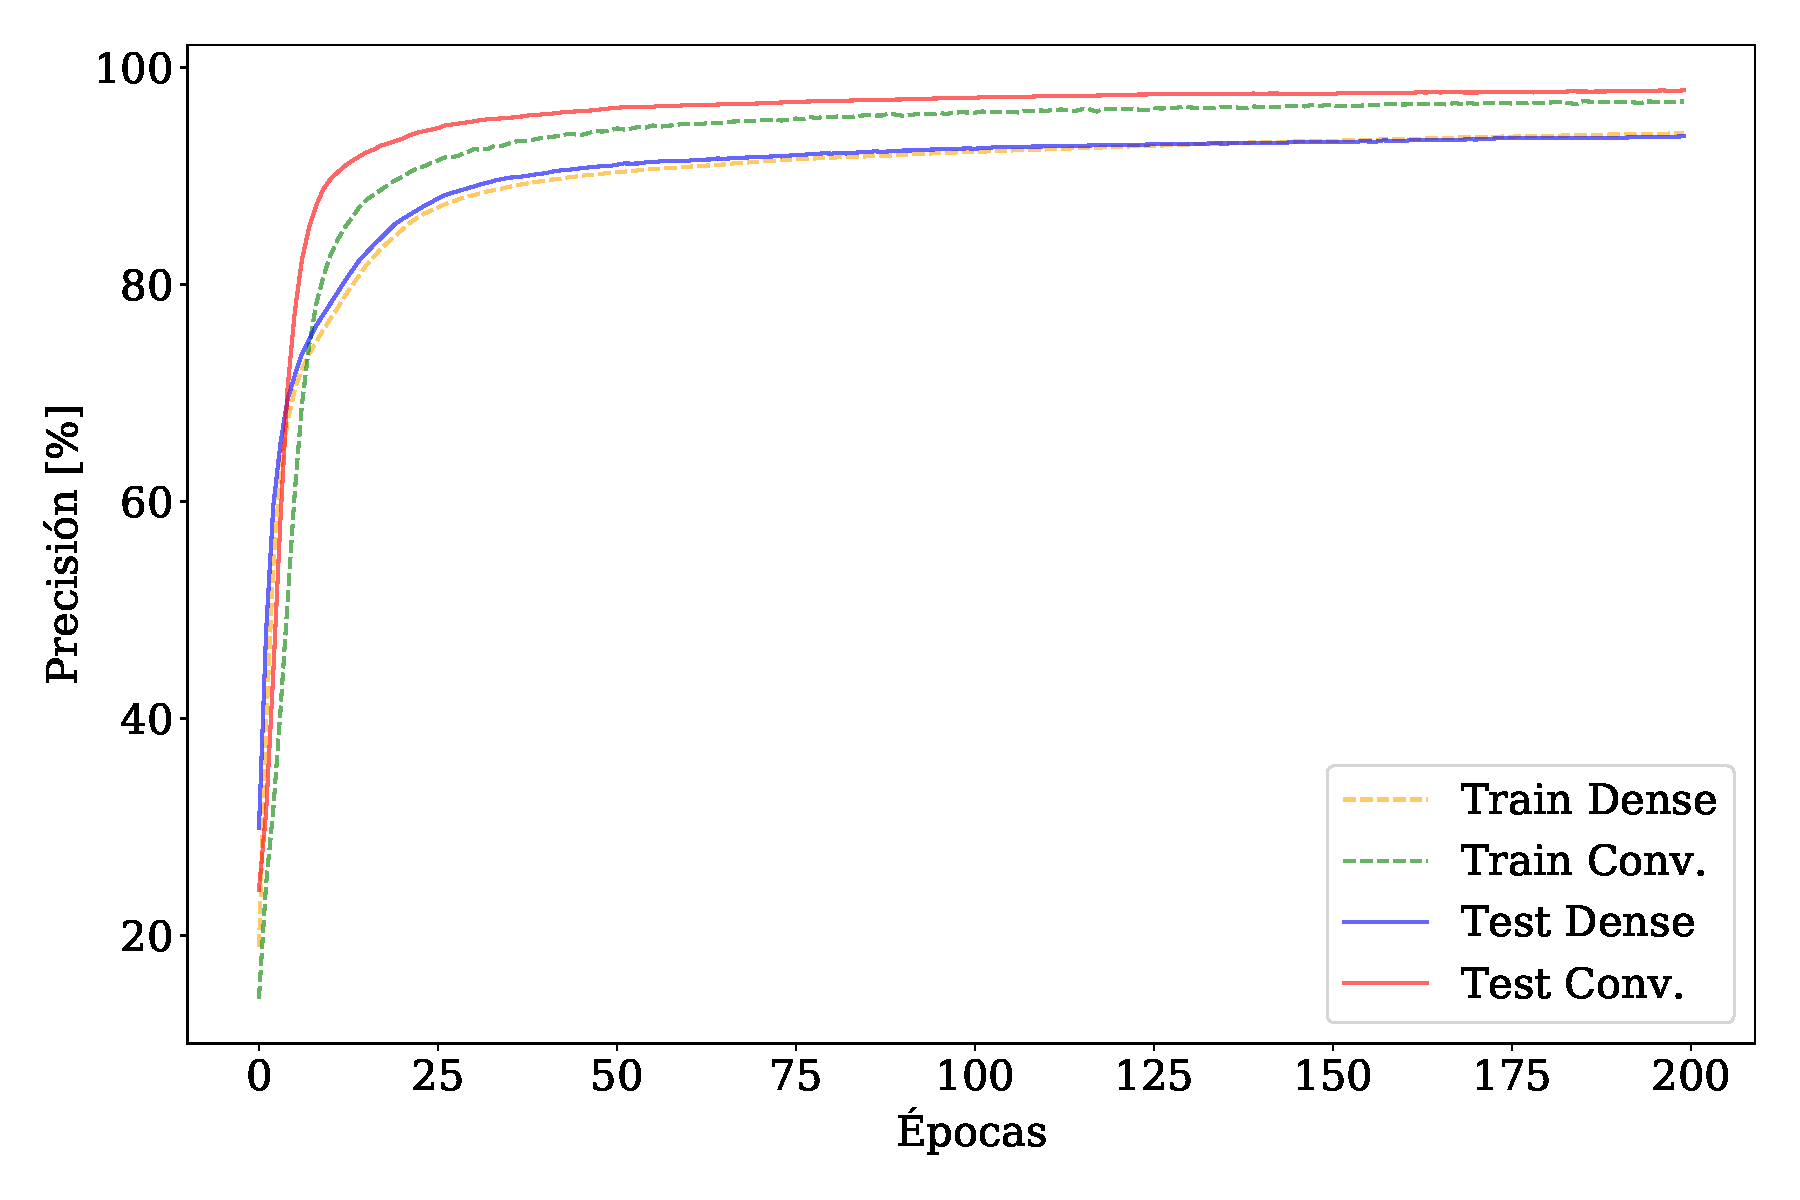
\includegraphics[width=0.47\textwidth]{Graphs/ejer8_acc.pdf}
            \end{center}
            \caption{Precisión de la red en función de las épocas}
            \label{fig:ejer8_acc}
        \end{small}
    \end{figure}

    Otro aspecto interesante de la red convolucionales es que también tienen en cuenta  la correlación espacial de los puntos en la imagen. En el caso de la red densa, donde perdemos información sobre los píxeles vecinos al hacer que las imágenes sean unidimensionales. Tenemos información en una dirección pero no podemos sacar información de las curvas que puede tener un dígito por ejemplo.



    \begin{figure}[H]
        \begin{small}
            \begin{center}
                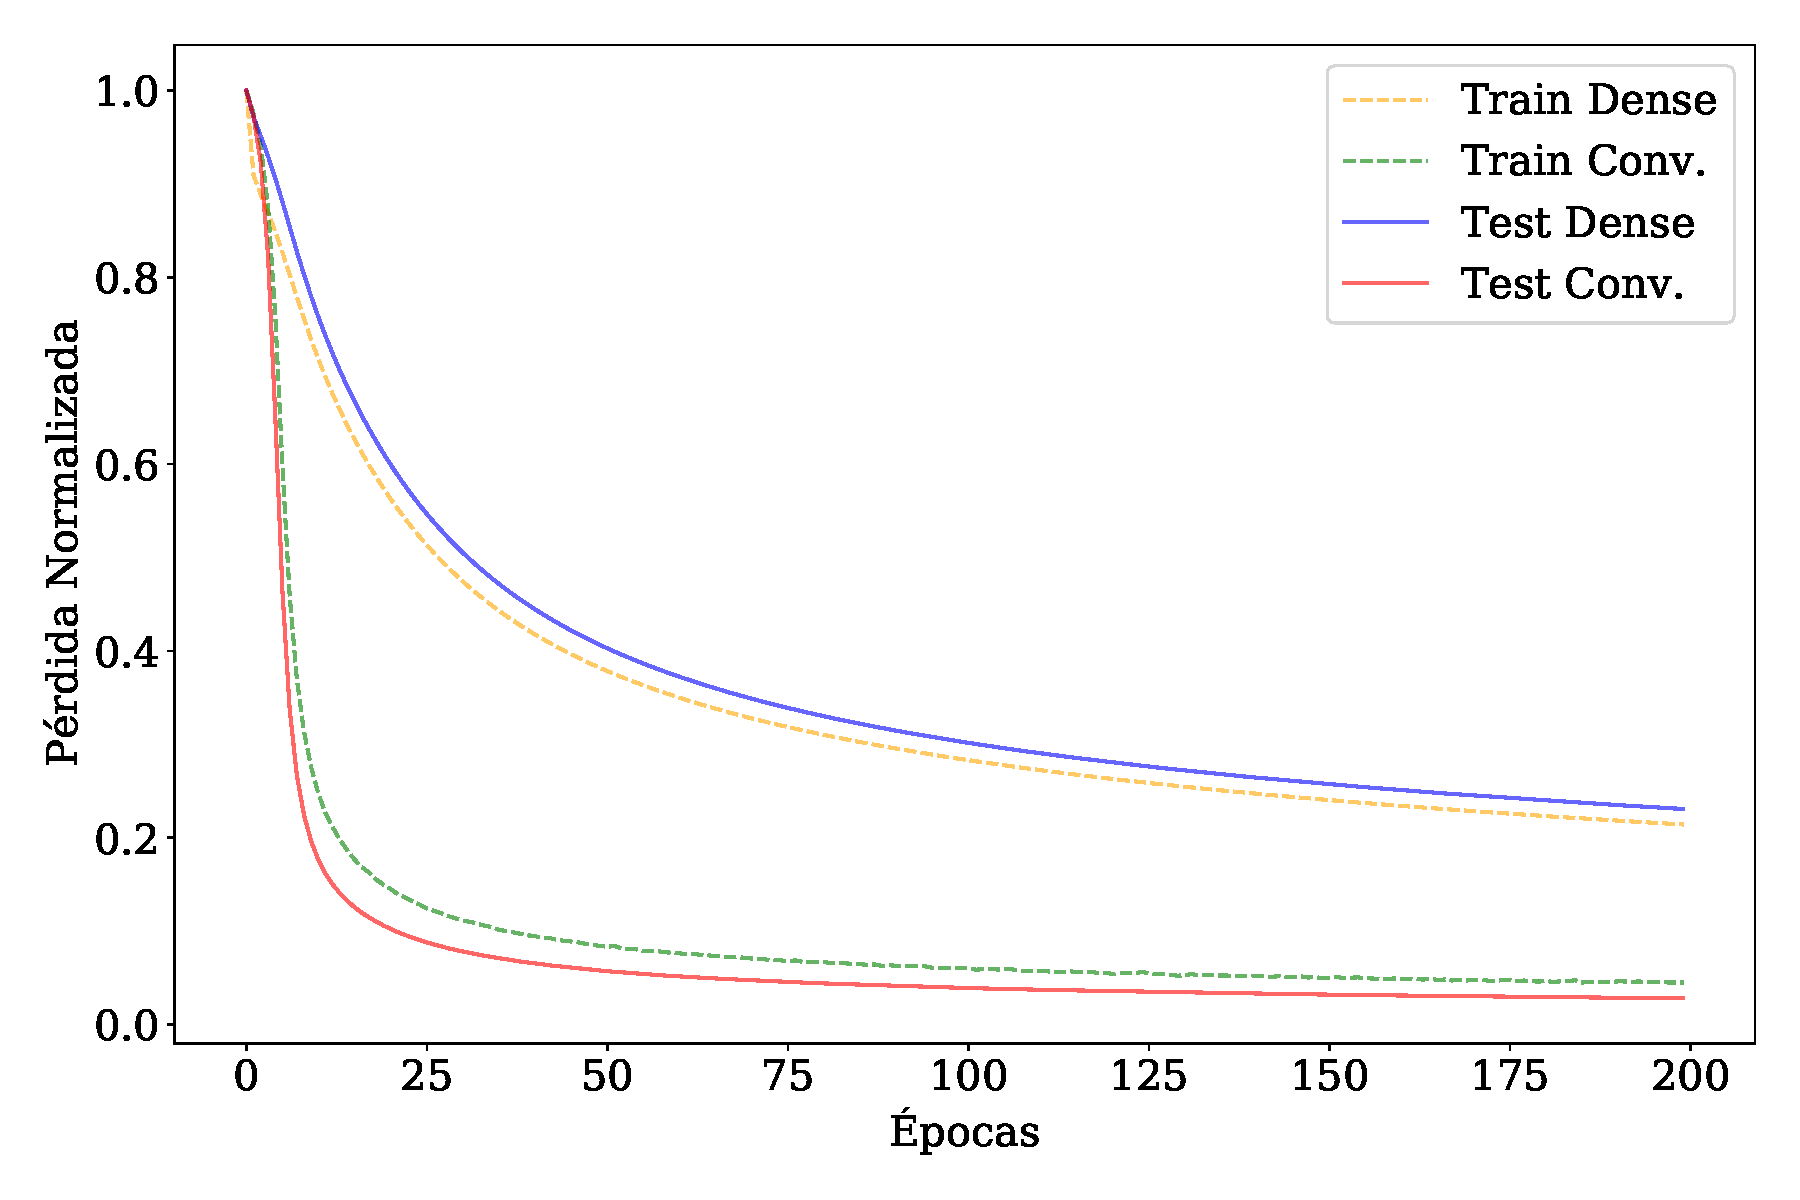
\includegraphics[width=0.5\textwidth]{Graphs/ejer8_loss.pdf}
            \end{center}
            \caption{Pérdida normalizada con respecto al máximo de las redes densa y convolucionales en función de las épocas. }
            \label{fig:ejer8_loss}
        \end{small}
    \end{figure}


\section*{Ejercicio 9}

    Utilizando la red convolucional anterior, volvemos a clasificar las imágenes de los dígitos del MNIST, salvo que ahora hacemos una permutación de los valores de intensidad de los píxeles. 

    En las Figs. \ref{fig:ejer9_acc} y \ref{fig:ejer9_loss} se muestran las curvas de precisión y pérdida normalizada para la red con los datos originales y permutados. La red entrenada los datos permutados alcanza una precisión  de $93.8\%$, que es menor con respecto a la red entrenada con los datos originales. Esto se debe a que se pierde información de la correlación especial de los píxeles de un dígito, como el borde, curva y forma. A pesar de esto, la red puede encontrar correlaciones entres los puntos permutados  y aprender a identificar los dígitos modificados.



\section*{Ejercicio 10}

En este ejercicio se implementan redes similares a las redes AlexNet y VGG16 para clasificar las imágenes de CIFAR-10 y CIFAR-100. Estas redes convolucionales se estructuraron como se muestra a continuación:

    \begin{figure}[H]
        \begin{small}
            \begin{center}
                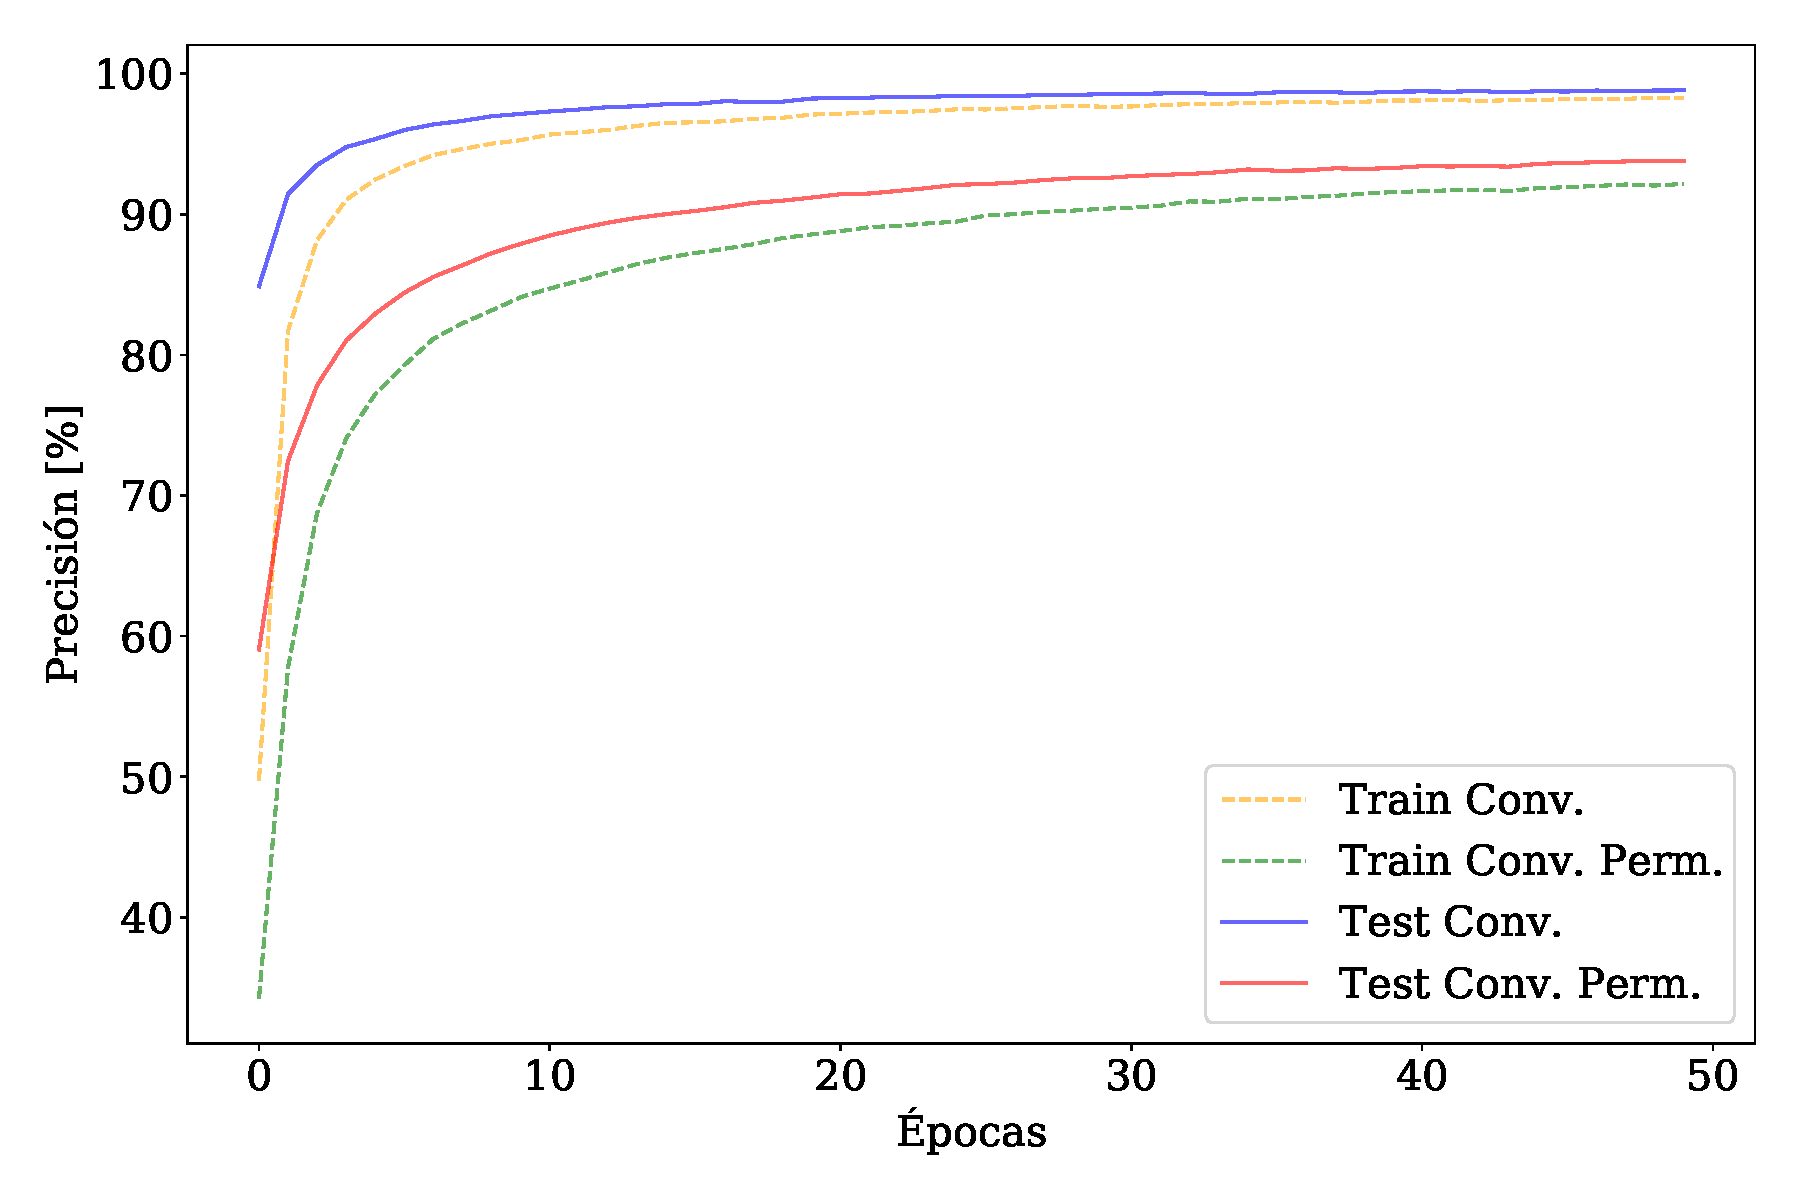
\includegraphics[width=0.5\textwidth]{Graphs/ejer9_acc.pdf}
            \end{center}
            \caption{Precisión de la red en función de las épocas}
            \label{fig:ejer9_acc}
        \end{small}
    \end{figure}


    \begin{figure}[H]
        \begin{small}
            \begin{center}
                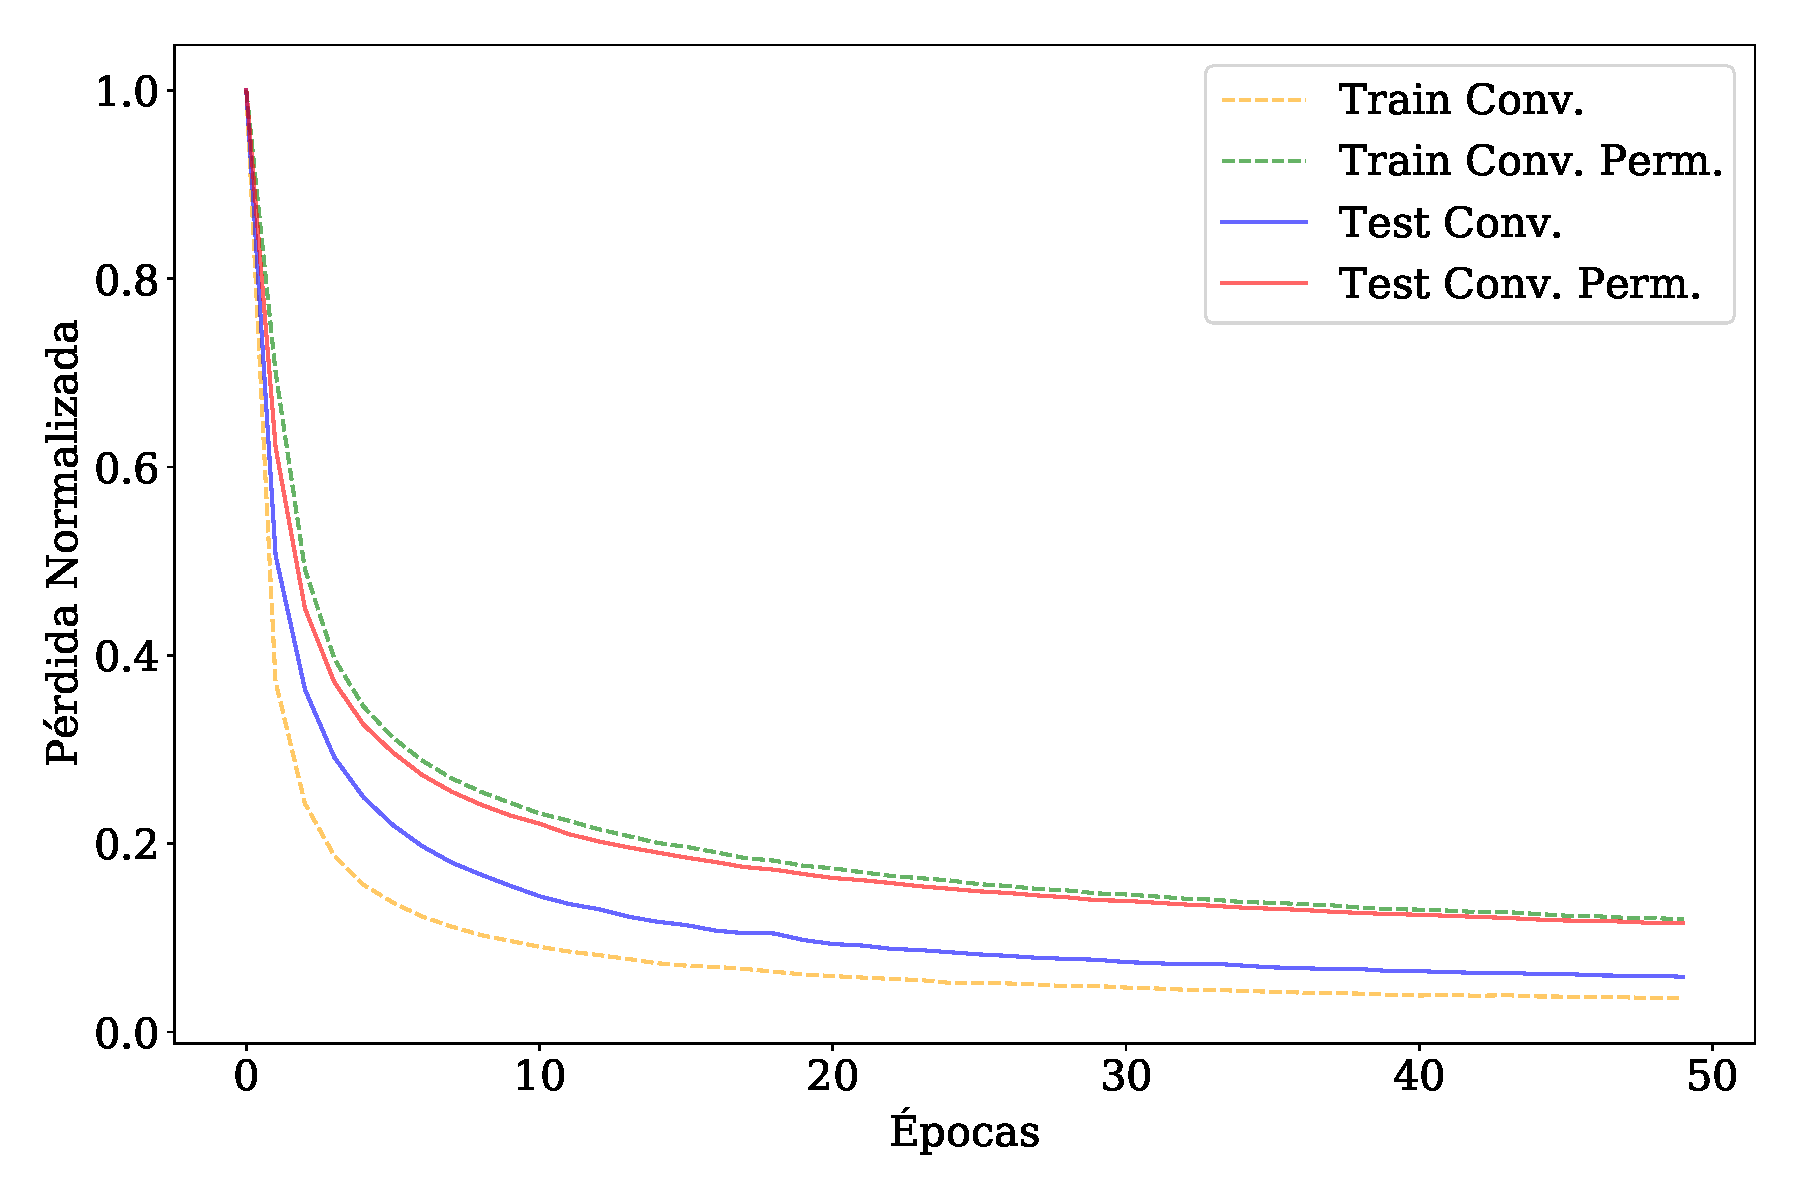
\includegraphics[width=0.5\textwidth]{Graphs/ejer9_loss.pdf}
            \end{center}
            \caption{Pérdida normalizada con respecto al máximo en función de las épocas. }
            \label{fig:ejer9_loss}
        \end{small}
    \end{figure}



\subsection*{Red basada en VGG16}
\begin{verbatim}
Capa                Salida           Parámetros
===============================================
Conv2D              (32, 32, 64)      1792     
_______________________________________________
Conv2D              (32, 32, 64)      36928    
_______________________________________________
MaxPooling2D        (16, 16, 64)      0        
_______________________________________________
Conv2D)             (16, 16, 128)     73856    
_______________________________________________
MaxPooling2D        (8, 8, 128)       0        
_______________________________________________
Conv2D              (8, 8, 256)       295168   
_______________________________________________
Conv2D              (8, 8, 256)       590080   
_______________________________________________
MaxPooling2D        (4, 4, 256)       0        
_______________________________________________
Conv2D              (4, 4, 512)       1180160  
_______________________________________________
MaxPooling2D        (2, 2, 512)       0        
_______________________________________________
Conv2D              (2, 2, 512)       2359808  
_______________________________________________
MaxPooling2D        (1, 1, 512)       0        
_______________________________________________
Flatten             (512)             0        
_______________________________________________
Dense                                          
Activación: ReLU    (1000)            513000   
Regul.: L2(0.001)
_______________________________________________
Dense                                          
Activación: ReLU    (1000)            1001000  
Regul.: L2(0.001)
_______________________________________________
Dense                                          
Activación: Lineal  (100)             100100   
Regul.: L2(0.001)
===============================================
Total parámetros: 6,151,892
\end{verbatim}

\subsection*{Capa basada en AlexNet}

\begin{verbatim}
Capa                Salida           Parámetros
===============================================
Conv2D              (16, 16, 96)     34944  
_______________________________________________
MaxPooling2D        (8, 8, 96)       0      
_______________________________________________
Conv2D              (8, 8, 256)      614656 
_______________________________________________
MaxPooling2D        (4, 4, 256)      0      
_______________________________________________
Conv2D              (4, 4, 256)      590080 
_______________________________________________
Conv2D              (4, 4, 192)      442560 
_______________________________________________
MaxPooling2D        (2, 2, 192)      0      
_______________________________________________
Flatten             (768)            0      
_______________________________________________
Batch Normalization (768)            3072   
_______________________________________________
Dense                                          
Activación: ReLU    (2048)           1574912
_______________________________________________
Dense                                          
Activación: ReLU    (500)            1024500
_______________________________________________
Dropout (0.4)       (500)            0      
_______________________________________________
Dense                                          
Activación: Lineal  (100)            50100  
===============================================
Total parámetros: 4,334,824
Parámetros fijos: 1,536
\end{verbatim}


Para estas redes se utilizó el optimizador Adam con una tasa de aprendizaje de 0.001, la función CCE como función de pérdida y la función \verb|CategoricalAccuracy| como métrica.

Las curvas obtenidas con estas redes se muestran en las Figs. \ref{fig:ejer10_acc_cifar10} y \ref{fig:ejer10_loss_cifar10}. En este trabajo, la red basada en la red VGG 16 obtuvo la mejor precisión en clasificar el CIFAR-10

\begin{figure}[H]
    \begin{small}
        \begin{center}
            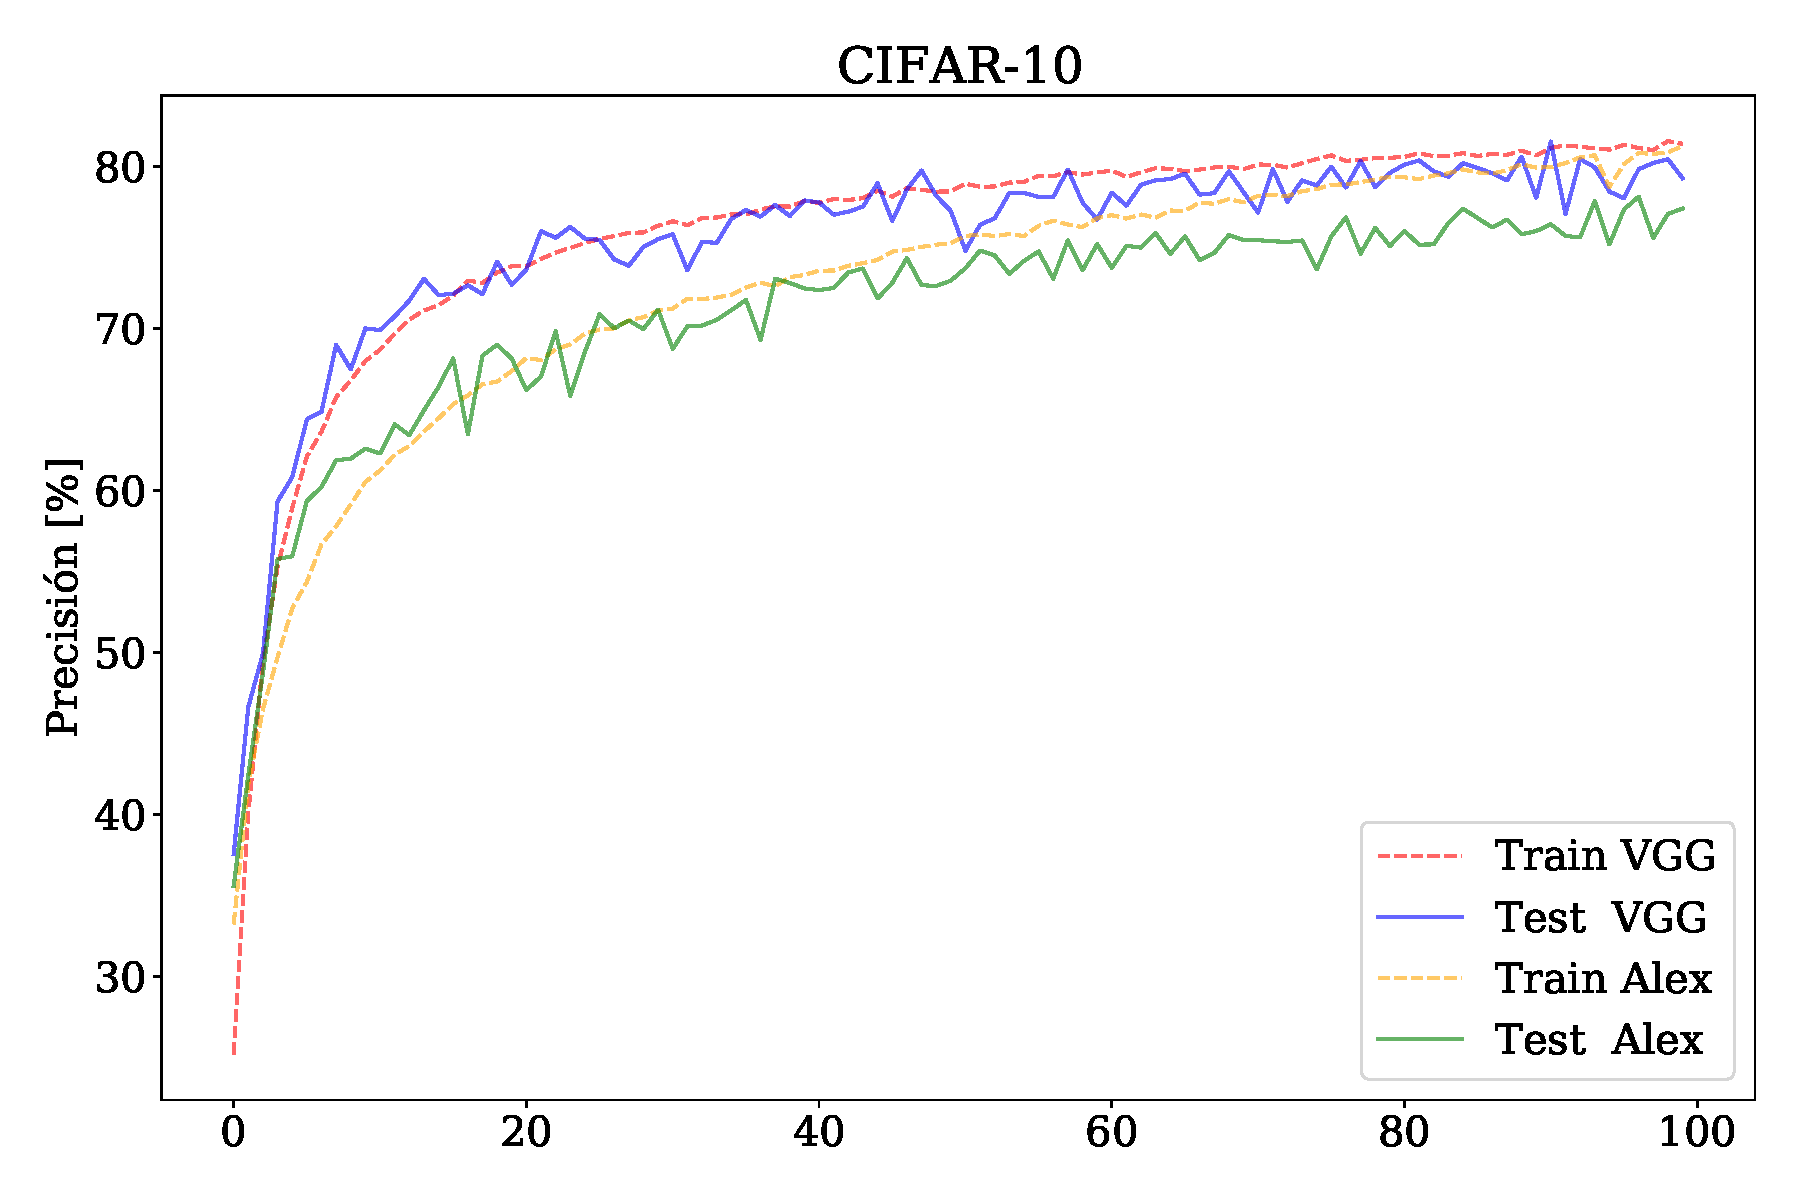
\includegraphics[width=0.45\textwidth]{Graphs/ejer10_acc_cifar10.pdf}
        \end{center}
        \caption{Precisión para el CIFAR-10 con distintas redes en función de las épocas}
        \label{fig:ejer10_acc_cifar10}
    \end{small}
\end{figure}


\begin{figure}[H]
    \begin{small}
        \begin{center}
            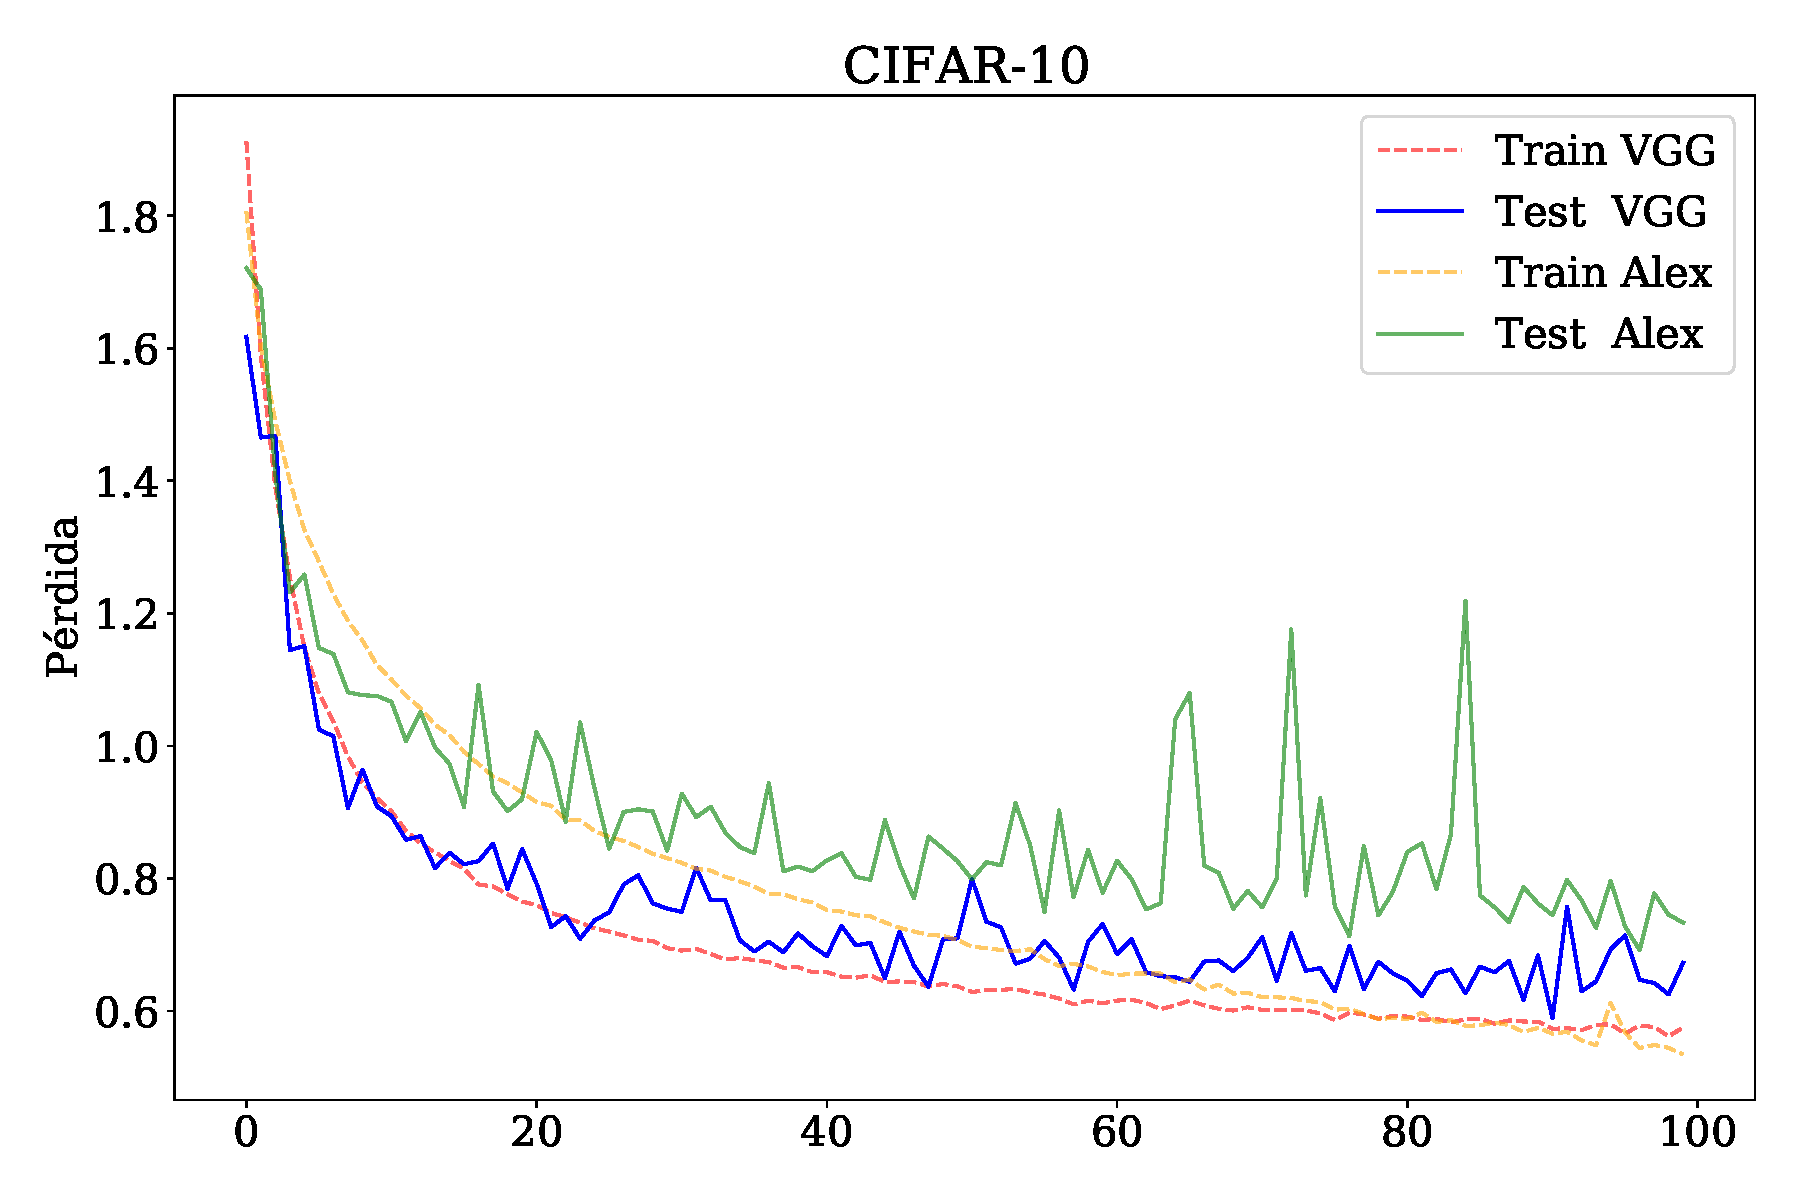
\includegraphics[width=0.45\textwidth]{Graphs/ejer10_loss_cifar10.pdf}
        \end{center}
        \caption{Pérdida para el CIFAR-10 con distintas redes en función de las épocas}
        \label{fig:ejer10_loss_cifar10}
    \end{small}
\end{figure}

Las Figs. \ref{fig:ejer10_acc_cifar100} y \ref{fig:ejer10_loss_cifar100} muestran la precisión y pérdida de las redes implementadas. En este caso También la red basada en la red VGG 16 obtuvo la mejor precisión en clasificar el CIFAR-100, aunque la red presenta un overfitting y es muy ruidosa. En este trabajo no se encontró parámetros que resulten en mejores curvas.


\begin{figure}[H]
    \begin{small}
        \begin{center}
            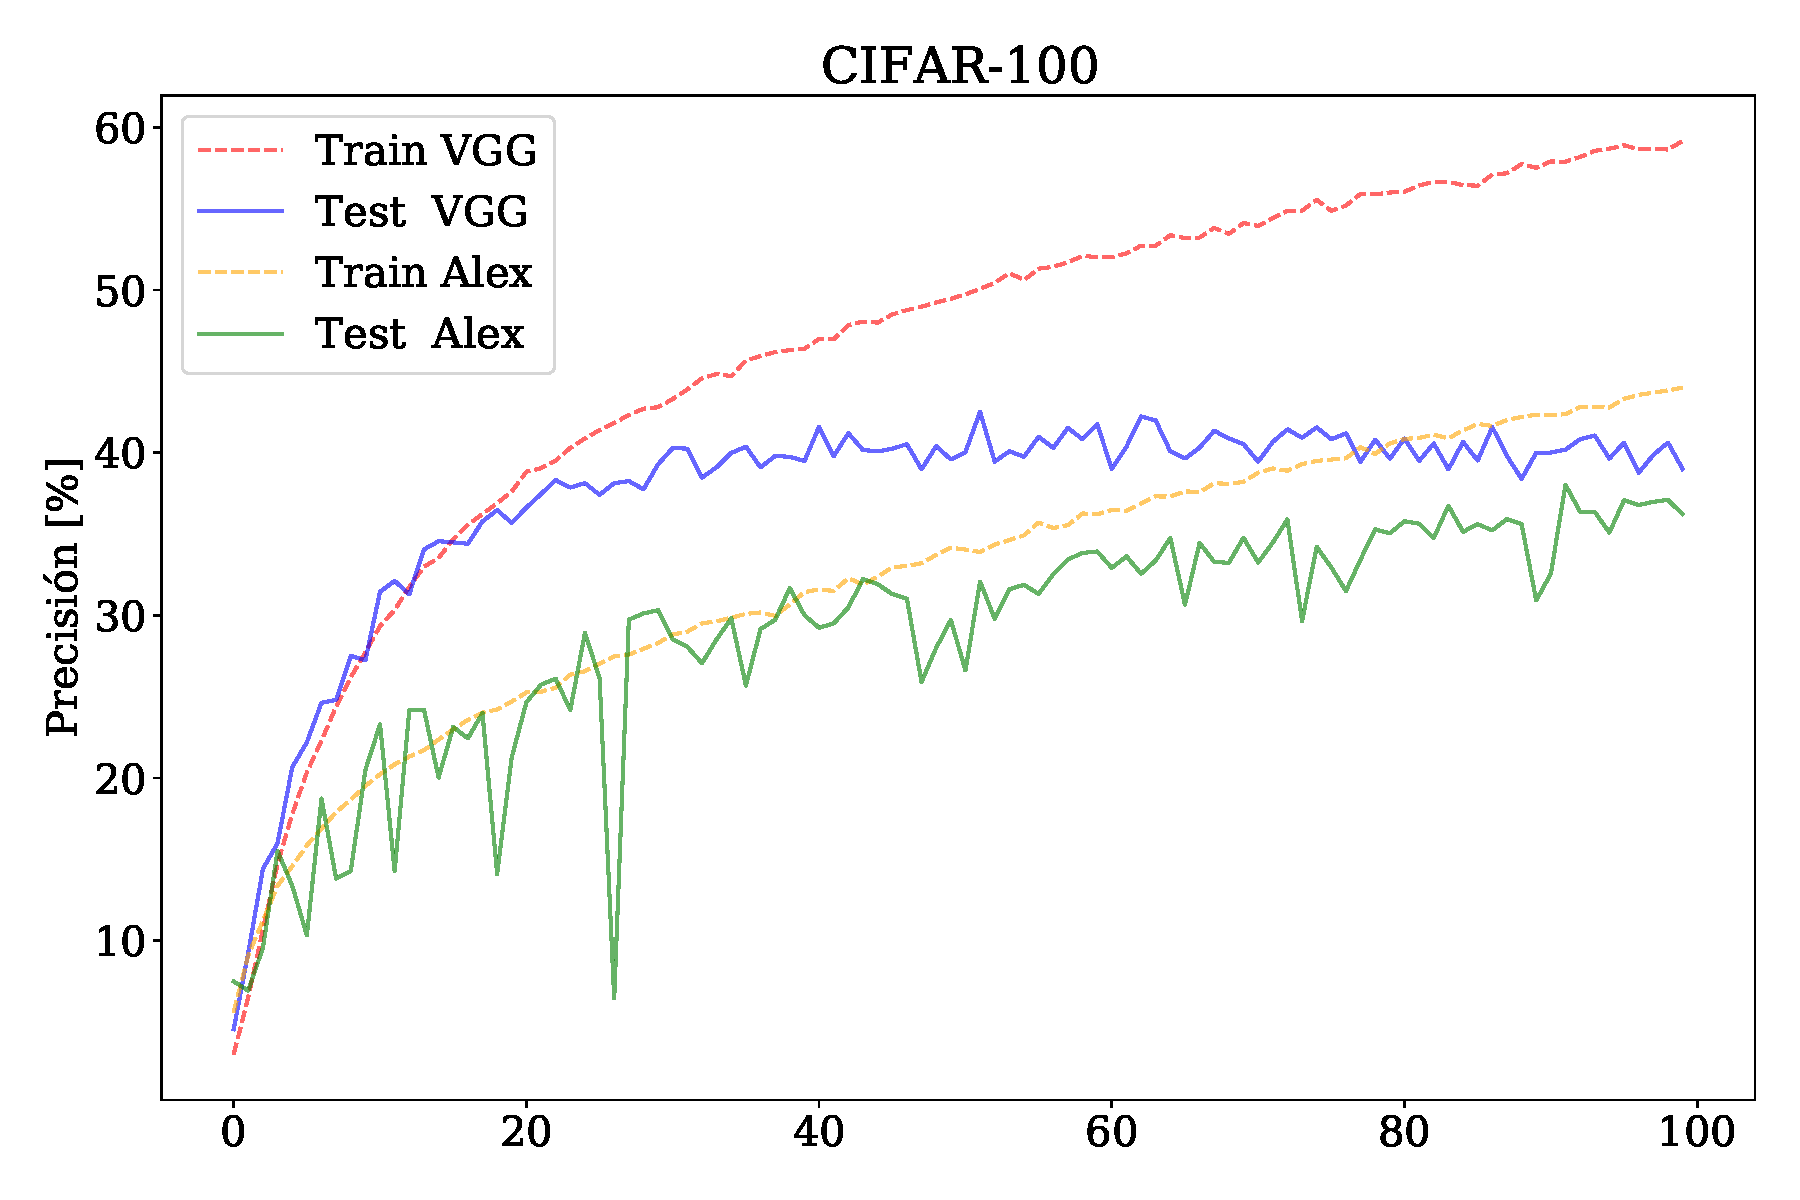
\includegraphics[width=0.5\textwidth]{Graphs/ejer10_acc_cifar100.pdf}
        \end{center}
        \caption{Precisión para el CIFAR-100 con distintas redes en función de las épocas}
        \label{fig:ejer10_acc_cifar100}
    \end{small}
\end{figure}
\vfill\eject
\begin{figure}[H]
    \begin{small}
        \begin{center}
            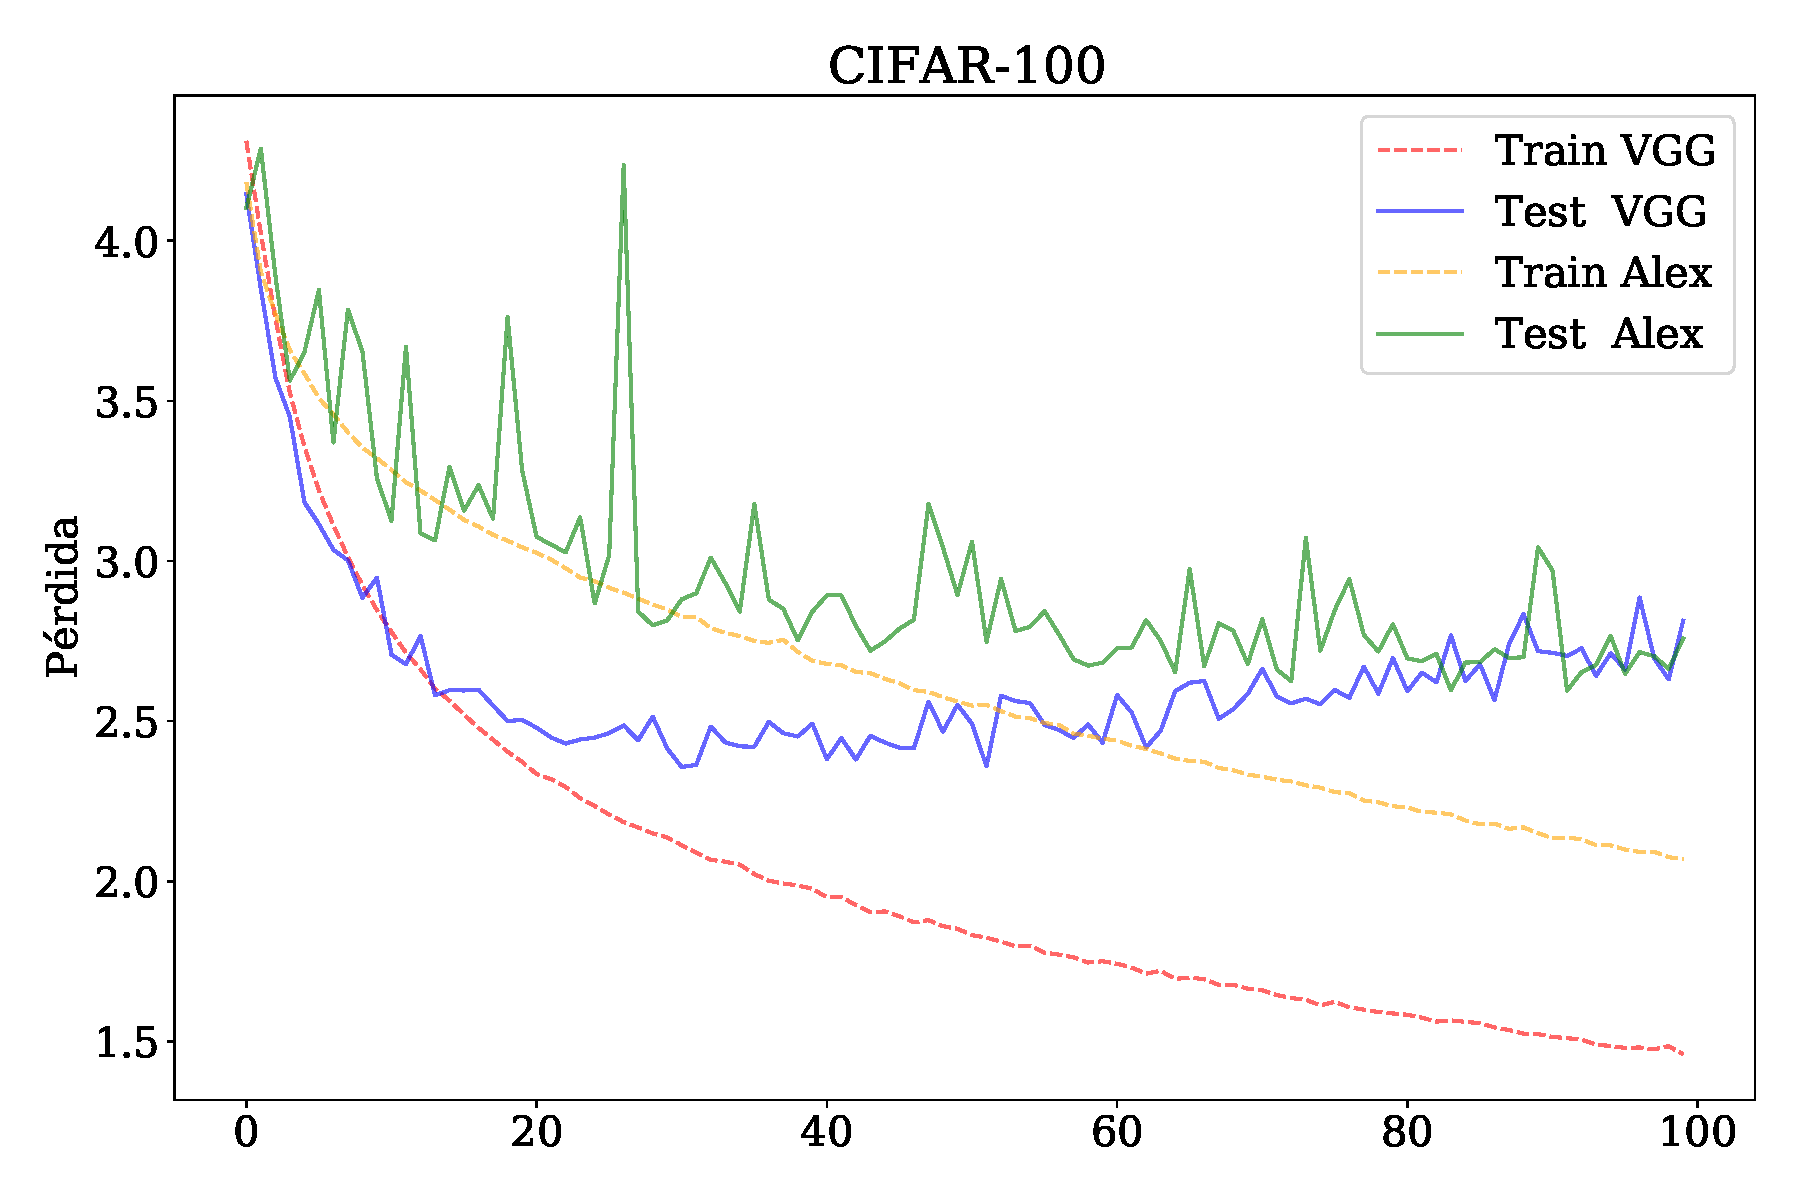
\includegraphics[width=0.5\textwidth]{Graphs/ejer10_loss_cifar100.pdf}
        \end{center}
        \caption{Pérdida para el CIFAR-100 con distintas redes en función de las épocas}
        \label{fig:ejer10_loss_cifar100}
    \end{small}
\end{figure}

\begin{thebibliography}{99}


\bibitem{pima} Smith,J.W., Everhart,J.E., Dickson,W.C., Knowler,W.C., \& Johannes,R.S. (1988). Using the ADAP learning algorithm to forecast
the onset of diabetes mellitus.  In {\it Proceedings of the Symposium on Computer Applications and Medical Care} (pp. 261--265).  IEEE
Computer Society Press.
\end{thebibliography}

\end{document}